%
% PROJECT: <ETD> Electronic Thesis and Dissertation Initiative
%   TITLE: LaTeX report template for ETDs in LaTeX
%  AUTHOR: Neill Kipp, nkipp@vt.edu
%     URL: http://etd.vt.edu/latex/
% SAVE AS: etd.tex
% REVISED: September 6, 1997 [GMc 8/30/10]
% 

% Instructions: Remove the data from this document and replace it with your own,
% keeping the style and formatting information intact.  More instructions
% appear on the Web site listed above.

\documentclass[12pt,english]{report}

\makeatletter
\newif\if@restonecol

\let\algorithm\relax
\let\endalgorithm\relax
%\usepackage[tight,footnotesize]{subfigure}
\usepackage{subfigure}
\usepackage {paralist}
\usepackage{comment}
\usepackage{array}
\usepackage{amsmath}
\usepackage{graphicx}
\usepackage{amssymb}
\usepackage{cite}
\usepackage{url}
\usepackage[ruled]{algorithm2e}
\usepackage{babel}
\makeatother
\makeatletter
\providecommand{\tabularnewline}{\\}


\newtheorem{clm}{Claim}
\newtheorem{proof}{Proof}
\newtheorem{mydef}{Definition}


\makeatletter

%%%%%%%%%%%%%%%%%%%%%%%%%%%%%% LyX specific LaTeX commands.
\pdfpageheight\paperheight
\pdfpagewidth\paperwidth

%% Because html converters don't know tabularnewline
\providecommand{\tabularnewline}{\\}
%% A simple dot to overcome graphicx limitations
\newcommand{\lyxdot}{.}


%%%%%%%%%%%%%%%%%%%%%%%%%%%%%% User specified LaTeX commands.



\makeatother



\setlength{\textwidth}{6.5in}
\setlength{\textheight}{8.5in}
\setlength{\evensidemargin}{0in}
\setlength{\oddsidemargin}{0in}
\setlength{\topmargin}{0in}

\setlength{\parindent}{0pt}
\setlength{\parskip}{0.1in}

% Uncomment for double-spaced document.
% \renewcommand{\baselinestretch}{2}

% \usepackage{epsf}

\begin{document}

\thispagestyle{empty}
\pagenumbering{roman}
\begin{center}

% TITLE
{\Large 
On the Design of Contention Managers for Real-Time Software Transactional Memory
}

\vfill

Mohammed Elshambakey

\vfill

Preliminary Examination Proposal submitted to the Faculty of the \\
Virginia Polytechnic Institute and State University \\
in partial fulfilment of the requirements for the degree of

\vfill

Doctor of Philosophy \\
in \\
Computer Engineering

\vfill

Binoy Ravindran, Chair \\
Robert P. Broadwater \\
Cameron D. Patterson \\
Mohamed Rizk Mohamed. Rizk\\
Anil Kumar S. Vullikanti

\vfill

\textbf{TO BE SPECIFIED}\\
Blacksburg, Virginia

\vfill

Keywords: Software Transactional Memory, Embedded Systems, Contention Managers
\\
Copyright \textbf{TO BE SPECIFIED}, Mohammed Elshambakey

\end{center}

\pagebreak

\thispagestyle{empty}
\begin{center}

{\large On the Design of Contention Managers for Real-Time Software Transactional Memory}

\vfill

Mohammed Elshambakey

\vfill

(ABSTRACT)

\vfill

\end{center}

Real-time systems is concerned with time constraints imposed on a set of tasks executed on one or more processors. Each task consists of a set of instances (jobs). Each job can be repeated exactly at fixed time interval (periodic), or at least at fixed time interval (sporadic). Each job has an absolute deadline. Hard real-time systems (HRT) do not allow jobs to exceed their absolute deadline, while soft real-time systems (SRT) permit exceeding absolute deadlines within upper bound. Real-time schedulers try to satisfy deadline constraints for HRT, and bounding tardiness (the amount of time that a job exceeds its absolute deadline) for SRT. Global Earliest Deadline First (G-EDF) and Global Rate Monotonic Assignment (G-RMA) are two examples of multiprocessor real-time schedulers. G-EDF gives a higher priority to the instance of earliest absolute deadline, while G-RMA gives higher priority to instance of smallest period.

Tasks may need to access common objects through read/write operations. Different instances can conflict if they try to access the same object, and at least one instance is writing to it. Thus, in addition to real-time scheduling, concurrency control is needed for real-time systems. Concurrency control for real-time system should consider time constraints. A number of real-time concurrency control methods were introduced based on locking, lock-free and wait-free algorithms. Lock-based concurrency control suffers from programmability, scalability, and compositionality challenges. These challenges are exacerbated in emerging multicore architectures, on which improved software performance must be achieved by exposing greater concurrency. Lock-free and wait-free offer numerous advantages over locks (e.g., deadlock-freedom), but their programmability has remained a challenge. Past studies show that they are best suited for simple data structures where their retry cost is competitive to the cost of lock-based synchronization.

Transactional memory (TM) is an alternative synchronization model for shared in-memory data objects that promises to alleviate difficulties in locking and lock-free algorithms.  With TM, programmers write concurrent code using threads, but organize code that read/write shared objects as transactions, which appear to execute atomically. Two transactions conflict if they access the same object and one access is a write. When that happens, a contention manager (or CM) resolves the conflict by aborting one and allowing the other to proceed to commit, yielding (the illusion of) atomicity. Aborted transactions are re-started, often immediately. The time consumed by a transaction in abortion and retrying is known as retry cost. In addition to a simple programming model, TM provides performance comparable to highly concurrent fine-grained locking and lock-free approaches, and is composable. TM is semantically simpler and is often the only viable lock-free solution for complex data structures and nested critical sections. Multiprocessor TM has been proposed in hardware, called HTM, and in software, called STM, with the usual tradeoffs: HTM provides strong atomicity, has lesser overhead, but needs transactional support in hardware; STM is available on any hardware. 

In this dissertation proposal, we consider STM for concurrency control in multicore real-time software. Doing so will require bounding transactional  retries, as real-time threads, which subsume transactions, must satisfy time constraints.  Retry bounds in STM are dependent on the CM policy at hand (analogous to the way thread response time bounds are scheduler-dependent). Thus, real-time CM is logical.

We investigate and design a number of real-time CMs. The first two CMs are directly based on dynamic and static priority of underlying tasks. Earliest Deadline-First CM with G-EDF scheduler (ECM) resolves conflicts based on absolute deadline of the underlying instances. Rate Monotonic Assignment with G-RMA scheduler (RCM) resolves conflicts based on period of underlying instances. We analyze retry cost and response time under ECM and RCM. We analytically and experimentally compare their schedulability against lock-free method.

ECM and RCM conserve the semantics of the underlying real-time scheduler. This conservative approach results in a maximum retry cost- for a single transaction due to another transaction- of double the maximum atomic section length among all tasks. So, another CM is developed to reduce this retry cost. Length-based CM (LCM) considers not only static/dynamic priority of underlying instance, but also length of the interfering transaction compared to remaining length of interfered transaction. LCM is used with G-EDF and G-RMA. Although it can reduce retry cost, but it suffers from priority inversion. By proper choice of different parameters, additional cost due to priority inversion can be kept lower than reduced retry cost. Thus, the net result will be lower response time for tasks using LCM with G-EDF/G-RMA. We analyze retry cost and response time of LCM. We analytically and experimentally compare LCM schedulability against ECM, RCM and lock-free.

ECM, RCM and LCM are affected by transitive retry. Transitive retry enforces a transaction to abort and retry due to another non-conflicting transaction. Transitive retry appears when multiple objects exist per transaction. So, we develop the Priority-based with Negative value and First access (PNF) contention manager. PNF avoids transitive retry and deals better with multiple objects than previous contention managers. PNF also tries to optimize processor usage by lowering priority of the job underlying retrying transaction. Thus, other jobs can proceed if there is no conflict. We upper bound retry cost and response time for PNF when used with G-EDF and G-RMA. Schedulability is compared between PNF on one side and ECM, RCM, LCM and lock-free on the other. We experimentally compare retry cost of PNF compared to other synchronization techniques.


\vfill

% GRANT INFORMATION

%\textbf{NEEDS TO BE WRITTEN}

\pagebreak

% Dedication and Acknowledgments are both optional
% \chapter*{Dedication}
% \chapter*{Acknowledgments}

\tableofcontents
\pagebreak

\listoffigures
\pagebreak

\listoftables
\pagebreak

\listofalgorithms
\pagebreak

\pagenumbering{arabic}
\pagestyle{myheadings}

\chapter{Introduction}
\markright{Mohammed Elshambakey \hfill Chapter 1. Introduction \hfill}

Data structure implementation affects degree of exploited parallilsm
in the system \cite{shavit2011data}. As the implementation moves
from lock-based to non-blocking, more parallilism can be exploited.
Thus, more computation speed-up, but more complex design. Things become
more complicated when it comes to synchronization under real-time
multiprocessor systems. Real-time systems should meet deadline of
each task as much as possible. With shared objects, tasks have to
execute in a serial order to some degree when accessing shared objects.
The major problem arises when one of the accesses is a \textit{write}
operation. Conflict resultion techniques is used to decide how to
access these shared objects. In lock-based systems, tasks try to obtain
an object's lock before accessing it. While in lock-free techniques,
some intuition is used to allow tasks to simultaneously access the
object without violating consistency. Different synchronization techniqes
affect response time of each task. Depending on the rationale of conflict
resolution, a task might have to wait for all other interfering tasks
before it can access the required object.

\subsection{Preliminaries}
We consider a multiprocessor system with $m$ identical processors and $n$ sporadic tasks $\tau_1, \tau_2,\ldots, \tau_n$. The $k^{th}$ instance (or job) of a task $\tau_i$ is denoted $\tau_i^k$. Each task $\tau_i$ is specified by its worst case execution time (WCET) $c_i$, its minimum period $T_i$ between any two consecutive instances, and its relative deadline $D_i$, where $D_i=T_i$. Job $\tau_i^j$ is released at time $r_i^j$ and must finish no later than its absolute deadline $d_i^j=r_i^j+D_i$. Under a fixed priority scheduler such as G-RMA, $p_i$ determines $\tau_i$'s (fixed) priority and it is constant for all instances of $\tau_i$. Under a dynamic priority scheduler such as G-EDF, $\tau_i^j$'s priority, $p_i^j$, is determined by its absolute deadline. 
A task $\tau_j$ may interfere with task $\tau_i$ for a number of times during a duration $L$, and this number is denoted as $G_{ij}(L)$. 
$\tau_j$'s workload that interferes with $\tau_i$ during $L$ is denoted $W_{ij}(L)$.

\textit{Shared objects.} A task may need to access (i.e., read, write) shared, in-memory objects while it is executing any of its atomic sections, which are synchronized using STM. 
The set of atomic sections of task $\tau_i$ is denoted $s_i$. $s_i^k$ is the $k^{th}$ atomic section of $\tau_i$. 
Each object, $\theta$, can be accessed by multiple tasks. The set of distinct objects accessed by $\tau_i$ is $\theta_i$. The set of atomic sections used by $\tau_i$ to access $\theta$ is $s_i(\theta)$, and the sum of the lengths of those atomic sections is $len(s_i(\theta))$. $s_i^k(\theta)$ is the $k^{th}$ atomic section of $\tau_i$ that accesses $\theta$. $s_i^k(\theta)$  executes for a duration $len(s_i^k(\theta))$.

If $\theta$ is shared by multiple tasks, then $s(\theta)$ is the set of atomic sections of all tasks accessing $\theta$, and the set of tasks sharing $\theta$ with $\tau_i$ is denoted $\gamma_i(\theta)$. Atomic sections are non-nested. Each atomic section is assumed to access only one object; this allows a head-to-head comparison with lock-free synchronization~\cite{key-5}.  (Allowing multiple object access per transaction is future work.) The maximum-length atomic section in $\tau_i$ that accesses $\theta$ is denoted $s_{i_{max}} (\theta)$, while the maximum one among all tasks is $s_{max} (\theta)$, and the maximum one among tasks with priorities lower than that of $\tau_i$ is $s_{max}^i (\theta)$.

\textit{STM retry cost.} If two or more atomic sections conflict, the CM will commit one section and abort and retry the others, increasing the time to execute the aborted sections. The increased time that an atomic section $s_i^p (\theta)$ will take to execute due to interference with another section $s_j^k (\theta)$, is denoted $W_{i}^{p}(s_{j}^{k}(\theta))$. The total time that a task $\tau_i$'s atomic sections have to retry is denoted $RC(\tau_i)$.
When this retry cost is calculated over the task period $T_i$ or an interval $L$, it is denoted, respectively, as $RC(T_i)$ and $RC(L)$.


\subsection{Summary of Current Research and Contributions}
Contribution of the proposal can be summarized as follows:-
\begin{itemize}
\item We investigate and design priority-based contention managers for real-time systems. These contention managers try to preserve time constraints in addition to data accuracy. For this goal, we investigate Earliest Deadline First contention manager (ECM) and present Rate Monotonic Assignment contention manager (RCM). ECM and RCM keeps the logic of the underlying real-time scheduler (i.e., transaction belonging to higher priority job is allowed to commit first).
\item We present Length-based contention manager (LCM) which can be used with both G-EDF and G-RMA. LCM is not only concerned with priority of the transactions, but also with the length of the interfering transaction relative to the length of the interfered transaction. LCM achieves better retry cost and response time than ECM and RCM.
\item Priority-based with Negative value and First access (PNF) contention manager is introduced. PNF avoids transitive retry effect suffered by ECM, RCM and LCM in case of multiple objects per transaction. PNF tries to optimize processor usage by lower priority of aborted transaction. This way, other tasks can proceed if they do no conflict with others.
\item For previous contention managers, we upper bounded their retry cost and response times. We compared their schedulability to identify the conditions to prefer one of the them over the others. We also compared their schedulability against schedulability of lock-free method. We also compared retry cost of previous synchronization techniques.
\end{itemize}

\subsection{Summary of Proposed Post Preliminary-Exam Work}

Based on our current research results, we proposed the following work:
\begin{itemize}

\item \textbf{Analytical and experimental comparison between developed CMs and real-time locking protocols}
It has been said that lock-free and wait-free methods offer numerous advantages over locking protocols, but locking protocols are still of wide use in real-time systems due to simpler programming and analysis than lock-free. Thus, it is desired to compares different CMs against real-time locking protocols. Examples of real-time locking protocols include PCP and its variants~\cite{chen1990dynamic,6031129,Rajkumar:1991:SRS:532621,sha1990priority}, multiprocessor PCP (MPCP)~\cite{lakshmanan2009coordinated,rajkumar2002real,chen1998multiprocessor,easwaran2009resource}, SRP~\cite{lopez2004utilization}, multiprocessor SRP (MSRP)~\cite{gai2003comparison}, PIP~\cite{easwaran2009resource}, FMLP~\cite{key-4,brandenburg2008implementation,holman2006locking} and OMLP~\cite{Baruah:2007:TMG:1338441.1338647}. OMLP and FMLP are similar, and FMLP was found to be superior to other protocols~\cite{brandenburg2008comparison}.

\item \textbf{Contention manager development for nested transactions}
Transactions can be nested \textit{linearly}, where each transaction has at most one pending transaction~\cite{Moss2006186}. Nesting can also be done in \textit{parallel} where transactions execute concurrently within the same parent~\cite{volos2009nepaltm}. Linear nesting can be \textit{1) flat:} If a child transaction aborts, then parent also aborts. If a child commits, no effect is taken until the parent commits. Modifications made by child transaction is seen only be the parent . \textit{2) Closed:} Similar to \textit{flat nesting} except that if a child transaction aborts, parent does not have to abort. \textit{3) Open:} If a child transaction commits, its modifications is seen not only by the parent, but also by other non-surrounding transactions. If parent aborts after child commits, child modifications are still valid. It is required to extend the proposed real-time CMs (or develop new ones) to handle some or all types of transaction nesting.

\item \textbf{Combine both LCM and PNF} LCM is designed to reduce the retry cost of one transaction when it is interfered close to its end of execution. PNF is designed to avoid transitive retry in case of multiple objects per transactions. One goal is to combine benefits of both algorithms.

\item \textbf{Investigate other criterion for contention managers to further reduced retry cost} Criterion other than or combined with priority, transaction length and first access may be used to produce better contention managers.

\end{itemize}

\subsection{Proposal outline}
The rest of this dissertation proposal is organized as follows. Chapter~\ref{related_work} overviews past and related work for real-time concurrency control. Chapter~\ref{ecm-rcm} investigates Earliest Deadline First CM (ECN) and proposes Rate-Monotnic Assignment CM (RCM). We derive upper bounds for retry cost and response time under ECM and RCM. Finally, schedulability is compared between ECM, RCM and lock-free method. Chapter~\ref{ch_lcm} shows how to reduce retry cost of transactions under ECM and RCM using a length-based CM (LCM). Chapter~\ref{ch_pnf} tries to solve transitive retry of transaction under ECM, RCM and LCM in case of multiobjects per transaction. Chapter~\ref{ch_exp} compares measured retry cost and response time for sets of tasks under previous CMs, as well as, lock-free algorithm. We conclude in Chapter~\ref{conclusions}.

%%%%%%%%%%%%%%%%%%%%%%%%%%%%%%%%

\chapter{\label{related_work}Past and Related Work}
\markright{Mohammed Elshambakey \hfill Chapter 2. Past and Related Work \hfill}

\subsection{Real-Time Lock-free Synchronization}

Transactional-like concurrency control and lock-free synchronization,
for real-time systems, has been previously studied in (e.g.,~\cite{anderson95realtime,anderson1997lock,684918,1203552,896371,anderson96framework,811240}).
Despite their numerous advantages over locks (e.g., deadlock-freedom),
their programmability has remained a challenge. Past studies show
that they are best suited for simple data structures where their retry
cost is competitive to the cost of lock-based synchronization~\cite{bc+08,key-5}.
In contrast, STM is semantically simpler~\cite{Herlihy:2006:AMP:1146381.1146382},
and is often the only viable lock-free solution for complex data structures
(e.g., red/black tree) \cite{6045438} and nested critical sections
\cite{Saha:2006:MHP:1122971.1123001,Agrawal:2008:SOT:1378533.1378553,Peri:2011:CCE:1946143.1946152}.


\subsection{Transactional Memory: Overview }

Transactional memory (TM) is motivated by Database transactions~\cite{Gray:1981:TCV:1286831.1286846}.
In TM, each thread executes a set of transactions when accessing shared memory. A TM transaction consists of a sequence
of steps (i.e., reads and/or writes) executed atomically by a thread \cite{tm-book10}. Atomicity
means that the sequence of steps logically occur at a single instant in time; intermediate states are
invisible to other transactions. The difficulty of locks' maintenance and development are the driving motivation for seeking alternate concurrency control methods.
Lock-free and wait-free are two alternatives. Lock-free and wait-free have high performance, but significantly
complex to write and reason about, and therefore, have largely been
limited to a simple data structures - e.g., linked lists,
queues, stacks \cite{1508449,4079519,1656921,Cho:2006:UAP:1141277.1141490}.

The term \textquotedblleft{}transactional memory\textquotedblright{}
was proposed by Herlihy and Moss~\cite{Herlihy:1993:TMA:165123.165164}, where they presented hardware
support for lock-free data structures. TM has been provided in hardware
(HTM) \cite{Herlihy:1993:TMA:165123.165164,Martinez:2002:SSA:605397.605400,Oplinger:2002:ESR:605397.605417,Rajwar:2002:TLE:605397.605399,ham04},
software (STM) \cite{4145102,Dolev:2008:CSC:1400751.1400769,Harris:2003:LSL:949305.949340,Harris:2005:CMT:1065944.1065952,Cho:2006:UAP:1141277.1141490,Marathe:2004:DTM:1066650.1066660,Yoo:2008:ATS:1378533.1378564,Saha:2006:ASS:1194816.1194838,Shpeisman:2007:EIO:1250734.1250744}
and hybrid TM \cite{dam06,Kumar:2006:HTM:1122971.1123003,Minh:2007:EHT:1250662.1250673,Shriraman:2007:IHA:1250662.1250676}.
Hybrid TM allows STM to improve performance using HTM support. Conflicts between TM threads arise when multiple threads try to access the same object simultaneously, and at least one access is a \textit{write} operation. TM uses \textit{Contention Managers} (CM) to resolve these conflicts. CM decides which transaction to abort and when to
restart the aborted transaction in case of conflicts \cite{Spear:2009:CSC:1504176.1504199,Scherer:2005:ACM:1073814.1073861,Blake:2009:PTS:1669112.1669133,Maldonado:2010:SST:1693453.1693465}.

\subsection{Real-Time Database Transactions}

As database transactions motivated TM \cite{Gray:1981:TCV:1286831.1286846}.
Real-time database has a lot of inspiration to real-time transactional
memory \cite{real-time-data-base-systems-book}. Real-time database
is not concerned only with consistency, but also with timing constraints.
When there is a conflict, lower priority transaction is aborted if
it is abortable, or may cause excessive blocking to any higher priority
transaction \cite{liang2003quantification,liang1996bap,lam1997concurrency}.
Blocking time can be estimated by on-line or off-line schedulers.
\cite{liang2003quantification} and \cite{liang1996bap} proposed
a framework for trading abort cost with the blocking cost of transactions.
\cite{xian2009data} and \cite{chen2002efficient} present a number
of transaction scheduling strategies. These strategies include ED
(Earliest Deadline), HV (Highest Value), HRU (Highest Reward and Urgency),
and FHR (Flexible High Reward). \cite{tseng1997adaptive} schedules
transactions on multiprocessor system based on both slack time and
value assigned to each transaction. So, it tries to acheive the highest
possible value of completed transactions and meat as much deadlines
as possible. \cite{yuehua2010new} combines EDF with LSF (Least Slack
First) to compute transaction priorities. Different scheduling strategies compute transactions' priorities, hence, which transaction to commit first.


\subsection{Real-Time STM}

STM concurrency control for real-time systems has been
previously studied in~\cite{manson2006preemptible,fahmy2009bounding,sarni2009real,schoeberl2010rttm,barrosmanaging,6045438,fahmy2009response}.
\cite{manson2006preemptible} proposes a restricted version of STM
for uniprocessors. \cite{fahmy2009response} considers STM for distributed
uni-processor systems. A higher priority task causes only one retry
in a lower prirority tasks due to the uni-prcessor. \cite{fahmy2009bounding}
bounds response times in distributed multiprocessor systems with STM
synchronization. They consider Pfair scheduling, limit to small atomic
regions with fixed size, and limit transaction execution to span at
most two quanta. \cite{sarni2009real} presents real-time scheduling
of transactions and serializes transactions based on transactions'
- not jobs'- deadlines. However, the work does not bound retries and
response times, nor establishes tradeoffs against lock-free synchronization.
\cite{schoeberl2010rttm} proposes real-time HTM. The retry bound
developed in~\cite{schoeberl2010rttm} assumes that the worst case
conflict between atomic sections of different tasks occurs when the
sections are released at the same time. This assmuption deos not cover
the worst case scenario for transactions' interference. \cite{6045438}
presents earliest-deadline CM or ECM. ECM resolves conflicts by aborting
the transaction with longer absoluted deadline. \cite{6045438} derives
a number of properties for ECM, upper bounds transactional retrys,
and compares schedulability of ECM to retry-loop lock-free synchronization
\cite{key-5}. \cite{6045438}, like \cite{schoeberl2010rttm}, assumes
that the worst case conflict between atomic sections occurs when the
sections are released simultaneously. Besides, \cite{6045438} assumes
all transactions have equal lengths. \cite{barrosmanaging} presents
extend idea in \cite{6045438} to bound number of retries and prevent
starvation. \cite{barrosmanaging} presents three ideas for CMs. However,
work in \cite{barrosmanaging} is still in progress. Provided algorithms
might not give the planned results because they are not analyzed.
%%%%%%%%%%%%%%%%%%%%%%%%%%%%%%%%

\chapter{\label{ecm-rcm}ECM and RCM}
\markright{Mohammed Elshambakey \hfill Chapter 3. ECM and RCM \hfill}

We consider software transactional memory (STM) for concurrency control in multicore embedded real-time software. We investigate real-time contention managers (CMs) for resolving transactional conflicts, including those based on dynamic and fixed priorities, and establish upper bounds on transactional retries and task response times. We identify the conditions under which STM (with the proposed CMs) is superior to lock-free synchronization.

\section{G-EDF/EDF CM (ECM)}
\label{sec:g-edf-edf-cm}

Since only one atomic section among many that share the same object can commit at any time under STM, those atomic sections execute in sequential order.  A task $\tau_{i}$'s atomic sections are interfered by other tasks that share the same objects with $\tau_{i}$. Hereafter, we will use \emph{ECM} to refer to a multiprocessor system scheduled by G-EDF and resolves STM conflicts using the EDF CM. ECM was originally introduced in~\cite{6045438}. ECM will abort and retry an atomic section of $\tau_i$, $s_i^k(\theta)$ due to a conflicting atomic section of $\tau_j$, $s_j^l(\theta)$, if the absolute deadline of $\tau_j$ is less than or equal to the absolute deadline of $\tau_i$. ECM behaviour is shown in Algorithm~\ref{ecm_algorithm}. \cite{6045438} assumes the worst case scenario for transactional retry occurs when conflicting transactions are released simultaneously.~\cite{6045438} also assumes all transactions have the same length. Here, we extend the analysis in~\cite{6045438} to a more worse conflicting scenario and consider distinct-length transactions. We also consider lower number of conflicting instances of any job $\tau_j$ to another job $\tau_i$.


\begin{algorithm}
\footnotesize{
\LinesNumbered
\KwData{$s_i^k(\theta)\rightarrow$ interfered atomic section. $s_j^l(\theta)\rightarrow$ interfering atomic section}
\KwResult{which atomic section aborts}
\eIf{$d_i^k < d_j^l$}
	{$s_j^l(\theta)$ aborts\label{step_sicommits}\;}
	{$s_i^k(\theta)$ aborts\label{step_siaborts}\;}
	}
\caption{ECM}
\label{ecm_algorithm}
\end{algorithm}

\subsection{G-EDF Interference and workload}

The maximum number of times a task $\tau_{j}$ interferes with $\tau_{i}$ is given in~\cite{key-2} and is illustrated in Figure~\ref{fig1}. 
Here, the deadline of an instance of $\tau_{j}$ coincides
with that of $\tau_{i}$, and $\tau_{j}^{1}$ is delayed by its maximum
jitter $J_{j}$, which causes all or part of $\tau_{j}^1$'s execution to overlap within $T_i$. From Figure~\ref{fig1}, it is seen that $\tau_{j}$'s maximum workload that interferes with $\tau_{i}$ (when there are no atomic sections) in $T_{i}$ is:
\begin{eqnarray}
W_{ij}\left(T_{i}\right) & \le & \left\lfloor\frac{T_{i}}{T_{j}}\right\rfloor c_{j}+min\left(c_{j},T_{i}-\left\lfloor\frac{T_{i}}{T_{j}}\right\rfloor T_{j}\right)\nonumber \\
 & \le & \left\lceil\frac{T_{i}}{T_{j}}\right\rceil c_{j}\label{eq11}\end{eqnarray}

For an interval $L<T_{i}$, the worst case pattern of interference is shown in Figure~\ref{fig2}. Here, $\tau_{j}^{1}$ contributes by all its $c_j$, and $d_j^{k-1}$ does not have to coincide with $L$, as $\tau_j^{k-1}$ has a higher priority than that of $\tau_{i}$. The workload of $\tau_{j}$ is:
\begin{equation}
W_{ij}\left(L\right)\le \left(\left\lceil\frac{L-c_{j}}{T_{j}}\right\rceil +1\right)c_{j}
\label{eq12}\end{equation}

Thus, the overall workload, over an interval $R$ is:
\begin{equation}
W_{ij}\left(R\right)=min\left(W_{ij}\left(R\right),W_{ij}\left(T_{i}\right)\right)\label{eq13}\end{equation}
where $W_{ij}(R)$ is calculated by~(\ref{eq12}) if $R<T_i$, otherwise, it is calculated by~(\ref{eq11}).

\begin{figure}%[htbp]
\centering
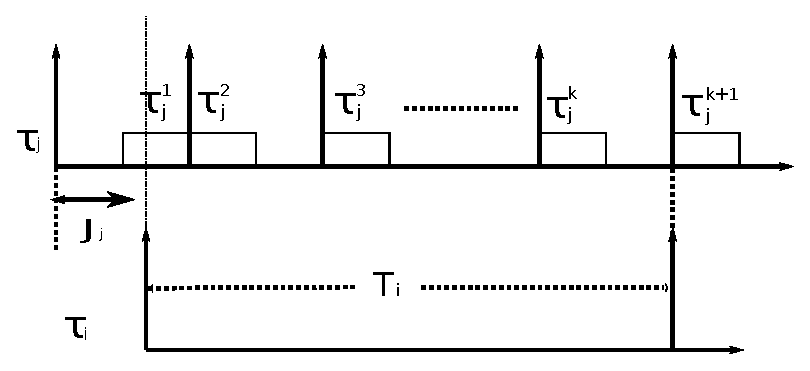
\includegraphics[bb=0bp 0bp 542bp 162bp,scale=0.5]{figures/figure9-a}
\caption{\label{fig1} Maximum interference between two tasks, running on different processors, under G-EDF}
\end{figure}


\begin{figure}
\centering
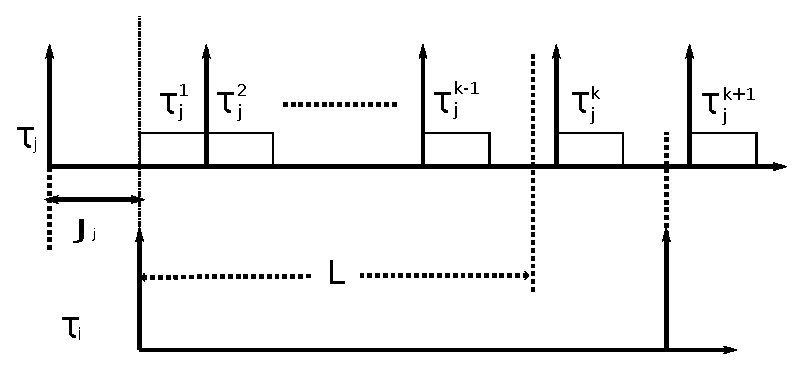
\includegraphics[bb=0bp 0bp 542bp 162bp,scale=0.5]{figures/figure9-b}
\caption{\label{fig2}Maximum interference during an interval $L$ of $T_{i}$}
\end{figure}

\subsection{Retry Cost of Atomic Sections}

\begin{figure*}
\centering
\subfigure[Early validation]{
            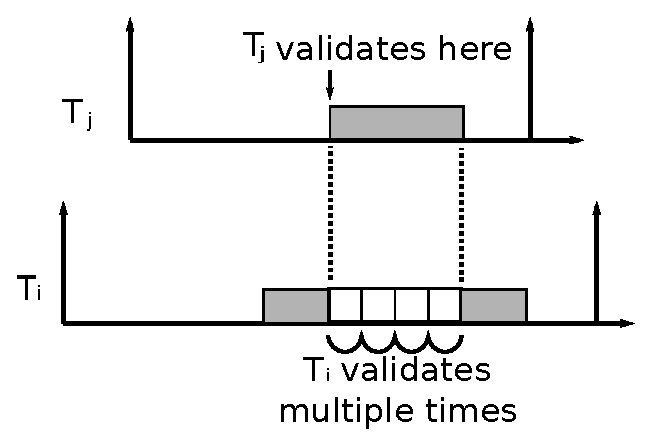
\includegraphics[scale=.45]{figures/figure5-a}
\label{fig5-a} 
}\hspace{1.2cm}
\subfigure[Lazy validation with $len(s_{i}^{k}(\theta))\le len(s_{j}^{l}(\theta))$]{
            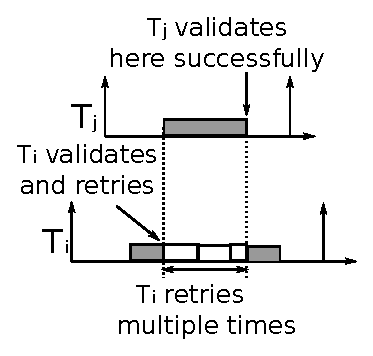
\includegraphics[scale=.65]{figures/figure5-b-1}
\label{fig5-b} 
}\hspace{1.5cm}
\subfigure[Lazy validation with $len(s_{i}^{k}(\theta))>len(s_{j}^{l}(\theta))$]{
            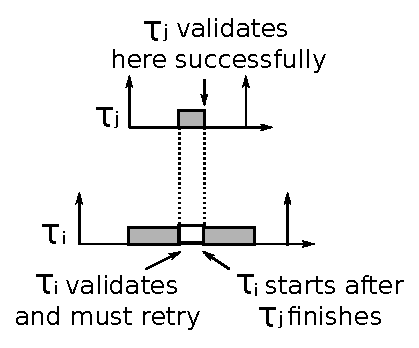
\includegraphics[scale=.65]{figures/figure5-c-1}
\label{fig5-c} 
}
\caption{Retry of $s_i^k(\theta)$ due to $s_j^l(\theta)$}  
\label{fig5}
\end{figure*}


\begin{clm}\label{gedf-edf}
Under ECM, a task $\tau_i$'s maximum retry cost during $T_i$ is upper bounded by:
\begin{eqnarray}
RC\left(T_{i}\right) & \le & \sum_{\theta\in\theta_{i}}\Bigg(\Big(\sum_{\tau_{j}\in\gamma_i(\theta)}\Big(\left\lceil\frac{T_{i}}{T_{j}}\right\rceil\sum_{\forall s_{j}^{l}(\theta)}len\big(s_{j}^{l}(\theta)\nonumber \\
 & + & s_{max}(\theta)\big)\Big)\Big)-s_{max}(\theta)+s_{i_{max}}(\theta)\Bigg)\label{eq3}\end{eqnarray}
\end{clm}
\begin{proof}
Consider two instances $\tau_{i}^a$ and $\tau_{j}^b$, where $d_j^b \le d_i^a$. When a shared object conflict occurs, the EDF CM will commit the atomic section of $\tau_j^b$ while aborting and retrying that of $\tau_i^a$.
Thus, an atomic section of $\tau_i^a$, $s_{i}^{k}(\theta)$,
will experience its maximum delay when it is at the end of its atomic section,  
and the conflicting atomic section of $\tau_j^b$, $s_{j}^{l}(\theta)$, starts, because the whole $s_i^k (\theta)$ will be repeated after $s_j^l (\theta)$.

Validation (i.e., conflict detection) in STM is usually done in two ways~\cite{austenmc:tcc:dissertation:2009}: a) eager (pessimistic), in which conflicts are detected at access time, and b) lazy (optimistic), in which conflicts are detected at commit time. Despite the validation time incurred (either eager or lazy),  
$s_{i}^{k}(\theta)$ will retry for the same time duration, which is $len(s_{j}^{l}(\theta)+s_i^k(\theta))$. Then, $s_i^k(\theta)$ can commit successfully  
unless it is interferred by another conflicting atomic section, as shown in Figure~\ref{fig5}. 

In Figure~\ref{fig5-a}, $s_{j}^{l}(\theta)$
validates at its beginning, due to early validation, and a conflict
is detected. So $\tau_{i}^a$ retries multiple times (because at the start of each retry, $\tau_{i}^a$ validates) 
during the execution of $s_{j}^{l}(\theta)$.
When $\tau_{j}^b$ finishes its atomic section, $\tau_{i}^a$ executes its atomic section. 

In Figure~\ref{fig5-b}, 
$\tau_{i}^a$ validates at its end (due to lazy validation), and detects a conflict with $\tau_{j}^b$.
Thus, it retries, and because its atomic section length is shorter
than that of $\tau_{j}^b$, it validates again within the execution
interval of $s_{j}^{l}(\theta)$. However, the EDF CM retries it again.
This process continues until $\tau_{j}^b$ finishes its atomic section.
If $\tau_{i}^a$'s atomic section length is longer than that of $\tau_{j}^b$,
$\tau_{i}^a$ would have incurred the same retry time, because
$\tau_{j}^b$ will validate when $\tau_{i}^a$ is retrying, and $\tau_{i}^a$ will
retry again, as shown in Figure~\ref{fig5-c}. Thus, the retry cost
of $s_{i}^{k}(\theta)$ is $len(s_{i}^{k}(\theta)+s_{j}^{l}(\theta))$.

If multiple tasks interfere with $\tau_{i}^a$ or
interfere with each other and $\tau_{i}^a$ (see the two interference examples in Figure~\ref{fig6}), then, in each case, each atomic section of the shorter deadline tasks contributes to the delay of $s_{i}^{p}(\theta)$ by its total length, plus a retry of some atomic section in the longer deadline tasks. For example,
$s_{j}^{l}(\theta)$ contributes by $len(s_{j}^{l}(\theta)+s_{i}^{p}(\theta))$
in both Figures~\ref{fig6-a} and~\ref{fig6-b}. 
%%BR: YOu should say "..in both Figures~\ref{fig6-a} and~\ref{fig6-b}." (That is, "F" must be capital case).
In Figure~\ref{fig6-b}, $s_{k}^{y}(\theta)$ causes a retry 
to $s_{j}^{l}(\theta)$, and $s_{h}^{w}(\theta)$ causes a retry to $s_{k}^{y}(\theta)$.


Since we do not know in advance which atomic section will be retried
due to another, we can safely assume that, each atomic section (that shares the same object with  $\tau_i^a$) in a shorter deadline task contributes by its total length, in addition to the maximum length between all atomic sections that share the same object, $len(s_{max}(\theta))$. Thus, 
\begin{equation}
\mbox{\ensuremath{W_{i}^{p}\left(s_{j}^{k}\left(\theta\right)\right)\le len\left(s_{j}^{k}\left(\theta\right)+s_{max}\left(\theta\right)\right)}}\label{eq2}\end{equation}


Thus, the total contribution of all atomic sections of all other tasks
that share objects with a task $\tau_i$ 
to the retry cost of $\tau_i$ during $T_i$ is:
\begin{eqnarray}
RC\left(T_{i}\right) & \le & \sum_{\theta\in\theta_{i}}\sum_{\tau_{j}\in\gamma_i(\theta)}\Big(\left\lceil\frac{T_{i}}{T_{j}}\right\rceil\sum_{\forall s_{j}^{l}(\theta)}len\big(s_{j}^{l}(\theta)\nonumber \\
 & + & s_{max}(\theta)\big)\Big)\label{eq3-1}\end{eqnarray}



Here, $\left\lceil\frac{T_{i}}{T_{j}}\right\rceil\sum_{\forall s_{j}^{l}\left(\theta\right)}len\left(s_{j}^{l}\left(\theta\right)+s_{max}\left(\theta\right)\right)$ is  the contribution of all instances of $\tau_{j}$ during $T_{i}$. This contribution is added to all tasks. The last atomic section to execute is $s_{i}^{p}(\theta)$ ($\tau_i$'s atomic section that was delayed by conflicting atomic sections of other tasks). One of the other atomic sections (e.g., $s_{m}^{n}(\theta)$) should have a contribution $len(s_{m}^{n}(\theta)+s_{i_{max}}(\theta))$, instead of $len(s_{m}^{n}(\theta)+s_{max}(\theta))$. That is why one $s_{max}(\theta)$ should be subtracted, and $s_{i_{max}}(\theta)$ should be added (i.e., $s_{i_{max}}(\theta)-s_{max}(\theta)$). Claim follows.
\end{proof}

\begin{figure*}%[htbp]%
\centering%
\subfigure[Other atomic sections interfere only with $s_i^p(\theta)$]{
            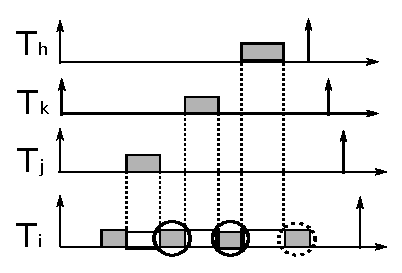
\includegraphics[scale=.65]{figures/figure6-a-1}
\label{fig6-a} 
}\hspace{1cm}
\subfigure[All atomic sections interfere with each other and $s_i^p(\theta)$]{
            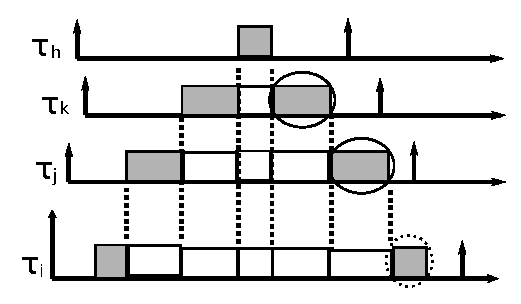
\includegraphics[scale=.6]{figures/figure6-b}
\label{fig6-b} 
}
\begin{tabular}{>{\centering}p{1cm}l}
\includegraphics[scale=0.45]{figures/circle} & Replaced in calculations by $s_{max}(\theta)$\tabularnewline
\includegraphics[scale=0.45]{figures/dotted_circle} & Replaced in calculations by $s_{i_{max}}(\theta)$\tabularnewline
\end{tabular}
\caption{Retry of $s_i^p(\theta)$ due to other atomic sections}  
\label{fig6}
\end{figure*}

\begin{clm}
Claim~\ref{gedf-edf}'s retry bound can be minimized as:
\begin{equation}
RC(T_{i})\le \sum_{\theta\in\theta_{i}}min(\Phi_1 , \Phi_2)\label{eq5}\end{equation}
where $\Phi_1$ is calculated by (\ref{eq3}) for one object $\theta$ (not the sum of objects in $\theta_i$),  and 
\begin{eqnarray}
\Phi_2 & = & \Bigg(\sum_{\tau_{j}\in\gamma_i(\theta)} \Big(\left\lceil\frac{T_{i}}{T_{j}}\right\rceil\sum_{\forall s_{j}^{l}(\theta)}len \big(s_{j}^{l}(\theta)\nonumber \\
 &  & +s_{max}^{*}(\theta) \big) \Big) \Bigg)-\bar{s}_{max}(\theta)+s_{i_{max}}(\theta)\label{eq4}\end{eqnarray}
 where $s^*_{max}$ is the maximum atomic section between all tasks, except $\tau_j$, accessing $\theta$. $\bar{s}_{max}(\theta)$ is the second maximum atomic section between all tasks accessing $\theta$.
\end{clm}
\begin{proof}
(\ref{eq3}) can be modified by noting that a task $\tau_j$'s atomic section 
may conflict with those of other tasks, but not with $\tau_j$. 
This is because, tasks are assumed to arrive sporadically, and  each instance finishes before the next begins. 
Thus, (\ref{eq2}) becomes:
\begin{equation}
W_i^p \left(s_j^k (\theta)\right)\le len\left(s_j^k (\theta)+s^*_{max}(\theta)\right)
\label{eq4-1}\end{equation}

To see why $\bar{s}{}_{max}(\theta)$ is used instead of $s_{max}(\theta)$, the maximum-length atomic section of each task that accesses $\theta$ is grouped into an array, in non-increasing order of their lengths. $s_{max}(\theta)$ will be the first element of this array, and $\bar{s}_{max}(\theta)$ will be the next element, as illustrated in Figure~\ref{fig7}, where the maximum atomic
section of each task that accesses $\theta$ is associated with
its corresponding task. According to (\ref{eq4-1}), all tasks
but $\tau_{j}$ will choose $s_{j_{max}}(\theta)$ as the value of $s_{max}^{*}(\theta)$.
But when $\tau_{j}$ is the one whose contribution is studied,
it will choose $s_{k_{max}}(\theta)$, as it is the maximum one not
associated with $\tau_{j}$. This way, it can be seen that the maximum
value always lies between the two values $s_{jmax}(\theta)$ and $s_{kmax}(\theta)$. 
Of course, these two values can be equal, or the maximum value can be associated with $\tau_i$ itself, and not with any one of the interfering tasks. In the latter case,
the chosen value will always be the one associated with $\tau_i$, which still lies between the two largest values. 

\begin{figure}[htbp]
\centering
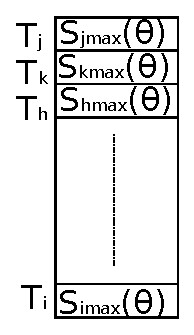
\includegraphics[scale=0.7]{figures/figure7}
\caption{\label{fig7}Values associated with $s_{max}^{*}(\theta)$}
\end{figure}


This means that the subtracted $s_{max}(\theta)$ in (\ref{eq3})
must be replaced with one of these two values ($s_{max}(\theta)$ or $\bar{s}_{max}(\theta)$). However, since we do not know  which task will interfere with $\tau_i$, the minimum is chosen, as we are determining the worst case retry cost (as this value is going to be subtracted),
and this minimum is the second maximum.

Since it is not known a-priori whether $\Phi_1$ will be smaller than $\Phi_2$ for a specific $\theta$, the minimum of $\Phi_1$ and $\Phi_2$ is taken as the worst-case contribution for $\theta$ in $RC(T_i)$. 
%Claim follows.
\end{proof}


\subsection{Upper Bound on Response Time}

To obtain an upper bound on the response time of a task $\tau_{i}$, the term $RC(T_{i})$ must be added to the workload of other tasks during the non-atomic
execution of $\tau_{i}$. But this requires modification of the WCET of each
task as follows. 

$c_{j}$ of each interfering task $\tau_{j}$ should be inflated to accommodate the interference of each task $\tau_{k},$ $k\ne j,i$. Meanwhile, atomic regions that access shared objects between $\tau_{j}$ and $\tau_{i}$ should not be considered in the inflation cost, because they have already been calculated in $\tau_{i}$'s retry cost. Thus, $\tau_{j}$'s inflated WCET becomes:
\begin{equation}
c_{ji}=c_{j}-\left(\sum_{\theta\in(\theta_{j}\wedge\theta_{i})}len \left(s_{j}(\theta) \right) \right)+RC(T_{ji})\label{eq9}\end{equation}
where, $c_{ji}$ is the new WCET of $\tau_{j}$ relative to $\tau_{i}$; 
the sum of lengths of all atomic sections in $\tau_{j}$ that access object $\theta$ is $\sum_{\theta \in (\theta_j \wedge \theta_i)} {len(s_{j}(\theta))}$; and $RC(T_{ji})$ is the $RC(T_j)$ 
 without including the shared objects between $\tau_{i}$ and $\tau_{j}$.
The calculated WCET is relative to task $\tau_{i}$, as it changes from task to task. The upper bound on the response time of $\tau_{i}$, denoted $R_{i}^{up}$, can be calculated iteratively, using a modification of Theorem 6 in~\cite{key-2}, as follows:
\begin{equation}
R_{i}^{up}=c_{i}+RC(T_{i})+\left\lfloor\frac{1}{m}\sum_{j\ne i}W_{ij}(R_{i}^{up})\right\rfloor
\label{eq10}
\end{equation}
where $R_{i}^{up}$'s initial value is $c_{i}+RC(T_{i})$.

$W_{ij}(R_{i}^{up})$ is calculated by (\ref{eq13}), and $W_{ij}(T_{i})$
is calculated by (\ref{eq11}), with $c_{j}$ replaced by 
$c_{ji}$, and changing~(\ref{eq12}) as:
\begin{equation}
W_{ij}(L)=max\begin{cases}
\left(\left\lceil\frac{L-\left(c_{ji}+\sum_{\theta\in(\theta_{j}\wedge\theta_{i})}len(s_{j}(\theta))\right)}{T_{j}}\right\rceil+1 \right)c_{ji}\\
\left\lceil\frac{L-c_{j}}{T_{j}}\right\rceil.c_{ji}+c_{j}-\sum_{\theta\in(\theta_{j}\wedge\theta_{i})}len(s_{j}(\theta))\end{cases}\label{eq14}\end{equation}

(\ref{eq14}) compares two terms, as we have two cases:


\textit{Case 1}. $\tau_j^1$ (shown in Figure~\ref{fig2}) contributes by $c_{ji}$. Thus, other instances of $\tau_j$ will begin after this modified WCET, but the sum of the shared objects' atomic section lengths is removed from $c_{ji}$, causing other instances to start earlier. Thus, the term $\sum_{\theta\in(\theta_i\wedge\theta_j)} {len(s_{j}(\theta))}$ is added to $c_{ji}$ to obtain the correct start time. 

\textit{Case 2}. $\tau_j^1$ contributes by its $c_j$, but the sum of the shared atomic section lengths  between $\tau_i$ and $\tau_j$ should be subtracted from the contribution of $\tau_j^1$, as they are already included in the retry cost. 

It should be noted that subtraction of the sum of the shared objects' atomic section lengths is done in the first case to obtain the correct start time of other instances, while in the second case, this is done to get the correct contribution of $\tau_j^1$. The maximum is chosen from the two terms in (\ref{eq14}), because they differ in the contribution of their $\tau_j^1$s, and the number of instances after that.


\subsubsection{Tighter Upper Bound}

To tighten $\tau_{i}$'s response time upper bound, $RC(\tau_i)$ needs to be calculated recursively over duration $R_i^{up}$, 
and not directly over $T_i$, as done in (\ref{eq10}). So, (\ref{eq5}) must be changed to include the modified number of interfering instances. And if $R_i^{up}$ still extends to $T_i$, a situation like that shown in Figure
\ref{fig10} can happen.
\begin{figure}
\centering{}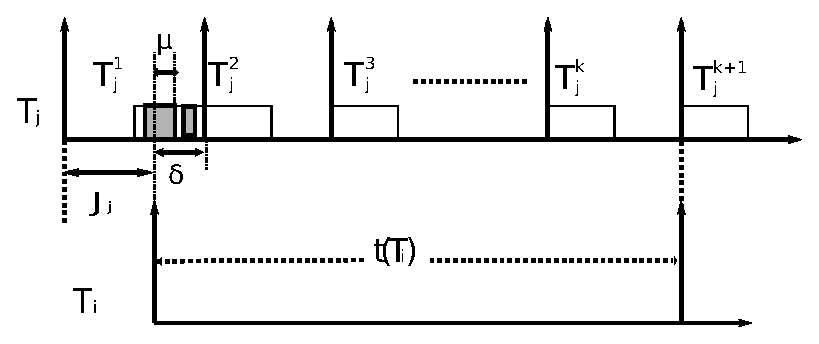
\includegraphics[scale=0.5]{figures/figure10}\caption{\label{fig10} Atomic sections of job $\tau_{j}^{1}$ contributing to period $T_i$}
\end{figure}


To counter the situation in Figure~\ref{fig10}, atomic sections of $\tau_{j}^{1}$ that are contained in the interval $\delta$
are the only ones that can contribute to $RC(T_{i})$. Of course, they can be lower, but cannot be greater, because $\tau_{j}^{1}$ has been delayed by its maximum jitter. Hence, no more atomic sections
can interfere during the duration 
$[d_j^1 -\delta,d_j^1]$.

For simplicity, we use the following notations:
\begin{compactitem}
\item $\lambda_{1}\left(j,\theta\right)=\sum_{\forall s_{j}^{l}\left(\theta\right)\in\left[d_j^1-\delta,d_j^1\right]}len\left(s_{j}^{l^{*}}\left(\theta\right)+s_{max}\left(\theta\right)\right)$
\item $\chi_{1}\left(i,j,\theta\right)=\left\lfloor\frac{T_{i}}{T_{j}}\right\rfloor\sum_{\forall s_{j}^{l}\left(\theta\right)}len\left(s_{j}^{l}\left(\theta\right)+s_{max}\left(\theta\right)\right)$
\item $\lambda_{2}\left(j,\theta\right)=\sum_{\forall s_{j}^{l}\left(\theta\right)\in\left[d_{j}^{1}-\delta,d_{j}^{1}\right]}len\left(s_{j}^{l^{*}}\left(\theta\right)+s_{max}^{*}\left(\theta\right)\right)$
\item $\chi_{2}\left(i,j,\theta\right)=\left\lfloor\frac{T_{i}}{T_{j}}\right\rfloor\sum_{\forall s_{j}^{l}\left(\theta\right)}len\left(s_{j}^{l}\left(\theta\right)+s_{max}^{*}\left(\theta\right)\right)$
\end{compactitem}
Here, $s_{j}^{l^{*}}\left(\theta\right)$ is the part of $s_{j}^{l}\left(\theta\right)$ that
is included in the interval $\delta$. Thus, if $s_j^l (\theta)$ is partially included in $\delta$, it contributes by its included length $\mu$.

Now, (\ref{eq5}) can be modified as:
\begin{equation}
RC\left(T_{i}\right)\le \sum_{\theta\in\theta_{i}}min\begin{cases}
\begin{cases}
\Bigl(\left(\sum_{\tau_{j}\in\gamma_i\left(\theta\right)}\lambda_{1}\left(j,\theta\right)+\chi_{1}\left(i,j,\theta\right)\right)\\
-s_{max}\left(\theta\right)+s_{i_{max}}\left(\theta\right)\Bigr)\end{cases}\\
\begin{cases}
\Bigl(\left(\sum_{\tau_{j}\in\gamma_i\left(\theta\right)}\lambda_{2}\left(j,\theta\right)+\chi_{2}\left(i,j,\theta\right)\right)\\
-\bar{s}_{max}\left(\theta\right)+s_{i_{max}}\left(\theta\right)\Bigr)\end{cases}\end{cases}\label{eq15}\end{equation}



Now, we compute $RC(L)$, where $L$ does not extend to the last instance of $\tau_{j}$. Let:
\begin{compactitem}
\item $\upsilon\left(L,j\right)=\left\lceil\frac{L-c_{j}}{T_{j}}\right\rceil+1$
\item $\lambda_{3}\left(j,\theta\right)=\sum_{\forall s_{j}^{l}\left(\theta\right)}len\left(s_{j}^{l}\left(\theta\right)+s_{max}\left(\theta\right)\right)$
\item $\lambda_{4}\left(j,\theta\right)=\sum_{\forall s_{j}^{l}\left(\theta\right)}len\left(s_{j}^{l}\left(\theta\right)+s_{max}^{*}\left(\theta\right)\right)$
\end{compactitem}
Now, (\ref{eq5}) becomes: 
\begin{equation}
RC\left(L\right)\le \sum_{\theta\in\theta_{i}}min\begin{cases}
\begin{cases}
\left(\sum_{\tau_{j}\in\gamma_i\left(\theta\right)}\left(\upsilon\left(L,j\right)\lambda_{3}\left(j,\theta\right)\right)\right)\\
-s_{max}\left(\theta\right)+s_{i_{max}}\left(\theta\right)\end{cases}\\
\begin{cases}
\left(\sum_{\tau_{j}\in\gamma_i\left(\theta\right)}\left(\upsilon\left(L,j\right)\lambda_{4}\left(j,\theta\right)\right)\right)\\
-\bar{s}_{max}\left(\theta\right)+s_{i_{max}}\left(\theta\right)\end{cases}\end{cases}\label{eq16}\end{equation}


Thus, an upper bound on $RC(\tau_i)$ is given by:
\begin{equation}
RC(R_{i}^{up})\le min\begin{cases}
RC(R_{i}^{up})\\
RC(T_{i})\end{cases}
\label{eq17}
\end{equation}
where $RC(R_i^{up})$ is calculated by~(\ref{eq16}) if $R_i^{up}$ does not extend to the last interfering instance of $\tau_j$; otherwise, it is calculated by~(\ref{eq15}). The final upper bound on $\tau_{i}$'s response time can be calculated
as in (\ref{eq10}) by replacing $RC(T_{i})$ with
$RC(R_{i}^{up})$.



\section{G-RMA/RMA CM Response Time}
\label{sec:g-rma-rma-cm}

As G-RMA is a fixed priority scheduler,  a task $\tau_{i}$ will be interfered by those tasks with priorities higher than $\tau_{i}$ (i.e., $p_{j}>p_{i}$).  Upon a conflict, the RMA CM will commit the transaction that belongs to the higher priority task. Hereafter, we use \emph{RCM} to refer to a multiprocessor system scheduled by G-RMA and resolves STM conflicts by the RMA CM. RCM is shown in Alogrithm~\ref{rcm_algorithm}.
\begin{algorithm}
\footnotesize{
\LinesNumbered
\KwData{$s_i^k(\theta)\rightarrow$ interfered atomic section. $s_j^l(\theta)\rightarrow$ interfering atomic section}
\KwResult{which atomic section aborts}
\eIf{$T_i < T_j$}
	{$s_j^l(\theta)$ aborts\label{step_sicommits}\;}
	{$s_i^k(\theta)$ aborts\label{step_siaborts}\;}
	}
\caption{RCM}
\label{rcm_algorithm}
\end{algorithm}

\subsection{Maximum Task Interference}

Figure~\ref{fig11} illustrates the maximum interference caused by a task $\tau_{j}$
to a task $\tau_{i}$ under G-RMA. As $\tau_{j}$ is of higher priority than $\tau_{i}$,
$\tau_{j}^{k}$ will interfere with $\tau_{i}$ even if it is not totally
included in $T_{i}$. Unlike the G-EDF case shown in Figure~\ref{fig10}, 
where only the $\delta$ part of $\tau_{j}^{1}$ is considered, in G-RMA,
$\tau_{j}^{k}$ can contribute by the whole $c_{j}$, and all atomic
sections contained in $\tau_{j}^{k}$ must be considered. This is because, in G-EDF, the worst-case pattern releases $\tau_{i}^a$ before $d_{j}^{1}$
by $\delta$ time units, and $\tau_{i}^a$ cannot be interfered before it
is released. But in G-RMA, $\tau_{i}^a$ is already released, and can be
interfered by the whole $\tau_{j}^{k}$, even if this makes it infeasible.


\begin{figure}[htbp]
\centering
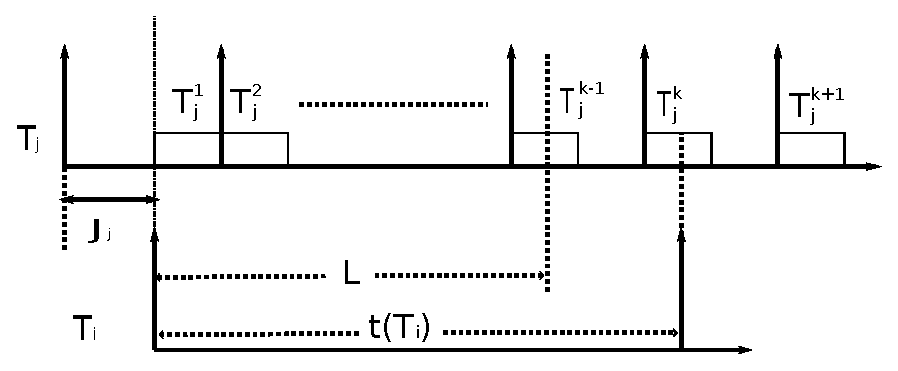
\includegraphics[scale=0.5]{figures/figure11}\caption{\label{fig11}Max interference of $\tau_{j}$ to $\tau_{i}$ in G-RMA}
%%BR: $T_{j}$ and $T_{i}$ are task periods. Is that what you meant here?
\end{figure}

Thus, the maximum contribution of $\tau_{j}^b$ to $\tau_{i}^a$ for any duration
$L$ can be deduced from Figure~\ref{fig11} as $W_{ij}(L)=\left(\left\lceil\frac{L-c_{j}}{T_{j}}\right\rceil+1 \right)c_{j}$,
where $L$ can extend to $T_{i}$. Note the contrast with ECM, where $L$ cannot be extended directly to $T_i$, as this will have a different pattern of worst case interference from other tasks.

\subsection{Retry Cost of Atomic Sections}

\begin{clm}
Under RCM, a task $\tau_i$'s retry cost over duration $L$, which can extend to $T_i$, is upper bounded by:
\begin{eqnarray}
RC\left(L\right) & \le & \sum_{\theta\in\theta_{i}}\Bigg(\left(\sum_{\tau_{j}^{*}}\left(\left(\left\lceil\frac{L-c_{j}}{T_{j}}\right\rceil+1\right)\pi\left(j,\theta\right)\right)\right)\nonumber \\
 & - & s_{max}^{min}\left(\theta\right)+s_{i_{max}}\left(\theta\right)\Bigg)\label{eq20}\end{eqnarray}
 where:
 \begin{compactitem}
\item $\tau_{j}^{*}=\{\tau_{j}|(\tau_{j}\in\gamma_i(\theta))\wedge(p_{j}> p_{i})\}$
\item $\pi(j,\theta)=\sum_{\forall s_{j}^{l}(\theta)}len\left(s_{j}^{l}\left(\theta\right)+s_{max}^{j}\left(\theta\right)\right)$
\item $s_{max}^{min}(\theta)=min_{\forall \tau_j^*} \{s_{max}^j(\theta) \in \tau_k \}$, where $p_j > p_k > p_i$
\end{compactitem}
\end{clm}
\begin{proof}
The worst case interference pattern for RCM is the same as that for ECM for an interval $L$, except that, in RCM, $L$ can extend to the entire $T_i$, but in ECM, it cannot, as the interference pattern of $\tau_j$ to $\tau_i$ changes. 
Thus, (\ref{eq16}) can be used to calculate $\tau_i$'s retry cost, with some modifications, as we do not have to obtain the minimum of the two terms in (\ref{eq16}), because $\tau_j$'s atomic sections will abort and retry only atomic sections of tasks with lower priority than $\tau_j$. Thus, $s_{max}(\theta)$, $s_{max}^*(\theta)$, and $\bar{s}_{max}(\theta)$ are replaced by $s_{max}^{min}(\theta)$, which is the minimum of the set of maximum-length atomic sections of tasks with priority lower than $\tau_j$ and share object $\theta$ with $\tau_i$. This is because, the maximum length atomic section of tasks other than $\tau_j$ differs according to $j$. Besides, as $\tau_i$'s atomic sections can be aborted only by atomic sections of higher priority tasks, not all $\tau_j \in \gamma (\theta)$ are considered, but only the subset of tasks in $\gamma (\theta)$ with priority higher than $\tau_i$ (i.e., $\tau_j^*$). 
Claim follows.
\end{proof}



\subsection{Upper Bound on Response Time}

The response time upper bound can be computed using Theorem 7 in~\cite{key-2} with a modification to include the effect of retry cost. The upper bound is given by:
\begin{equation}
R_{i}^{up}=c_{i}+RC(R_{i}^{up})+\left\lfloor\frac{1}{m}\sum_{j\ne i}W_{ij}(R_{i}^{up})\right\rfloor\label{eq22}\end{equation}
where $W_{ij}(R_{i}^{up})$ is calculated as in (\ref{eq14}), $c_{ji}$ is calculated by (\ref{eq9}), and $RC$ is calculated by (\ref{eq20}).

%%BR: Skipped reviewing the following %%%%%%%%%%%%%
\begin{comment}
\section{FMLP and OMLP Blocking Times}
\label{sec:blocking-bound-fmlp-omlp}

The FMLP protocol~\cite{brandenburg2008comparison} has been shown to be superior to other multiprocessor real-time locking protocols in terms of schedulability, and the global OMLP protocol~\cite{key-3} has been shown to be asymptotically optimal. To formally compare STM against FMLP and global OMLP, we first upper bound their blocking times. %(those were not presented in~\cite{brandenburg2008comparison,key-4,key-3}). 


\subsection{\label{global-fmlp}Global FMLP}

FMLP can be used with global and partitioned scheduling. Since we only consider global scheduling, ``FMLP" and ``global FMLP" mean the same, for the paper's purpose.


FMLP divides shared objects into short resources, $s\_\theta$, and long ones, $l\_\theta$. Nested resources 
are grouped together into two groups: $g(s\_\theta)$ that contains only short resources, and $g(l\_\theta)$ that contains only long resources.
A request $R_i (g(s\_\theta))$ is made by a task $T_i$ to access one or more resources in $g(s\_\theta)$. This request's length is denoted $|R_i (g(s\_\theta))|$, and the number of times $T_i$ requests short resources is denoted $N_{i,s}$. Similarly, $R_i (g(l\_\theta))$ is $T_i$'s request to a group containing long resources for a duration $|R_i (g(l\_\theta))|$, and $N_{i,l}$ is the number of times $T_i$ requests long resources.


Global FMLP uses a variant of G-EDF (called GSN-EDF which discriminates between
linked jobs and scheduled ones) to account for non-preemptive jobs while still using G-EDF for scheduling, 
%%BR: "jobs"?? (can there be multiple linked jobs)?
%%BR: "ones"?? (can there be multiple scheduled ones)?
Tasks busy-wait on short resources, and suspend on long ones. In both cases, requests for resources are arranged in FIFO queues, 
%%BR: "FIFO queue" or "FIFO queues"???? (since there are two resource types)
and for requesting long resources, the task holding the resource inherits the highest priority of the suspended tasks on that resource. For short resources, there is no need to inherit priorities, as tasks become non-preemptable when acquiring short resources. 

Requests for long resources can contain requests for the short resource group, but the reverse is not true. The protocol allows non-preemptable jobs and bounds the time a job is non-preemptively blocked by a lower priority job as the maximum time a non-preemptive section of the job can be linked to the processor of the higher priority job. This non-preemptive blocking can only happen when the higher priority job is released or resumed.


Three types of blocking can be incurred by any task under global FMLP. These include busy-wait blocking, non-preemptive blocking, and direct blocking. The total blocking time of a job, $b_{i}$, is the sum of these three blocking durations. Execution time of each task, $e_{i}$, is inflated by this blocking amount ($e_{i}+b_{i}$), and is used in any of the G-EDF schedulability tests (e.g.,~\cite{Goossens:2003:PSP:876600.876615,srinivasan2002deadline}) 
for verifying schedulability. 

We upper bound a task's blocking durations due to busy-wait blocking, non-preemptive blocking, and direct blocking, denoted as $BW(T_{i})$, $NPB(T_{i})$, and $DB(T_{i})$, respectively, as follows.  
(Note that, in~\cite{key-3}, no upper bounds are presented for these terms, except for $DB(T_{i})$, as~\cite{key-3}'s main focus is on FMLP's suspension-based part. Also, the upper bound for $DB(T_{i})$ in~\cite{key-3} does not consider the effect of requesting a short resource within a long one.)


A job $T_{i}^{j}$ busy-waits in a FIFO queue when it is scheduled on a processor and it cannot be removed by any other task until its request is satisfied. As busy-waiting tasks are non-preemptable, job $T_{i}^{j}$ can be blocked for at most the maximum $m-1$ requests, where each request consists of the sum of the nested requests
to some resources in the same group. This process proceeds for each short resource requested by $T_{i}$. The busy-wait blocking time, $BW(T_{i})$, is therefore:
\begin{equation}
BW(T_{i})\le\sum_{s\_\theta\in\theta_{i}} \left(max \left[\sum_{k=1,k\ne i}^{min(m,n)-1} \left| R_{k} \left(g \left(s\_\theta \right) \right) \right| \right] \right)\label{eq26}
\end{equation}

A job $T_{i}^{j}$ can be non-preemptively blocked, either at its release or when it resumes, by at most the maximum (nested) request to any short resource. The non-preemptive blocking time, $NPB(T_{i})$, is therefore:
\begin{equation}
NPB(T_{i})=(1+N_{i,l}).max_{k\ne i} \left| R_{k}(g(s\_\theta)) \right|\label{eq27}
\end{equation}
Here, $1$ is added to $N_{i,l}$, because $T_{i}$ can be non-preemptively blocked at its release, in addition to suspension times. 

A job $T_{i}^{j}$ can be blocked by all other $n-1$ tasks for any long resource. Any of these $n-1$ requests can be a nested request to long resources belonging to the same group. In addition, any of those requests can contain a request to a short resource, and so it can busy-wait on it. Thus, each request in the $n-1$ requests, requiring access to a short resource, can be delayed by at most the maximum $m-1$ requests to the group containing that short resource. The direct blocking time, $DB(T_{i})$, is therefore:
\begin{equation}
DB(T_{i})\le\sum_{l\_\theta\in\theta_{i}} \left[max_{k=1,k\ne i}^{n-1} \left|R_{k} \left(g \left(l\_\theta \right) \right) \right| \right]
\label{eq28}
\end{equation}


\subsection{Global OMLP}


In~\cite{key-3}, 
global FMLP has a maximum s-oblivious pi-blocking cost of $\Theta(n)$, whereas global OMLP~\cite{key-3}, which is a suspension-based protocol that supports G-EDF, as well as any global job-level static priority (JLSP) scheduler, has a $\Theta(m)$ s-oblivious pi-blocking cost, as seen by equation (\ref{eq29}):
\begin{equation}
b_{i}\triangleq\sum_{k=1}^{q}N_{i,k}.2.(m-1).max_{1\le i\le n}\{L_{i,k}\}\label{eq29}\end{equation}
where $N_{i,k}$ is the maximum number of times $T_i$ requests resource $k$, and $L_{i,k}$ is the maximum execution time of such a request. $N_{i,k}$ and $L_{i,k}$ are assumed to be constants,
so the s-oblivious pi-blocking is $\Theta(m)$, and thus it is optimal.
\end{comment}

%%BR: Resumed editing from here
\section{STM versus Lock-Free}
\label{sec:comparison}

We now would like to understand when STM will be beneficial compared to lock-free synchronization. The retry-loop lock-free approach in~\cite{key-5} is the most relevant to our work. 


\subsection{\label{sub:G-EDF-scheduler-with} ECM versus Lock-Free}

\begin{clm}
For ECM's schedulability to be better or equal to that of~\cite{key-5}'s retry-loop lock-free approach,  
the size of $s_{max}$ must not exceed one half of that of $r_{max}$, where $r_{max}$ is the maximum execution cost of a single iteration of any lock-free retry loop of any task. With low number of conflicting tasks, the size of $s_{max}$ can be at most the size of $r_{max}$. 
\end{clm}
\begin{proof}
Equation (\ref{eq17}) can be upper bounded as:
\begin{equation}
RC\left(T_{i}\right) \le \sum_{\tau_{j}\in\gamma_{i}}\left(\sum_{\theta\in\theta_{i}}\left(\left\lceil\frac{T_{i}}{T_{j}}\right\rceil\sum_{\forall s_{j}^{l}\left(\theta\right)}\left(2.s_{max}\right)\right)\right)
\label{eq30}
\end{equation}
where $s_{j}^{l}\left(\theta\right)$, $s_{i_{max}}\left(\theta\right)$,
$s_{max}^{*}\left(\theta\right)$, and $\bar{s}_{max}\left(\theta\right)$ are replaced by $s_{max}$, and the order of the first two summations are reversed
by each other, 
with $\gamma_{i}$ being the set of tasks that share objects
with $\tau_{i}$. These changes are done to simplify the comparison.

Let $\sum_{\theta\in\theta_{i}}\sum_{\forall s_{j}^{l}\left(\theta\right)}=\beta_{i,j}^{*}$, and $\alpha_{edf}=\sum_{\tau_{j}\in\gamma_{i}}\left\lceil\frac{T_{i}}{T_{j}}\right\rceil.2\beta_{i,j}^*$. Now, (\ref{eq30}) can be modified as:
\begin{equation}
RC\left(T_{i}\right)=\alpha_{edf}.s_{max}
\label{eq31}
\end{equation}

The loop retry cost is given by:
\begin{eqnarray}
LRC\left(T_i\right)&=&\sum_{\tau_{j}\in\gamma_{i}}\left(\left\lceil\frac{T_{i}}{T_{j}}\right\rceil+1\right).\beta_{i,j}.r_{max}\nonumber \\
&=& \alpha_{free} . r_{max} \label{eq32}
\end{eqnarray}
where $\beta_{i,j}$ is the number of retry loops of $\tau_{j}$ that accesses the same object as that accessed by some retry loop of $\tau_{i}$, and $\alpha_{free} = \sum_{\tau_{j}\in\gamma_{i}}\left(\left\lceil\frac{T_{i}}{T_{j}}\right\rceil + 1 \right).\beta_{i,j}$.
Since the shared objects are the same in both STM and lock free, $\beta_{i,j}=\beta_{i,j}^{*}$.
Thus, STM achieves equal or better schedulability 
than lock-free if the total utilization of the STM system is less than or equal to that of the lock-free system:
\begin{eqnarray}
\sum_{\tau_{i}}\frac{c_{i}+\alpha_{edf}.s_{max}} {T_{i}} & \le & \sum_{\tau_{i}}\frac{c_{i}+\alpha_{free}.r_{max}}{T_{i}} \nonumber \\
\therefore\frac{s_{max}}{r_{max}} & \le & \frac{\sum_{\tau_{i}}\alpha_{free}/T_{i}}{\sum_{\tau_{i}}\alpha_{edf}/T_{i}}\end{eqnarray}


Let $\bar{\alpha}_{free}=\sum_{\tau_{j}\in\gamma_{i}}\left\lceil\frac{T_{i}}{T_{j}}\right\rceil.\beta_{i,j}$,  $\hat{\alpha}_{free}=\sum_{T_{j}\in\gamma_{i}}\beta_{i,j}$, and $\alpha_{free}=\bar{\alpha}_{free}+\hat{\alpha}_{free}.$ Therefore: 
\begin{eqnarray}
\frac{s_{max}}{r_{max}} & \le & \frac{\sum_{\tau_{i}}(\bar{\alpha}_{free} +\hat{\alpha}_{free})/T_{i}}{\sum_{\tau_{i}}\alpha_{edf}/T_{i}}\nonumber \\
 & = & \frac{1}{2}+\frac{\sum_{\tau_{i}}\hat{\alpha}_{free} /T_{i}}{\sum_{\tau_{i}}\alpha_{edf}/T_{i}}
 \label{eq33}
 \end{eqnarray}

Let $\zeta_{1}=\sum_{\tau_{i}}\hat{\alpha}_{free}/T_{i}$
and $\zeta_{2}=\sum_{\tau_{i}}\left(\frac{\alpha_{edf}}{2}\right)/T_{i}$. The maximum value of $\frac{\zeta_{1}}{2.\zeta_{2}}=\frac{1}{2}$, which can happen if $T_{j}\ge T_{i}\,\therefore\left\lceil\frac{T_{i}}{T_{j}}\right\rceil=1$. Then $(\ref{eq33})=1$, which is its maximum value. $T_{j}\ge T_{i}$ means that there is a small number of interferences from other tasks
to $\tau_{i}$, and thus low number of conflicts. Therefore, $s_{max}$ is
allowed to be as large as $r_{max}$.

The theoretical minimum value for $\frac{\zeta_{1}}{2.\zeta_{2}}$
is $0$, which can be asymptotically reached if $T_{j}\ll T_{i}$,
$\therefore\,\left\lceil\frac{T_{i}}{T_{j}}\right\rceil\rightarrow\infty$
and $\zeta_{2}\rightarrow\infty$. Thus, $(\ref{eq33})\rightarrow1/2$.

$\beta_{i,j}$ has little effect on $s_{max}/r_{max}$, 
as it is contained in both the numerator and denominator. Irrespective of whether $\beta_{i,j}$ is going to reach its maximum or minimum value, both can be considered constants, and thus removed from (\ref{eq33})'s numerator and denominator. 
However, the number of
interferences of other tasks to $\tau_{i}$, $\left\lceil\frac{T_{i}}{T_{j}}\right\rceil$,
has the main effect on $s_{max}/r_{max}$. This is illustrated in Figure~\ref{fig14}. Claim follows.
\end{proof}

\begin{figure}
\begin{centering}
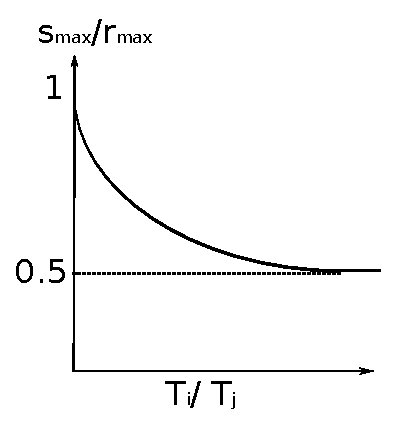
\includegraphics[scale=0.5]{figures/figure14}
\par\end{centering}
\caption{\label{fig14}Effect of $\left\lceil\frac{T_{i}}{T_{j}}\right\rceil$ on
$\frac{s_{max}}{r_{max}}$}
\end{figure}

%%BR: Stopped here. 3:32PM, 10/18/11.

\subsection{RCM versus Lock-Free}

\begin{clm}
For RCM's schedulability to be better or equal to that of~\cite{key-5}'s retry-loop lock-free approach, the size of $s_{max}$ must not exceed one half of that of $r_{max}$ for all cases.
However, the size of $s_{max}$ can be larger than that of $r_{max}$, depending on the number of accesses to a task $T_i$'s shared objects from other tasks.
\end{clm}
\begin{proof}
Equation (\ref{eq20}) is upper bounded by:
 \begin{equation}
\sum_{\left(\tau_{j}\in\gamma_{i}\right)\wedge\left(p_{j}> p_{i}\right)}\left(\left\lceil\frac{T_{i}-c_{j}}{T_{j}}\right\rceil+1\right).2.\beta_{i,j}.s_{max}
\label{eq34}\end{equation}

Consider the same assumptions as in Section~\ref{sub:G-EDF-scheduler-with}.
Let $\alpha_{rma}=\sum_{\left(\tau_{j}\in\gamma_{i}\right)\wedge\left(p_{j}> p_{i}\right)}\left(\left\lceil\frac{T_{i}-c_{j}}{T_{j}}\right\rceil+1\right).2.\beta_{i,j}$. Now, the ratio $s_{max}/r_{max}$ is upper bounded by:
\begin{equation}
\frac{s_{max}}{r_{max}}\le\frac{\sum_{T_{i}}\alpha_{free}/t\left(T_{i}\right)}{\sum_{T_{i}}\alpha_{rma}/t\left(T_{i}\right)}
\label{eq35}\end{equation}

The main difference between RCM and lock-free is that RCM is affected only by the higher priority tasks, while lock-free is affected by all tasks (just as in ECM). 
Besides, RCM
is still affected by $2.\beta_{i,j}$ (just as in ECM).
The subtraction of $c_{j}$ in the numerator of (\ref{eq34}) may not
have a significant effect on the ratio of (\ref{eq35}), as the loop retry 
cost can also be modified to account for the effect of the first interfering
instance of task $T_{j}$. Therefore, 
$\alpha_{free} = \sum_{\tau_{j}\in\gamma_{i}}\left(\left\lceil\frac{T_{i}-c_j}{T_{j}}\right\rceil + 1 \right)\beta_{i,j}$.

Let tasks in the denominator of (\ref{eq35}) be given indexes $k$ instead of $i$, and $l$ instead of $j$. Let tasks in both the numerator and denominator of (\ref{eq35}) be arranged in the non-increasing priority order, so that $i=k$ and $j=l$. Let $\alpha_{free}$ in (\ref{eq35}) be divided into two parts: $\bar{\alpha}_{free}$ that contains only tasks with priority higher than $\tau_i$, and $\hat{\alpha}_{free}$ that contains only tasks with priority lower than $\tau_i$. Now, (\ref{eq35}) becomes:
\begin{eqnarray}
\frac{s_{max}}{r_{max}} & \le & \frac{\sum_{\tau_{i}}(\bar{\alpha}_{free}+\hat{\alpha}_{free})/T_{i}}{\sum_{\tau_{k}}\alpha_{rma}/T_{k}}\nonumber \\
 & = & \frac{1}{2}+\frac{\sum_{\tau_{i}}\hat{\alpha}_{free}/T_{i}}{\sum_{\tau_{k}}\alpha_{rma}/T_{k}}\label{eq36}\end{eqnarray}

For convenience, we introduce the following notations:
\begin{eqnarray}
\zeta_{1}& = & \sum_{\tau_{i}}\frac{\sum_{\left(\tau_{j}\in\gamma_{i}\right)\wedge\left(p_{j}<p_{i}\right)}\left(\left\lceil\frac{T_{i}-c_{j}}{T_{j}}\right\rceil+1\right)\beta_{i,j}}{T_{i}}\nonumber\\
& = & \sum_{T_i} \hat{\alpha}_{free}/T_i
\nonumber\\
\zeta_{2} 
& = & \sum_{\tau_{k}}\frac{\sum_{\left(\tau_{l}\in\gamma_{k}\right)\wedge\left(p_{l}>p_{k}\right)}\left(\left\lceil\frac{T_{k}-c_{l}}{T_{l}}\right\rceil+1\right)\beta_{k,l}}{T_{k}}\nonumber\\
& = & \frac{1}{2}\sum_{\tau_k} \alpha_{rma}/T_k\nonumber
\end{eqnarray}
$\tau_{j}$ is of lower priority than $\tau_{i}$, which means $D_{j}>D_{i}$. Under G-RMA, this means, $T_{j}>T_{i}$.
Thus, $\left\lceil\frac{T_{i}-c_{j}}{T_{j}}\right\rceil=1$ for
all $\tau_{j}$ and $\zeta_{1}=\sum_{\tau_{i}}(\sum_{(\tau_{j}\in\gamma_{i})\wedge(p_{j}<p_{i})}(2.\beta_{i,j}))/T_{i}$.
Since $\zeta_{1}$ contains all $\tau_{j}$ of lower priority than
$\tau_{i}$ and $\zeta_{2}$ contains all $\tau_{l}$ of higher priority than $\tau_{k}$, 
and tasks are arranged in the non-increasing priority order, then for each $\tau_{i,j}$, there exists $\tau_{k,l}$ such
that $i=l$ and $j=k$. Figure~\ref{fig:matrix-example} illustrates this, where 0 means that the pair $i,j$ 
does not exist in $\zeta_{1}$,
and the pair $k,l$ does not exist in $\zeta_{2}$' (i.e., 
there is no task $\tau_l$ that will interfere with $\tau_k$ in $\zeta_2$), 
and 1 means the opposite. 

\begin{figure}[htbp]
\centering
\begin{tabular}{ccc}
$\begin{array}{cccccc}
 & j & 1 & 2 & \cdots & n\\
i\\
1 &  & 0 & 1 & \cdots & 1\\
2 &  & 0 & 0 & \ddots & \vdots\\
\vdots &  & \vdots & \vdots & \ddots & 1\\
n &  & 0 & 0 & \cdots & 0\end{array}$ &  & $\begin{array}{cccccc}
 & l & 1 & 2 & \cdots & n\\
k\\
1 &  & 0 & 0 & \cdots & 0\\
2 &  & 1 & 0 &  & \vdots\\
\vdots &  & \vdots & \ddots & \ddots & 0\\
n &  & 1 & \cdots & 1 & 0\end{array}$\tabularnewline
\end{tabular}
\caption{\label{fig:matrix-example} Task association for lower priority tasks than $T_i$ and higher priority tasks than $T_k$}
\end{figure}


Thus, it can be seen that both the matrices are transposes of
each other. Consequently, for each $\beta_{i,j}$, there exists $\beta_{k,l}$
such that $i=l$ and $j=k$. But the number of times $\tau_{j}$ accesses
a shared object with $\tau_{i}$ may not be the same as the number of times
$\tau_{i}$ accesses that same object. Thus, $\beta_{i,j}$ does not have
to be the same as $\beta_{k,l}$, even if $i,j$ and $k,l$ are transposes 
of each other. Therefore, we can analyze the behavior of $s_{max}/r_{max}$ based on the three parameters $\beta_{i,j}$, $\beta_{k,l}$, and $\left\lceil\frac{T_{k}-c_{l}}{T_{l}}\right\rceil$.
If $\beta_{i,j}$ is increased so that $\beta_{i,j}\rightarrow\infty$,
$\therefore\,(\ref{eq36})\rightarrow\infty$.
This is because, $\beta_{i,j}$ represents the number of times a lower priority task $\tau_{j}$ accesses 
shared objects with a higher priority task $\tau_{i}$. 
While this number has a greater effect in lock-free, it does not have any effect under RCM, because lower priority tasks do not affect higher priority
ones. Hence, $s_{max}$ is allowed to be much greater than $r_{max}$.

Although the minimum value for $\beta_{i,j}$ is 1, mathematically, if $\beta_{i,j}\rightarrow0$, then (\ref{eq36}) 
 $\rightarrow1/2$.
Here, changing $\beta_{i,j}$ does not affect the retry cost of RCM, but it does affect the retry cost of lock-free, because the contention between tasks is reduced. Thus, $s_{max}$ is reduced in this case to
a little more than half of $r_{max}$ (``a little more''
because the minimum value of $\beta_{i,j}$ is actually 1, not 0).


The change of $s_{max}/r_{max}$ with respect to $\beta_{i,j}$ is illustrated in Figure~\ref{fig15-a}.
If $\beta_{k,l}\rightarrow\infty$, then (\ref{eq36}) $\rightarrow1/2$.
This is because, $\beta_{k,l}$ represents the number of times 
a higher priority task $\tau_{l}$ accesses shared objects with a lower
priority task $\tau_{k}$. Under RCM, this will increase the retry 
cost, thus reducing $s_{max}/r_{max}$. But if $\beta_{k,l}\rightarrow0$, then (\ref{eq36})$\rightarrow\infty$. This is due to the lower contention from a higher priority task $\tau_{l}$ to a lower priority task $\tau_{k}$, which reduces the retry cost under RCM and allows $s_{max}$ to be very large compared with $r_{max}$. Of course, the actual minimum value for $\beta_{k,l}$ is 1, and is illustrated in Figure~\ref{fig15-b}.

%%%%%%

The third parameter that affects $s_{max}/r_{max}$ is $T_{k}/T_{l}$.
If $T_{l}\ll T_{k}$, then $\left\lceil\frac{T_{k}-c_{l}}{T_{l}}\right\rceil\rightarrow\infty$,
and (\ref{eq36}) $\rightarrow1/2$. This is due to a high number
of interferences from a higher priority task $\tau_{l}$ to a lower priority
task $\tau_{k}$, which increases the retry cost under RCM, 
%%BR: WHy don't you say "RCM"? Fix it. 
and consequently reduces $s_{max}/r_{max}$. 

If $T_{l}=T_{k}$ (which is
the maximum value for $T_{l}$ as $D_{l}\le D_{k}$, because
$\tau_{l}$ has a higher priority than $\tau_{k}$), then $\left\lceil\frac{T_{k}-c_{l}}{T_{l}}\right\rceil\rightarrow1$
and $\zeta_2=\sum_{\tau_{k}}\frac{\sum_{\left(\tau_{l}\in\gamma_{k}\right)\wedge\left(p_{l}>p_{k}\right)}2\beta_{k,l}}{t_{k}}$. 
This means that the system will be controlled by only two parameters, $\beta_{i,j}$ and $\beta_{k,l}$, as in the previous two cases, illustrated in Figures~\ref{fig15-a} and~\ref{fig15-b}. Claim follows.
\end{proof}

\begin{figure}
\begin{centering}
\subfigure[\label{fig15-a}]{\begin{centering}
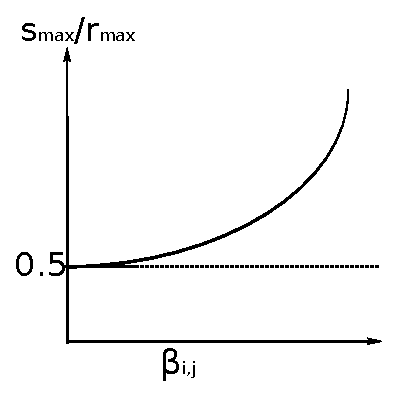
\includegraphics[scale=0.5]{figures/figure15-a}
\par\end{centering}
}\subfigure[\label{fig15-b}]{\begin{centering}
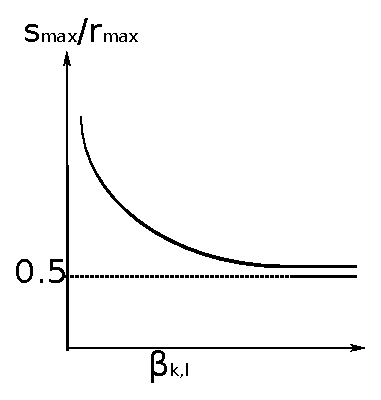
\includegraphics[scale=0.5]{figures/figure15-b}
\par\end{centering}
}
\par\end{centering}
\centering{}\caption{\label{fig15} Change of $s_{max}/r_{max}$: a) $\frac{s_{max}}{r_{max}}$
versus $\beta_{i,j}$ and b) $\frac{s_{max}}{r_{max}}$ versus $\beta_{k,l}$}
\end{figure}


%%BR: Skipped editing from here......
\begin{comment}
\subsection{FMLP \& OMLP versus ECM and RCM
}

\begin{clm}
For ECM's schedulability to be better or equal to that of FMLP or OMLP, 
$s_{max}/|s\_\theta|_{max}$ (in case of FMLP), where $|s\_\theta|_{max}$ be the maximum short request by any task, and $s_{max}/L_{max}$ (in case of OMLP) must  not exceed $O(\frac{m}{n})$, where $L_{max}=max_{\forall i,\forall k}L_{i,k}$. For RCM's schedulability  
to be better or equal  
to that of OMLP, $s_{max}/L_{max}$ must not exceed $O(\frac{m}{n})$.
\end{clm}
\begin{proof}
As FMLP is used with G-EDF (GSN-EDF), we compare only ECM 
against it. 
%%BR: "...we compare only ECM against it."??? 
First, we derive upper bounds for the blocking parameters of FMLP. When requests are non-nested, each resource (short or long) will be contained in its own group. Let $N_{i,s}$ be the number of times a task $T_{i}$ requests a short
resource, $|s\_\theta|_{i,max}$ be the maximum request for a
short resource by $T_{i}$, $\alpha_{bw}=N_{i,s}.(m-1)$. Now, FMLP's three  blocking terms, described in Section~\ref{global-fmlp}, are upper bounded as follows:
\begin{eqnarray*}
BW(T_{i}) & \le & \sum_{s\_\theta\in\theta_{i}}(m-1).|s\_\theta|_{i,max}\\
 & = & N_{i,s}.(m-1).|s\_\theta|_{i,max}\\
 & \le & N_{i,s}.(m-1).|s\_\theta|_{max}\\
& = & \alpha_{bw}.|s\_\theta|_{max}
 \end{eqnarray*}
\begin{eqnarray*}
NPB\left(T_{i}\right) & \le & \left(1+N_{i,l}\right).max\left(BW_{k\ne i}\left(T_{k}\right)+|s\_\theta|_{k,max}\right)\\
 & \le & \left(1+N_{i,l}\right).max\left(BW_{k\ne i}\left(T_{k}\right)+|s\_\theta|_{max}\right)\\
 & = & \left(1+N_{i,l}\right).|s\_\theta|_{max}.max_{k\ne i}\left(N_{k,s}.\left(m-1\right)+1\right)\\
 & = & \alpha_{npb}.|s\_\theta|_{max}
 \end{eqnarray*}
 where $\alpha_{npb}=\left(1+N_{i,l}\right).max_{k\ne i}\left(N_{k,s}.\left(m-1\right)+1\right)$.
\begin{eqnarray*}
DB\left(T_{i}\right) & \le & N_{i,l}.\left(n-1\right).|l\_\theta|_{i,max}\\
 & \le & N_{i,l}.\left(n-1\right).|l\_\theta|_{max}\\
 \end{eqnarray*}
If $|l\_\theta|_{max}\le c1.|s\_\theta|_{max}$, where $c1$ is the
minimum constant that satisfies this relation, then
\begin{eqnarray*}
DB\left(T_{i}\right)& \le & N_{i,l}.\left(n-1\right).c1.|s\_\theta|_{max}\\
& = & \alpha_{db}.|s\_\theta|_{max}
\end{eqnarray*}
where $\alpha_{db}=N_{i,l}.\left(n-1\right).c1$. 

The total blocking time of each task is added to the task execution time, and
as before, we compare the total utilization of the G-EDF system (with both contention managers) against that under FMLP. 

Now, for ECM's schedulability to be better than FMLP,
\begin{equation}
 \frac{s_{max}}{|s\_\theta|_{max}}\le
 \frac{\sum_{T_{i}}\left(\alpha_{bw}+\alpha_{npb}+\alpha_{db}\right) \Big/t(T_{i})}{\sum_{T_{i}}\alpha_{edf} \Big/t(T_{i})}
 \label{eq38} \end{equation}

From (\ref{eq38}), it can be seen that $T_{i}$'s blocking time,
under FMLP, depends on $m,\, n$ and the number of times it requests resources
(in contrast to ECM, 
%%BR: "...contrast to ECM,..."???  
under which, $T_i$'s retry cost depends on the number of times a conflicting task $T_{j}$ requests resources). Thus, if $N_{i,s},\, N_{i,l}$, 
and $N_{k,s}$ can all be upper bounded by some constant $C_{2}$,
which is the maximum number of times any task $T_{i}$ can request a short
or long resource, then the numerator in (\ref{eq38}) 
is $O(n(n+m))$, while the denominator is $O(n^{2})$. Therefore:
\begin{equation}
\frac{s_{max}}{|s\_\theta|_{max}}=O\left(\frac{m}{n} \right)
\label{eq45}
\end{equation}
This means that, for $n<m$, the contention between tasks under both STM and
FMLP is low (even for short resources under FMLP), but FMLP is more affected
by $NTB$. When $n>m$, contention increases, but FMLP arranges
requests in a FIFO queue, so it is less affected than ECM, 
%%BR: "..than ECM,...???
which
suffers from conflicting tasks and instances
of each conflicting one. FMLP is not affected by the number of instances
of each conflicting task.

%%%%
Since OMLP's blocking time is bounded by (\ref{eq29}) \[ \therefore 
%\;
bi\le2.\left(m-1\right).L_{max}\sum_{k=1}^{q}N_{i,k}\]
%%BR: THis sentence is awkward. Why don't you say "Let  \[L_{max}=..... Since OMLP's blocking time is ..., \therefore.."


For ECM's schedulability to be better than global OMLP:
\begin{equation}
\frac{s_{max}}{L_{max}}\le\frac{\sum_{T_{i}}\left(2.\left(m-1\right)\sum_{k=1}^{q}N_{i,k}\right) \Big/t\left(T_{i}\right)}{\sum_{T_{i}}\alpha_{edf} \Big/t\left(T_{i}\right)}\label{eq40}\end{equation}

For RCM, the ratio is:
\begin{equation}
\frac{s_{max}}{L_{max}}\le\frac{\sum_{T_{i}}\left(2.\left(m-1\right)\sum_{k=1}^{q}N_{i,k}\right) \Big/t\left(T_{i}\right)}{\sum_{T_{i}}\alpha_{rma} \big/t\left(T_{i}\right)}\label{eq41}\end{equation}


If $\sum_{k=1}^{q}N_{i,k}$ is upper bounded by $C_{3}$, which is
a constant representing the maximum total number of requests for resources
by any task $T_{i}$, then:
\begin{equation}
\frac{s_{max}}{L_{max}}=O\left(\frac{nm}{n^{2}}\right)=O\left(\frac{m}{n}\right)
\label{eq46}
\end{equation}
for each of (\ref{eq40}) and (\ref{eq41}). Claim follows.
\end{proof}
\end{comment}


%%BR: Re-started editing from here:
\section{Conclusions}
\label{sec:conclusions}

Under both ECM and RCM,  
a task incurs $2.s_{max}$ retry cost for each of its atomic sections due to a conflict with another task's atomic section. Retries under RCM and lock-free are affected by a larger number of conflicting task instances than under ECM. While task retries under ECM and lock-free are affected by all other tasks, retries under RCM are affected only by higher priority tasks. 


STM and lock-free have similar parameters that affect their retry costs---i.e., the number of conflicting jobs and how many times they access shared objects. The $s_{max}/r_{max}$ ratio determines whether STM is better or as good as lock-free. For ECM, this ratio cannot exceed 1, and it can be 1/2 for higher number of conflicting tasks. For RCM, for the common case, $s_{max}$ must be 1/2 of $r_{max}$, and in some cases, $s_{max}$ can be larger than $r_{max}$ by many orders of magnitude.

%The questions that we ask (see Section~\ref{sec:intro}) are fundamentally analytical in nature, and hence, our results are analytical. However, significant insights can be gained by experimental work on a broad range of embedded software, which is outside our work's scope.
\begin{comment}
Our work raises several questions.  
For example, what are the typical range of values for the different parameters that affect the retry cost (and hence the response time)? How tight is our retry and response time bounds in practice? Can real-time CMs be designed for other multiprocessor real-time schedulers (e.g., partitioned, semi-partitioned), and those that dynamically improve application timeliness behavior? These are important directions for further work. 
\end{comment}

%%%%%%%%%%%%%%%%%%%%%%%%%%%%%%%%

\chapter{\label{ch_lcm}LCM}
\markright{Mohammed Elshambakey \hfill Chapter 4. LCM \hfill}

Under ECM and RCM, each atomic section can be aborted for at most $2.s_{max}$ by a single interfering atomic section. We present a novel contention manager (CM) for resolving transactional conflicts, called length-based CM (or LCM). LCM can reduce the abortion time of a single atomic section due to an interfering atomic section below $2.s_{max}$. We upper bound transactional retries and response times under LCM, when used with G-EDF and  G-RMA schedulers. We identify the conditions under which LCM outperforms previous real-time STM CMs and lock-free synchronization. Our implementation and experimental studies reveal that G-EDF/LCM and G-RMA/LCM have shorter or comparable retry costs and response times than other synchronization techniques.

\section{Length-based CM}

LCM resolves conflicts based on the priority of conflicting jobs, besides the length of the interfering atomic section, and the length of the interfered atomic section. This is in contrast to ECM and RCM~\cite{stmconcurrencycontrol:emsoft11}, where conflicts are resolved using the priority of the conflicting jobs. This strategy allows lower priority jobs, under LCM, to retry for lesser time than that under ECM and RCM, but higher priority jobs, sometimes, wait for lower priority ones with bounded priority-inversion.

\subsection{\label{sec 9.1} Design and Rationale}

%Begin algorithm here
\begin{algorithm}
\footnotesize{
\LinesNumbered
\KwData{$s_i^k(\theta)\rightarrow$ interfered atomic section.\\$s_j^l(\theta)\rightarrow$ interfering atomic section.\\$\psi\rightarrow$ predefined threshold $\in [0,1]$.\\$\delta_i^k(\theta)\rightarrow$ remaining execution length of $s_i^k(\theta)$}
\KwResult{which atomic section of $s_i^k(\theta)$ or $s_j^l(\theta)$ aborts}
\eIf{$p_i^k > p_j^l$}
	{$s_j^l(\theta)$ aborts\label{step_sicommits}\;}
	{$c_{ij}^{kl}=len(s_j^l(\theta))/len(s_i^k(\theta))$\label{step_cijkl}\;
	$\alpha_{ij}^{kl}=ln(\psi)/(ln(\psi)-c_{ij}^{kl})$\label{step_alphaijkl}\;
	$\alpha=\left(len(s_i^k(\theta))-\delta_i^k(\theta)\right)/len(s_i^k(\theta))$\;
	\eIf{$\alpha \le \alpha_{ij}^{kl}$}
	{$s_i^k(\theta)$ aborts\label{step_siaborts}\;}
	{$s_j^l(\theta)$ aborts\label{step_sjaborts}\;}
	}
	}
\caption{LCM}
\label{alg_lcm}
\end{algorithm}
%End algorithm here

For both ECM and RCM, $s_{i}^{k}(\theta)$ can be totally repeated if $s_{j}^{l}(\theta)$ --- which belongs to a higher priority job $\tau_{j}^b$ than $\tau_{i}^a$ --- conflicts with $s_{i}^{k}(\theta)$
at the end of its execution, while $s_{i}^{k}(\theta)$ is just about
to commit. Thus, LCM, shown in Algorithm~\ref{alg_lcm}, uses the remaining length of $s_{i}^{k}(\theta)$ when it is interfered,
as well as $len(s_{j}^{l}(\theta))$, to decide which transaction must be aborted. If $p_i^k$ was greater than $p_j^l$, then $s_i^k(\theta)$ would be the one that commits, because it belongs to a higher priority job, and it started before $s_j^l(\theta)$ (step~\ref{step_sicommits}). Otherwise, $c_{ij}^{kl}$ is calculated (step~\ref{step_cijkl}) to determine whether it is worth aborting $s_i^k(\theta)$ in favor of $s_j^l(\theta)$, because $len(s_j^l(\theta))$ is relatively small compared to the remaining execution length of $s_i^k(\theta)$  (explained further).

We assume that:
\begin{equation}
c_{ij}^{kl}=len(s_{j}^{l}(\theta))/len(s_{i}^{k}(\theta))
\label{cm_eq}\end{equation}
where $c_{ij}^{kl}\in]0,\infty[$, to cover all possible lengths of $s_{j}^{l}(\theta)$.
Our idea is to reduce the opportunity for the abort of $s_{i}^{k}(\theta)$ if it is close to committing when interfered and $len(s_{j}^{l}(\theta))$ is large. This abort opportunity is increasingly reduced as $s_{i}^{k}(\theta)$ gets closer to the end of its execution, or $len(s_{j}^{l}(\theta))$ gets larger. 

On the other hand, as $s_{i}^{k}(\theta)$ is interfered early,
or $len(s_{j}^{l}(\theta))$ is small compared to $s_{i}^{k}(\theta)$'s remaining length, the abort opportunity 
is increased even if $s_i^k (\theta)$ is close to the end of its execution. To decide whether $s_{i}^{k}(\theta)$ must be aborted or not, we use a threshold value $\psi\in[0,1]$ that determines $\alpha_{ij}^{kl}$ (step~\ref{step_alphaijkl}), where $\alpha_{ij}^{kl}$ is the maximum percentage of $len(s_i^k(\theta))$ below which $s_j^l(\theta)$ is allowed to abort $s_i^k(\theta)$. Thus, if the already executed part of $s_i^k(\theta)$ --- when $s_j^l(\theta)$ interferes with $s_i^k(\theta)$ --- does not exceed $\alpha_{ij}^{kl}len(s_i^k(\theta))$, then $s_i^k(\theta)$ is aborted (step~\ref{step_siaborts}). Otherwise, $s_j^l(\theta)$ is aborted (step~\ref{step_sjaborts}).

%
\begin{figure}[htbp]
\centering
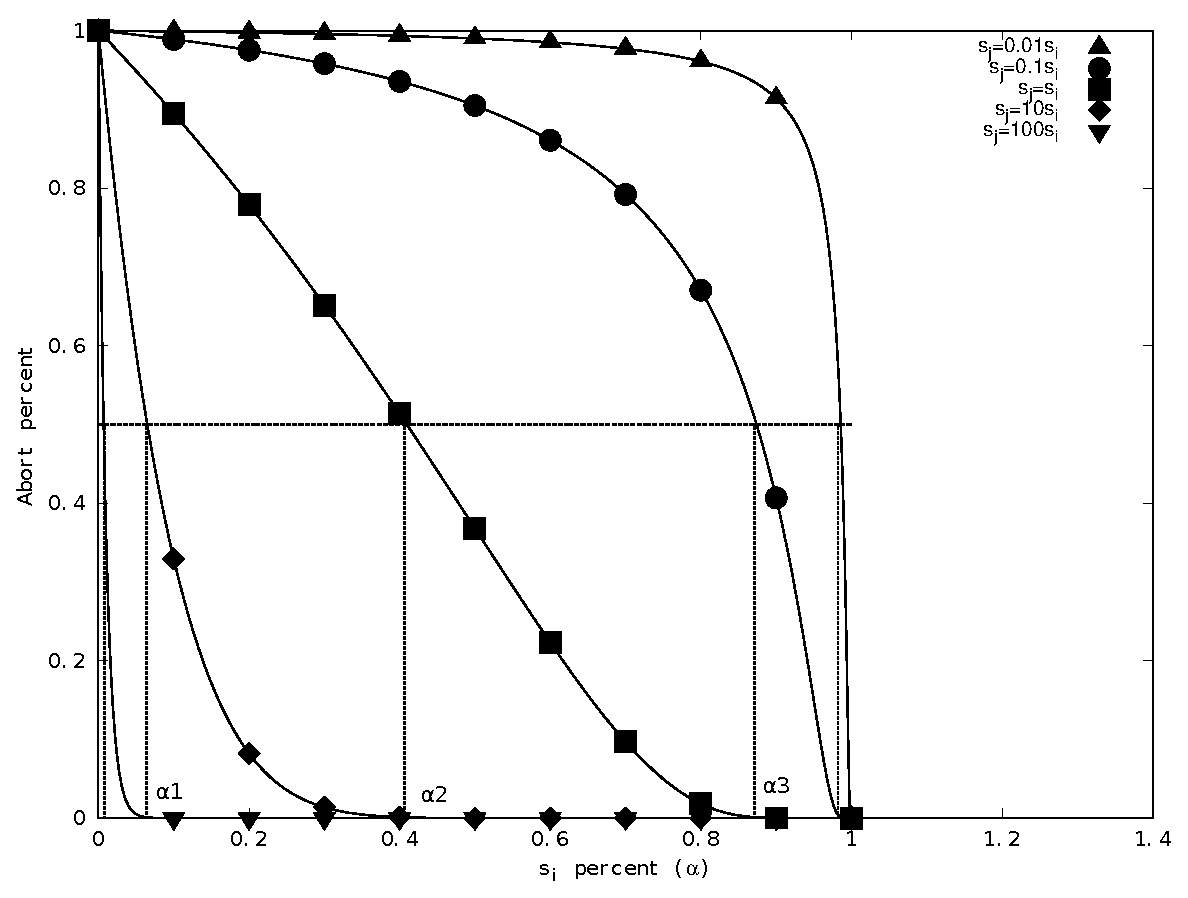
\includegraphics[scale=0.4]{figures/figure16}
\caption{\label{fig16}Interference of $s_{i}^{k}(\theta)$ by various lengths of 
$s_{j}^{l}(\theta)$}
\end{figure}

The behavior of LCM is illustrated in Figure~\ref{fig16}. In this figure, the horizontal axis corresponds to different values of $\alpha$ ranging from $0$ to $1$, and the vertical axis corresponds to different values of abort opportunities, $f(c_{ij}^{kl},\alpha)$, ranging from $0$ to $1$ and calculated by~(\ref{eq49}):
\begin{equation}
f(c_{ij}^{kl},\alpha)=e^{\frac{-c_{ij}^{kl}\alpha}{1-\alpha}}
\label{eq49}\end{equation}
where $c_{ij}^{kl}$ is calculated by~(\ref{cm_eq}).

Figure~\ref{fig16} shows one atomic section $s_i^k(\theta)$ (whose $\alpha$ changes along the horizontal axis) interfered by five different lengths of $s_j^l(\theta)$.
For a predefined value of $f(c_{ij}^{kl},\alpha)$ (denoted as $\psi$ in Algorithm~\ref{alg_lcm}), there corresponds a specific value of $\alpha$ (which is $\alpha_{ij}^{kl}$ in Algorithm~\ref{alg_lcm}) for each curve. For example, when $len(s_j^l(\theta))=0.1 \times len(s_i^k(\theta))$, $s_j^l(\theta)$ aborts $s_i^k(\theta)$ if the latter has not executed more than $\alpha3$ percentage (shown in Figure~\ref{fig16}) of its execution length. As $len(s_{j}^{l}(\theta))$ decreases, the corresponding $\alpha_{ij}^{kl}$ increases (as shown in Figure~\ref{fig16}, $\alpha3>\alpha2>\alpha1$).

Equation (\ref{eq49}) achieves the desired requirement that the abort opportunity is reduced as $s_{i}^{k}(\theta)$ gets
closer to the end of its execution (as $\alpha\rightarrow1,\, f(c_{ij}^{kl},1)\rightarrow0$),
or as the length of the conflicting transaction increases (as $c_{ij}^{kl}\rightarrow\infty,\, f(\infty,\alpha)\rightarrow0$).
Meanwhile, this abort opportunity is increased as $s_{i}^{k}(\theta)$
is interfered closer to its release (as $\alpha\rightarrow0,\, f(c_{ij}^{kl},0)\rightarrow1$),
or as the length of the conflicting transaction decreases (as $c_{ij}^{kl}\rightarrow0,\, f(0,\alpha)\rightarrow1$).

LCM is not a centralized CM, which means that, upon a conflict, each transactions has to decide whether it must commit or abort. 

\begin{clm}
\label{LCM_higher_rc}
Let $s_{j}^{l}(\theta)$ interfere once with $s_{i}^{k}(\theta)$ at $\alpha_{ij}^{kl}$. Then, the maximum contribution of $s_{j}^{l}(\theta)$ to 
$s_{i}^{k}(\theta)$'s 
retry cost is:
\begin{equation}
W_i^k(s_j^l(\theta))\le \alpha_{ij}^{kl}len\Big(s_{i}^{k}(\theta)\Big)+len\Big(s_{j}^{l}(\theta)\Big)\label{eq47}\end{equation}
\end{clm}

\begin{proof}
If $s_{j}^{l}(\theta)$ interferes with $s_{i}^{k}(\theta)$
at a $\Upsilon$ percentage, where $\Upsilon<\alpha_{ij}^{kl}$,
then the retry cost of $s_{i}^{k}(\theta)$ is $\Upsilon len(s_{i}^{k}(\theta))+len(s_{j}^{l}(\theta))$, which is lower than that calculated in (\ref{eq47}). Besides, 
if $s_{j}^{l}(\theta)$ interferes with $s_{i}^{k}(\theta)$ after
$\alpha_{ij}^{kl}$ percentage, then $s_{i}^{k}(\theta)$ will not
abort.
\end{proof}


\begin{clm}
\label{LCM_lower_rc}
An atomic section of a higher priority job, $\tau_{j}^b$, may have to abort and retry due to a lower priority job, $\tau_{i}^a$, if $s_{j}^{l}(\theta)$ interferes
with $s_{i}^{k}(\theta)$ after the $\alpha_{ij}^{kl}$ percentage. $\tau_{j}$'s retry time, due to $s_{i}^{k}(\theta)$ and $s_{j}^{l}(\theta)$,
is upper bounded by:
 \begin{equation}
W_j^l(s_i^k(\theta))\le \Big(1-\alpha_{ij}^{kl}\Big)len\Big(s_{i}^{k}(\theta)\Big)\label{eq48}\end{equation}
\end{clm}

\begin{proof}
It is derived directly from Claim~\ref{LCM_higher_rc}, as $s_j^l(\theta)$ will have to retry for the remaining length of $s_i^k(\theta)$.
\end{proof}

%sh-start
\begin{clm}
\label{no priority inversion in lcm}
A higher priority job, $\tau_i^z$, suffers from priority inversion for at most number of atomic sections in $\tau_i^z$.
\end{clm}

\begin{proof}
Assuming three atomic sections, $s_i^k(\theta)$, $s_j^l(\theta)$ and $s_a^b(\theta)$, where $p_j > p_i$ and $s_j^l(\theta)$ interferes with $s_i^k(\theta)$ after $\alpha_{ij}^{kl}$. Then $s_j^l(\theta)$ will have to abort and retry. At this time, if $s_a^b(\theta)$ interferes with the other two atomic sections, and the LCM decides which transaction to commit based on comparison between each two transactions. So, we have the following cases:-
\begin{itemize}
\item $p_a < p_i < p_j$, then $s_a^b(\theta)$ will not abort any one because it is still in its beginning and it is of the lowest priority. So. $\tau_j$ is not indirectly blocked by $\tau_a$.
\item $p_i<p_a<p_j$ and even if $s_a^b(\theta)$ interferes with $s_i^k(\theta)$ before $\alpha_{ia}^{kb}$, so, $s_a^b(\theta)$ is allowed abort $s_i^k(\theta)$. Comparison between $s_j^l(\theta)$ and $s_a^b(\theta)$ will result in LCM choosing $s_j^l(\theta)$ to commit and abort $s_a^b(\theta)$ because the latter is still beginning, and $\tau_j$ is of higher priority. If $s_a^b(\theta)$ is not allowed to abort $s_i^k(\theta)$, the situation is still the same, because $s_j^l(\theta)$ was already retrying until $s_i^k(\theta)$ finishes.
\item $p_a>p_j>p_i$, then if $s_a^b(\theta)$ is chosen to commit, this is not priority inversion for $\tau_j$ because $\tau_a$ is of higher priority.
\item if $\tau_a$ preempts $\tau_i$, then LCM will compare only between $s_j^l(\theta)$ and $s_a^b(\theta)$. If $p_a<p_j$, then $s_j^l(\theta)$ will commit because of its task's higher priority and $s_a^b(\theta)$ is still at its beginning, otherwise, $s_j^l(\theta)$ will retry, but this will not be priority inversion because $\tau_a$ is already of higher priority than $\tau_j$. If $\tau_a$ does not access any object but it preempts $\tau_i$, then CM will choose $s_j^l(\theta)$ to commit as only already running transactions are competing together.
\end{itemize}
So, by generalizing these cases to any number of conflicting jobs, it is seen that when an atomic section, $s_j^l(\theta)$, of a higher priority job is in conflict with a number of atomic sections belonging to lower priority jobs, $s_j^l(\theta)$ can suffer from priority inversion by only one of them. So, each higher priority job can suffer priority inversion at most its number of atomic section. Claim follows.
\end{proof}

\begin{clm}
\label{max_pri_inv}
The maximum delay suffered by $s_j^l(\theta)$ due to lower priority jobs is caused by the maximum length atomic section accessing object $\theta$, which belongs to a lower priority job than $\tau_j^b$ that owns $s_j^l(\theta)$.
\end{clm}

\begin{proof}
Assume three atomic sections, $s_i^k(\theta)$, $s_j^l(\theta)$, and $s_h^z(\theta)$, where $p_j>p_i$, $p_j>p_h$, and $len(s_i^k(\theta))>len(s_h^z(\theta))$. Now, $\alpha_{ij}^{kl}>\alpha_{hj}^{zl}$ and $c_{ij}^{kl}<c_{hj}^{zl}$. By applying~(\ref{eq48}) to obtain the contribution of $s_i^k(\theta)$ and $s_h^z(\theta)$ to the priority inversion of $s_j^l(\theta)$ and dividing them, we get:
\begin{eqnarray*}
\frac{W_{j}^{l}(s_{i}^{k}(\theta))}{W_{j}^{l}(s_{h}^{z}(\theta))} & = & \frac{\left(1-\alpha_{ij}^{kl}\right)len(s_{i}^{k}(\theta))}{\left(1-\alpha_{hj}^{zl}\right)len(s_{h}^{z}(\theta))}
\end{eqnarray*}
By substitution for $\alpha$s from~(\ref{eq49}):
\begin{eqnarray*}
 & = & \frac{(1-\frac{ln\psi}{ln\psi-c_{ij}^{kl}})len(s_{i}^{k}(\theta))}{(1-\frac{ln\psi}{ln\psi-c_{hj}^{zl}})len(s_{h}^{z}(\theta))}
  =  \frac{(\frac{-c_{ij}^{kl}}{ln\psi-c_{ij}^{kl}})len(s_{i}^{k}(\theta))}{(\frac{-c_{hj}^{zl}}{ln\psi-c_{hj}^{zl}})len(s_{h}^{z}(\theta))}\end{eqnarray*}
$\because ln\psi \le 0$ and $c_{ij}^{kl},c_{hj}^{kl} > 0, \therefore$ by substitution from~(\ref{cm_eq})
\begin{eqnarray*}
 & = & \frac{len(s_{j}^{l}(\theta))/(ln\psi-c_{ij}^{kl})}{len(s_{j}^{l}(\theta))/(ln\psi-c_{hj}^{zl})}
  =  \frac{ln\psi-c_{hj}^{zl}}{ln\psi-c_{ij}^{kl}}>1\end{eqnarray*}
Thus, as the length of the interfered atomic section increases, the delay suffered by the interfering atomic section increases. Claim follows.
\end{proof}


\subsection{\label{response g-edf/lcm} Response Time of G-EDF/LCM}

%Toward establishing the response time under G-EDF/LCM, we introduce a set of Claims.

\begin{clm}\label{GEDF/LCM response time}
$RC(T_i)$ for a task $\tau_i$ under G-EDF/LCM is upper bounded by:
\begin{eqnarray}
RC(T_i) & = & \Bigg(\sum_{\forall \tau_h \in \gamma_i}\sum_{\forall\theta \in \theta_i \wedge \theta_h}\Bigg(\left\lceil\frac{T_{i}}{T_{h}}\right\rceil\sum_{\forall s_{h}^{l}(\theta)}len\Big(s_{h}^{l}(\theta)\Big)\nonumber\\
& + & \alpha_{max}^{hl}len\Big(s_{max}^{h}(\theta)\Big)\Bigg)\Bigg)\nonumber\\
& + & \sum_{\forall s_{i}^{y}(\theta)}\Big(1-\alpha_{max}^{iy}\Big)len\Big(s_{max}^i(\theta)\Big)  
\label{eq78}\end{eqnarray} 
where $\alpha_{max}^{hl}$ is the $\alpha$ value that corresponds to $\psi$ due to the interference of $s_{max}^h(\theta)$ by $s_h^l(\theta)$. $\alpha_{max}^{iy}$ is the $\alpha$ value that corresponds to $\psi$ due to the interference of $s_{max}^i(\theta)$ by $s_i^y(\theta)$.
\end{clm}

\begin{proof}
The maximum number of higher priority instances of $\tau_h$ that can interfere with $\tau_i^x$ is $\left\lceil\frac{T_i}{T_h}\right\rceil$, as shown in Figure~\ref{fig17}, where one instance of $\tau_h$ and $\tau_h^p$ coincides with the absolute deadline of $\tau_i^x$.

By using Claims~\ref{LCM_higher_rc},~\ref{LCM_lower_rc},~\ref{no priority inversion in lcm}, and~\ref{max_pri_inv}, and Claim 1 in~\cite{stmconcurrencycontrol:emsoft11} to determine the effect of atomic sections belonging to higher and lower priority instances of interfering tasks to $\tau_i^x$, Claim follows.
\end{proof}


Response time of $\tau_{i}$ is calculated by (11) in~\cite{stmconcurrencycontrol:emsoft11}.
\begin{figure}
\begin{centering}
\includegraphics[scale=0.6]{figures/figure18}
\par\end{centering}
\caption{\label{fig17}$\tau_h^p$ has a higher priority than $\tau_i^x$}
\end{figure}

\subsection{Schedulability of G-EDF/LCM and ECM}
\label{performance g-edf-lcm}
We now compare the schedulability of G-EDF/LCM with ECM~\cite{stmconcurrencycontrol:emsoft11} %(FMLP and OMLPprotocols~\cite{key-4,brandenburg2008comparison,key-3}), 
to understand when G-EDF/LCM will perform better. 
Toward this, we compare the total utilization of ECM with that of G-EDF/LCM. For each method, we inflate the $c_i$ of each task $\tau_i$ by adding the retry cost suffered by $\tau_i$. Thus, if method $A$ adds retry cost $RC_A(T_i)$ to $c_i$, and method $B$ adds retry cost $RC_B(T_i)$ to $c_i$, then the schedulability of $A$ and $B$ are compared as:
\begin{eqnarray}
\sum_{\forall \tau_{i}}\frac{c_{i}+RC_A(T_{i})}{T_{i}} & \le & \sum_{\forall \tau_{i}}\frac{c_{i}+RC_B(T_{i})}{T_{i}}\nonumber\\
\sum_{\forall \tau_{i}}\frac{RC_A(T_{i})}{T_{i}} & \le & \sum_{\forall \tau_{i}}\frac{RC_B(T_{i})}{T_{i}}
\label{eqa}\end{eqnarray}
Thus, schedulability is compared by substituting the retry cost added by the synchronization methods in (\ref{eqa}).

\begin{clm}\label{lcm versus ecm}
Let $s_{max}$ be the maximum length atomic section accessing any object $\theta$. Let $\alpha_{max}$ and $\alpha_{min}$ be the maximum and minimum values of $\alpha$ for any two atomic sections $s_i^k(\theta)$ and $s_j^l(\theta)$. Given a threshold $\psi$, schedulability of G-EDF/LCM is equal or better than ECM if for any task $\tau_i$:
\begin{equation}
\frac{1-\alpha_{min}}{1-\alpha_{max}} \le \sum_{\forall \tau_h \in \gamma_i}\left\lceil\frac{T_i}{T_h}\right\rceil
\label{edf-lcm-ecm}\end{equation}
\end{clm}

\begin{proof}
Under ECM, $RC(T_{i})$ is upper bounded by:
\begin{equation}
RC(T_{i})\le\sum_{\forall \tau_{h}\in\gamma_{i}}\sum_{\forall \theta\in\ (\theta_{i}\wedge\theta_{h})}\left(\left\lceil\frac{T_{i}}{T_{h}}\right\rceil\sum_{\forall s_{h}^{z}(\theta)}2len(s_{max})\right)\label{eq61}\end{equation}
with the assumption that all lengths of atomic sections of (4) and (8) in~\cite{stmconcurrencycontrol:emsoft11} and~(\ref{eq78}) are replaced by $s_{max}$.
%~\cite{stmconcurrencycontrol:emsoft11}. 
Let $\alpha_{max}^{hl}$ in~(\ref{eq78}) be replaced with $\alpha_{max}$, and $\alpha_{max}^{iy}$ in~(\ref{eq78}) be replaced with $\alpha_{min}$. 
As $\alpha_{max}$, $\alpha_{min}$, and $len(s_{max})$ are all constants, (\ref{eq78}) is upper bounded by:
\begin{eqnarray}
RC(T_i) & \le & \Bigg(\sum_{\forall \tau_h \in \gamma_i}\sum_{\forall\theta \in \theta_i \wedge \theta_h}\Bigg(\left\lceil\frac{T_{i}}{T_{h}}\right\rceil\sum_{\forall s_{h}^{l}(\theta)}\left(1+\alpha_{max}\right)\nonumber\\
& & len\Big(s_{max}\Big)\Bigg)\Bigg)
 +  \sum_{\forall s_{i}^{y}(\theta)}\Big(1-\alpha_{min}\Big)len\Big(s_{max}\Big)\nonumber\\ 
\label{eq101}\end{eqnarray}
%
If $\beta_1^{ih}$ is the total number of times any instance of $\tau_h$ accesses shared objects with $\tau_i$, then $\beta_1^{ih}=\sum_{\forall \theta\in(\theta_{i}\wedge\theta_{h})}\sum_{\forall s_{h}^{z}(\theta)}$. Furthermore, if $\beta_2^i$ is the total number of times any instance of $\tau_i$ accesses shared objects with any other instance,   $\beta_2^i=\sum_{\forall s_{i}^{y}(\theta)}$\textit{, where $\theta$ is shared with another task}. Then, $\beta_{i}=max\{max_{\forall \tau_h \in \gamma_i}\{\beta_1^{ih}\},\beta_2^i\}$ is the maximum number of accesses to all shared objects by any instance of $\tau_{i}$ or $\tau_{h}$. 
Thus, (\ref{eq61}) becomes:
\begin{equation}
RC(T_{i})\le\sum_{\tau_{h}\in\gamma_{i}}2\left\lceil\frac{T_{i}}{T_{h}}\right\rceil\beta_{i}len(s_{max})
\label{eq63}\end{equation}
and (\ref{eq101}) becomes:
\begin{eqnarray}
RC(T_{i}) & \le & \beta_{i}len(s_{max}) \Bigg((1-\alpha_{min})\nonumber\\
& + & \sum_{\forall \tau_h \in \gamma_i}\left\lceil\frac{T_{i}}{T_{h}}\right\rceil(1+\alpha_{max})\Bigg)
\label{eq102}\end{eqnarray}

We can now compare the total utilization of G-EDF/LCM with that of ECM by comparing~(\ref{eq101}) and~(\ref{eq102}) for all $\tau_i$:
\begin{eqnarray}
& & \sum_{\forall \tau_{i}}\frac{(1-\alpha_{min})+\sum_{\forall \tau_{h}\in\gamma_{i}}\left(\left\lceil\frac{T_{i}}{T_{h}}\right\rceil(1+\alpha_{max})\right)}{T_{i}} \nonumber\\
& \le &   \sum_{\forall \tau_{i}}\frac{\sum_{\forall \tau_{h}\in\gamma_{i}}2\left\lceil\frac{T_{i}}{T_{h}}\right\rceil}{T_{i}}\label{eqc}\end{eqnarray}

(\ref{eqc}) is satisfied if for each $\tau_{i}$, the following condition is satisfied:
\begin{equation*}
(1-\alpha_{min})+\sum_{\forall \tau_h \in \gamma_i}\left(\left\lceil\frac{T_{i}}{T_{h}}\right\rceil(1+\alpha_{max})\right)  \le  2\sum_{\forall \tau_h \in \gamma_i}\left\lceil\frac{T_{i}}{T_{h}}\right\rceil
\end{equation*}
\begin{equation*}
\therefore\frac{1-\alpha_{min}}{1-\alpha_{max}}  \le  \sum_{\forall \tau_h \in \gamma_i}\left\lceil\frac{T_{i}}{T_{h}}\right\rceil
\end{equation*}
Claim follows.
\end{proof}


\subsection{G-EDF/LCM versus Lock-free}
\label{gedf-lcm-lock-free}
We consider the retry-loop lock-free synchronization for G-EDF given in~\cite{key-5}. This lock-free approach is the most relevant to our work. 

\begin{clm}\label{gedf-lcm-lock-free_clm} 
Let $s_{max}$ denote $len(s_{max})$ and $r_{max}$ denote the maximum execution cost of a single iteration of any retry loop of any task in the retry-loop lock-free algorithm in~\cite{key-5}. Now, G-EDF/LCM achieves higher schedulability than the retry-loop lock-free approach if the upper bound on $s_{max}/r_{max}$ under G-EDF/LCM ranges between 0.5 and 2 (which is higher than that under  ECM). 
\end{clm}

\begin{proof}
From~\cite{key-5}, the retry-loop lock-free algorithm
is upper bounded by: 
\begin{equation}
RL(T_{i})=\sum_{\tau_{h}\in\gamma_{i}}\left(\left\lceil \frac{T_{i}}{T_{h}}\right\rceil +1\right)\beta_{i}r_{max}\label{eq32-1}
\end{equation}
 where $\beta_{i}$ is as defined in Claim~\ref{lcm versus ecm}.
The retry cost of $\tau_{i}$ in G-EDF/LCM is upper bounded by (\ref{eq102}).
By comparing G-EDF/LCM's total utilization with that of the retry-loop
lock-free algorithm, we get: 
\begin{eqnarray*}
 & \sum_{\forall\tau_{i}}\frac{\left((1-\alpha_{min})+\sum_{\forall\tau_{h}\in\gamma_{i}}\left(\left\lceil \frac{T_{i}}{T_{h}}\right\rceil (1+\alpha_{max})\right)\right)\beta_{i}s_{max}}{T_{i}}\\
\le & \sum_{\forall\tau_{i}}\frac{\sum_{\forall\tau_{h}\in\gamma_{i}}\left(\left\lceil \frac{T_{i}}{T_{h}}\right\rceil +1\right)\beta_{i}r_{max}}{T_{i}}
\end{eqnarray*}
 
\begin{eqnarray}
\therefore\frac{s_{max}}{r_{max}}\le\frac{\sum_{\forall\tau_{i}}\frac{\sum_{\forall\tau_{h}\in\gamma_{i}}\left(\left\lceil \frac{T_{i}}{T_{h}}\right\rceil +1\right)\beta_{i}}{T_{i}}}{\sum_{\forall\tau_{i}}\frac{\left((1-\alpha_{min})+\sum_{\forall\tau_{h}\in\gamma_{i}}\left(\left\lceil \frac{T_{i}}{T_{h}}\right\rceil (1+\alpha_{max})\right)\right)\beta_{i}}{T_{i}}}\label{u-gedf-lcm-ecm}
\end{eqnarray}


Let the number of tasks that have shared objects with $\tau_{i}$
be $\omega$ (i.e., $\sum_{\tau_{h}\in\gamma_{i}}=\omega\ge1$ since
at least one task has a shared object with $\tau_{i}$; otherwise,
there is no conflict between tasks). Let the total number of tasks
be $n$, so $1\le\omega\le n-1$, and $\left\lceil \frac{T_{i}}{T_{h}}\right\rceil \in[1,\infty[$.
To find the minimum and maximum values for the upper bound on $s_{max}/r_{max}$,
we consider the following cases: 
\begin{itemize}
\item $\alpha_{min}\rightarrow0,\alpha_{max}\rightarrow0$ 
\end{itemize}
$\therefore$~(\ref{u-gedf-lcm-ecm}) will be: 
\begin{eqnarray}
\frac{s_{max}}{r_{max}} & \le & 1+\frac{\sum_{\forall\tau_{i}}\frac{\omega-1}{T_{i}}}{\sum_{\forall\tau_{i}}\frac{1+\sum_{\forall\tau_{h}\in\gamma_{i}}\left\lceil \frac{T_{i}}{T_{h}}\right\rceil }{T_{i}}}\nonumber \\
\label{s-r-1}
\end{eqnarray}
 By substituting the edge values for $\omega$ and $\left\lceil \frac{T_{i}}{T_{h}}\right\rceil $
in~(\ref{s-r-1}), we derive that the upper bound on $s_{max}/r_{max}$
lies between 1 and 2.
\begin{itemize}
\item $\alpha_{min}\rightarrow0,\alpha_{max}\rightarrow1$ 
\end{itemize}
(\ref{u-gedf-lcm-ecm}) becomes 
\begin{eqnarray}
\frac{s_{max}}{r_{max}} & \le & 0.5+\frac{\sum_{\forall\tau_{i}}\frac{\omega-0.5}{T_{i}}}{\sum_{\forall\tau_{i}}\frac{1+2\sum_{\forall\tau_{h}\in\gamma_{i}}\left\lceil \frac{T_{i}}{T_{h}}\right\rceil }{T_{i}}}\label{s-r-2}
\end{eqnarray}
 By applying the edge values for $\omega$ and $\left\lceil \frac{T_{i}}{T_{h}}\right\rceil $
in~(\ref{s-r-2}), we derive that the upper bound on $s_{max}/r_{max}$
lies between 0.5 and 1.
\begin{itemize}
\item $\alpha_{min}\rightarrow1,\alpha_{max}\rightarrow0$ 
\end{itemize}
This case is rejected since $\alpha_{min}\le\alpha_{max}$.
\begin{itemize}
\item $\alpha_{min}\rightarrow1,\alpha_{max}\rightarrow1$ 
\end{itemize}
$\therefore$~(\ref{u-gedf-lcm-ecm}) becomes: 
\begin{eqnarray}
\frac{s_{max}}{r_{max}} & \le & 0.5+\frac{\sum_{\tau_{i}}\frac{\omega}{T_{i}}}{2\sum_{\tau_{i}}\frac{\sum_{\forall\tau_{h}\in\gamma_{i}}\left\lceil \frac{T_{i}}{T_{h}}\right\rceil }{T_{i}}}\label{s-r-4}
\end{eqnarray}
 By applying the edge values for $\omega$ and $\left\lceil \frac{T_{i}}{T_{h}}\right\rceil $
in~(\ref{s-r-4}), we derive that the upper bound on $s_{max}/r_{max}$
lies between 0.5 and 1, which is similar to that achieved by ECM.

Summarizing from the previous cases, the upper bound on $s_{max}/r_{max}$
lies between 0.5 and 2, whereas for ECM~\cite{stmconcurrencycontrol:emsoft11},
it lies between 0.5 and 1. Claim follows.

\end{proof}

\subsection{Response Time of G-RMA/LCM}
\label{rma}

\begin{clm}\label{response g-rma/lcm}
Let $\lambda_{2}(j,\theta)=\sum_{\forall s_{j}^{l}(\theta)}len(s_{j}^{l}(\theta))+\alpha_{max}^{jl}len(s_{max}^{j}(\theta))$, where $\alpha_{max}^{jl}$ is the $\alpha$ value corresponding to $\psi$ due to the interference of $s_{max}^j(\theta)$ by $s_j^l(\theta)$. The retry cost of any task $\tau_i$ under G-RMA/LCM during $T_i$ 
is given by:
\begin{eqnarray}
RC\left(T_i\right) & = &
  \sum_{\forall \tau_{j}^{*}}\left(\sum_{\theta\in(\theta_{i}\wedge\theta_{j})}\left(\left(\left\lceil\frac{T_i}{T_{j}}\right\rceil +1\right)\lambda_{2}(j,\theta)\right)\right)\nonumber\\
& + & \sum_{\forall s_{i}^{y}(\theta)}\Big(1-\alpha_{max}^{iy}\Big)len\Big(s_{max}^i(\theta)\Big)
\label{eq60}
\end{eqnarray}
where $\tau_{j}^{*}=\{\tau_{j}|(\tau_{j}\in\gamma_{i})\wedge(p_{j}>p_{i})\}$.
\end{clm}

\begin{proof}
Under G-RMA, all instances of a higher priority task, $\tau_{j}$, can conflict with a lower priority task,
$\tau_{i}$, during $T_{i}$. (\ref{eq47}) can be used to determine the contribution of each conflicting atomic section in $\tau_j$ to $\tau_i$. Meanwhile, all instances of any task with lower priority than $\tau_{i}$ can conflict with $\tau_i$ during $T_{i}$. Claims~\ref{LCM_lower_rc} and~\ref{no priority inversion in lcm} can be used to determine the contribution of conflicting atomic sections in lower priority tasks to $\tau_i$.
%
  %over the whole $t(T_i)$ (unlike the case of G-EDF/LCM, where (\ref{eq59}) chooses which equation to use depending on whether or not $L$ is less than $\left\lfloor\frac{t(T_{i})-c_{h}}{t(T_{h})}\right\rfloor t(T_{h})+c_{h}$).
Using the previous notations and Claim 3 in~\cite{stmconcurrencycontrol:emsoft11}, the Claim follows.
\end{proof}

The response time is calculated by (17) in~\cite{stmconcurrencycontrol:emsoft11} with replacing $RC(R_i^{up})$ with $RC(T_i)$.
%BR: You should say "..with $RC(T_i)$ replacing $RC(R_i^{up})$."

\subsection{Schedulability of G-RMA/LCM and RCM}
\label{rma eval}

\begin{clm}\label{rma_eval_clm}
Under the same assumptions of Claims~\ref{lcm versus ecm} and~\ref{response g-rma/lcm}, G-RMA/LCM's schedulability is equal or better than RCM if:
\begin{equation}
\frac{1-\alpha_{min}}{1-\alpha_{max}}\le \sum_{\forall \tau_j^*}\left( \left\lceil\frac{T_i}{T_j}\right\rceil +1 \right)
\label{eq70}\end{equation}
\end{clm}

\begin{proof}
Under the same assumptions as that of Claims~\ref{lcm versus ecm} and~\ref{response g-rma/lcm}, (\ref{eq60}) can be upper bounded as:
\begin{eqnarray}
RC(T_i) & \le & \sum_{\forall \tau_{j}^{*}}\bigg(\left(\left\lceil\frac{T_{i}}{T_{j}}\right\rceil +1\right)(1+\alpha_{max})
 len(s_{max})\beta_{i}\bigg)\nonumber\\
 & + & (1-\alpha_{min})len(s_{max})\beta_{i}\label{eq68}\end{eqnarray}
 
For RCM, (16) in~\cite{stmconcurrencycontrol:emsoft11} for $RC(T_{i})$ is upper bounded by:
\begin{equation*}
RC(T_{i})\le\sum_{\forall \tau_{j}^{*}}\left(\left\lceil\frac{T_{i}}{T_{j}}\right\rceil +1\right)2\beta_{i}len(s_{max})\label{eq69}\end{equation*}\
By comparing the total utilization of G-RMA/LCM with that of RCM,
we get:
\begin{eqnarray}
 & \sum_{\forall\tau_{i}}\frac{len\left(s_{max}\right)\beta_{i}\left(\left(1-\alpha_{min}\right)+\sum_{\forall\tau_{j}^{*}}\left(\left(\left\lceil\frac{T_{i}}{T_{j}}\right\rceil+1\right)\left(1+\alpha_{max}\right)\right)\right)}{T_{i}}\nonumber\\
\le & \sum_{\forall\tau_{i}}\frac{2len\left(s_{max}\right)\beta_{i}\sum_{\forall\tau_{j}^{*}}\left(\left\lceil\frac{T_{i}}{T_{j}}\right\rceil+1\right)}{T_{i}}\label{grma-lcm-rcm}\end{eqnarray}
(\ref{grma-lcm-rcm}) is satisfied if $\forall \tau_i$~(\ref{eq70}) is satisfied. Claim follows.
\end{proof}


\subsection{G-RMA/LCM versus Lock-free}\label{g-rma lcm vs lock-free}

Although~\cite{key-5} considers retry-loop lock-free synchronization
for G-EDF systems,~\cite{key-5} also applies for G-RMA systems.

\begin{clm}\label{lcm rma lock-free comparison clm}

Let $s_{max}$ denote $len(s_{max})$ and $r_{max}$ denote the maximum
execution cost of a single iteration of any retry loop of any task
in the retry-loop lock-free algorithm in~\cite{key-5}. G-RMA/LCM
achieves higher schedulability than the retry-loop lock-free approach
if the upper bound on $s_{max}/r_{max}$ under G-RMA/LCM is no less
than 0.5. Upper bound on $s_{max}/r_{max}$ can extend to large values
when $\alpha_{min}$ and $\alpha_{max}$ are very large.

\end{clm}

\begin{proof}

The retry cost for G-RMA/LCM is upper bounded by~(\ref{eq60}). Let $\gamma_{i}=\tau_{j}^{*}\cup\bar{\tau_{j}}$,
where $\tau_{j}^{*}$ is the set of higher priority tasks than $\tau_{i}$
sharing objects with $\tau_{i}$. $\bar{\tau_{j}}$ is the set
of lower priority tasks than $\tau_{i}$ sharing objects with
it. We follow the same definitions of $\beta_{i},\, r_{max}$, and
$RL(T_{i})$ given in the proof of Claim (\ref{gedf-lcm-lock-free_clm}).
Schedulability of G-RMA/LCM equals or exceeds the schedulability of retry-loop
lock-free algorithm if:
\begin{eqnarray}
\frac{s_{max}}{r_{max}} & \le & \frac{\sum_{\forall\tau_{i}}\frac{\sum_{\tau_{j}^{*}}\left(\left\lceil \frac{T_{i}}{T_{j}}\right\rceil +1\right)}{T_{i}}}{\sum_{\forall\tau_{i}}\frac{\Big(1-\alpha_{min}\Big)+\sum_{\tau_{j}^{*}}\left(\left\lceil \frac{T_{i}}{T_{j}}\right\rceil +1\right)\left(1+\alpha_{max}\right)}{T_{i}}}\nonumber\\
 & + & \frac{2\sum_{\forall\tau_{i}}\frac{\sum_{\forall\bar{\tau_{j}}}}{T_{i}}}{\sum_{\forall\tau_{i}}\frac{\Big(1-\alpha_{min}\Big)+\sum_{\tau_{j}^{*}}\left(\left\lceil \frac{T_{i}}{T_{j}}\right\rceil +1\right)\left(1+\alpha_{max}\right)}{T_{i}}}\nonumber\\
 & & \label{eq:lcm rma lock-free comparison 1} 
\end{eqnarray}
If $p_{j}<p_{i},\,\therefore\,\left\lceil \frac{T_{i}}{T_{j}}\right\rceil =1$, 
because the system assumes implicit deadline tasks and uses the G-RMA
scheduler. 
%
Let $\omega_{1}$ be the size of $\tau_i^*$ and $\omega_{2}$
be the size of $\bar{\tau_i}$. $\therefore$ $\omega_{1}^{i}\ge 1$ and $\omega_{2}^{i}\ge1$.
Otherwise, there is no conflict with $\tau_{i}$. To find the maximum
and minimum upper bounds for $s_{max}/r_{max}$, the following cases
are considered:
\begin{itemize}
\item $\alpha_{min}\rightarrow0,\,\alpha_{max}\rightarrow0$
\begin{equation}
\therefore\frac{s_{max}}{r_{max}}\le1+\frac{\sum_{\forall\tau_{i}}\frac{2\omega_{2}^{i}-1}{T_{i}}}{\sum_{\forall\tau_{i}}\frac{1+\sum_{\tau_{j}^{*}}\left(\left\lceil \frac{T_{i}}{T_{j}}\right\rceil +1\right)}{T_{i}}}\label{eq:lcm rma lock-free comparison 3}
\end{equation}
As the second term in (\ref{eq:lcm rma lock-free comparison 3}) is
always positive (because $\omega_{2}^{i}\ge1$), the minimum
upper bound on $s_{max}/r_{max}$ is $1$. To get the maximum upper
bound on $s_{max}/r_{max}$, let $\left\lceil \frac{T_{i}}{T_{j}}\right\rceil $
approach its minimum value of $1$, $\omega_{1}^{i}\rightarrow0$, and $\omega_{2}^{i}\rightarrow n-1$ 
(the maximum and minimum values for $\omega_{1}^{i}$ and $\omega_{2}^{i}$, 
respectively. $n$ is number of tasks). Now:
\[
\therefore\frac{s_{max}}{r_{max}}\le\left(2n-2\right)
\]
Of course, $n$ cannot be lower than $2$. Otherwise, there will be
no conflicting tasks.

\item $\alpha_{min}\rightarrow0,\,\alpha_{max}\rightarrow1$
\begin{equation}
\frac{s_{max}}{r_{max}}\le\frac{1}{2}+\frac{\sum_{\forall\tau_{i}}\frac{4\omega_{2}^{i}-1}{T_{i}}}{2\sum_{\forall\tau_{i}}\frac{1+2\sum_{\tau_{j}^{*}}\left(\left\lceil \frac{T_{i}}{T_{j}}\right\rceil +1\right)}{T_{i}}}\label{eq:lcm rma lock-free comparison 4}
\end{equation}
The minimum upper bound for $s_{max}/r_{max}$ is $0.5$. This can
happen when $T_{i}\gg T_{j}$. To get the maximum upper bound on $s_{max}/r_{max}$,
let $\left\lceil \frac{T_{i}}{T_{j}}\right\rceil $ approach its
minimum value $1$, $\omega_{2}^{i}\rightarrow n-1$, and $\omega_{1}^{i}\rightarrow0$. 
Now:
\[
\frac{s_{max}}{r_{max}}\le2n-2
\]

\item $\alpha_{min}\rightarrow1,\,\alpha_{max}\rightarrow0$
This case is rejected because $\alpha_{max}$ must be greater or equal
to $\alpha_{min}$.

\item $\alpha_{min}\rightarrow1,\,\alpha_{max}\rightarrow1$
\begin{equation}
\frac{s_{max}}{r_{max}}\le\frac{1}{2}+\frac{\sum_{\forall\tau_{i}}\frac{\omega_{2}^{i}}{T_{i}}}{\sum_{\forall\tau_{i}}\frac{\sum_{\tau_{j}^{*}}\left(\left\lceil \frac{T_{i}}{T_{j}}\right\rceil +1\right)}{T_{i}}}\label{eq:lcm rma lock-free comparison 5}
\end{equation}
The minimum upper bound for $s_{max}/r_{max}$ is $0.5$. This can
happen when $T_{i}\gg T_{j}$. To get the maximum upper bound on $s_{max}/r_{max}$,
let $\left\lceil \frac{T_{i}}{T_{j}}\right\rceil $ approach its
minimum value $1$, $\omega_{2}^{i}\rightarrow n-1,\,\omega_{1}^{i}\rightarrow0$.
%BR: Again, you may need an "and". 
Now:  
\[
\frac{s_{max}}{r_{max}}\rightarrow\infty
\]

\end{itemize}
From the previous cases, we can derive that the upper bound on $s_{max}/r_{max}$
extends from $0.5$ to large values. Claim follows.
\end{proof}

\section{Conclusions}
\label{sec:conclusions_lcm}

In ECM and RCM, a task incurs at most $2s_{max}$ retry cost for each of its atomic section due to conflict
with another task's atomic section. With LCM, this retry cost is reduced to $(1+\alpha_{max})s_{max}$ for each aborted atomic section. In ECM and RCM, tasks do not retry due to lower priority tasks, whereas in LCM, they do so. In G-EDF/LCM, retry due to a lower priority job is encountered only from a task $\tau_{j}$'s last job instance 
during $\tau_{i}$'s period. This is not the case with G-RMA/LCM, because,  each higher priority task can be aborted and retried by any job instance of lower priority tasks. Schedulability of G-EDF/LCM and G-RMA/LCM is better or equal to ECM and RCM, respectively, by proper choices for $\alpha_{min}$ and $\alpha_{max}$. Schedulability of G-EDF/LCM is better than retry-loop lock-free synchronization for G-EDF if the upper bound on $s_{max}/r_{max}$ is between 0.5 and 2, which is higher than that achieved by ECM. 
G-RMA/LCM achieves higher schedulability than retry-loop lock-free synchronization if $s_{max}/r_{max}$ is not less than 0.5. For high values of $\alpha$ in G-RMA/LCM, $s_{max}/r_{max}$ can extend to large values.

%%%%%%%%%%%%%%%%%%%%%%%%%%%%%%%%

\chapter{\label{ch_pnf}PNF}
\markright{Mohammed Elshambakey \hfill Chapter 5. PNF \hfill}


In this chapter, we present a novel contention manager for resolving transactional conflicts, called PNF. We upper bound transactional retries and task response times under PNF, when used with the G-EDF and  G-RMA schedulers. We formally identify the conditions under which PNF outperforms previous real-time STM contention managers and lock-free synchronization. We also implement PNF and competitor techniques in the Rochester STM framework and conduct experimental studies using a real-time Linux kernel to understand average-case performance. Our work reveals that G-EDF/PNF and G-RMA/PNF have shorter or comparable retry costs than other synchronization techniques.

\section{ECM, RCM and LCM: Limitations}\label{probelm description}

ECM and RCM~\cite{stmconcurrencycontrol:emsoft11} use dynamic and fixed priorities, respectively, to resolve transactional conflicts. ECM is used with the G-EDF scheduler, and allows the transaction whose job has the earliest absolute deadline to commit first~\cite{6045438}. RCM is used with the G-RMA scheduler, and allows the transaction whose job has the shortest relative deadline to commit first.

G-EDF/LCM~\cite{lcmdac2012} and G-RMA/LCM act as ECM and RCM respectively with some difference. Under LCM, higher priority transaction $s_i^k(\theta)$ cannot abort a lower priority transaction $s_j^l(\theta)$ if $s_j^l(\theta)$ has already passed $\alpha$ percentage of its length.

As mentioned before, \cite{stmconcurrencycontrol:emsoft11,lcmdac2012} assumes that each transaction accesses only one object. This assumption simplifies the retry cost (Claims 2 and 3 in~\cite{stmconcurrencycontrol:emsoft11}, and Claims 5, 8 in~\cite{lcmdac2012}) and response time analysis (Sections 4 and 5 in~\cite{stmconcurrencycontrol:emsoft11}, and Sections 4.2, 4.5 in~\cite{lcmdac2012}). Besides, it enables a one-to-one comparison with lock-free synchronization in~\cite{key-5}. With multiple objects per transaction, \cite{stmconcurrencycontrol:emsoft11} and~\cite{lcmdac2012} will introduce transitive retry, which we illustrate with an example.

\textbf{Example 1.} Consider three atomic sections $s_{1}^{x}$, $s_{2}^{y}$, 
and $s_{3}^{z}$ belonging to jobs $\tau_{1}^{x}$,$\tau_{2}^{y}$, 
and $\tau_{3}^{z}$, with priorities $p_{3}^{z}>p_{2}^{y}>p_{1}^{x}$, respectively. 
Assume that $s_{1}^{x}$ and $s_{2}^{y}$ share objects, $s_{2}^{y}$ and $s_{3}^{z}$
share objects. $s_{1}^{x}$ and $s_{3}^{z}$ do not share objects.
$s_{3}^{z}$ can cause $s_{2}^{y}$ to retry, which in turn will cause $s_{1}^{x}$ to retry. 
This means that $s_{1}^{x}$ may retry transitively
because of $s_{3}^{z}$, which will increase the retry cost of $s_{1}^{x}$.

Assume another atomic section $s_4^f$ is introduced. Priority of $s_4^f$ is higher than priority of $s_3^z$. $s_4^f$ shares objects only with $s_3^z$. Thus, $s_4^f$ can make $s_3^z$ to retry, which in turn will make $s_2^y$ to retry, and finally, $s_1^x$ to retry. Thus, transitive retry will move from $s_{4}^{f}$ to $s_{1}^{x}$, increasing the retry cost of $s_{1}^{x}$. 
The situation gets worse as more tasks of higher priorities are added, where each task
shares objects with its immediate lower priority task. $\tau_{3}^{z}$
may have atomic sections that share objects with $\tau_{1}^{x}$,
but this will not prevent the effect of transitive retry due to $s_{1}^{x}$.

\begin{mydef}
\textbf{Transitive Retry:} A transaction $s_{i}^{k}$ suffers from
transitive retry when it conflicts with a higher priority transaction
$s_{j}^{l}$, which in turn conflicts with a higher priority transaction
$s_{z}^{h}$, but $s_{i}^{k}$ does not conflict with $s_{z}^{h}$.
Still, when $s_{j}^{l}$ retries due to $s_{z}^{h}$, $s_{i}^{k}$
also retries due to $s_{j}^{l}$. Thus, the effect of the higher priority
transaction $s_{z}^{h}$ is transitively moved to the lower priority
transaction $s_{i}^{k}$, even when they do not conflict on common objects.
\end{mydef}

\begin{clm}\label{ecm-rcm-transitive-retry}
ECM, RCM and LCM suffer from transitive retry for multi-object transactions.
\end{clm}
\begin{proof}
ECM, RCM and LCM depend on priorities to resolve conflicts between transactions. Thus, lower priority transaction must always be aborted for a conflicting higher priority transaction in ECM and RCM. In LCM, lower priority transactions are conditionally aborted for higher priority ones. Claim follows. 
\end{proof}

Therefore, the analysis in~\cite{stmconcurrencycontrol:emsoft11} and~\cite{lcmdac2012} must extend the set of objects that can cause an atomic section of a lower priority job to retry.  This can be done by initializing the set of conflicting objects, $\gamma_i$, to all objects accessed by all transactions of $\tau_i$. We then cycle through all transactions belonging to all other higher priority tasks. Each transaction $s_j^l$ that accesses at least one of the objects in $\gamma_i$ adds all other objects accessed by $s_j^l$ to $\gamma_i$. The loop over all higher priority tasks is repeated, each time with the new $\gamma_i$, until there are no more transactions accessing any object in $\gamma_i$\footnote{However, note that, this solution may over-extend the set of conflicting objects, and may even contain all objects accessed by all tasks.}.

In addition to the \emph{transitive retry} problem, retrying higher priority transactions can prevent lower priority tasks from running. This happens when all processors are busy with higher priority jobs. When a transaction retries, the processor time is wasted. Thus, it would be better to give the processor to some other task.


Essentially, what we present is a new contention manager that avoids the effect of transitive retry. We call it, Priority contention manager with Negative values and First access (or PNF). PNF also tries to enhance processor utilization. This is done by allocating processors to jobs with non-retrying transactions. PNF is described in detail in Section \ref{PNF}.

\section{The PNF Contention Manager\label{PNF}}

\begin{algorithm}
\footnotesize{
\LinesNumbered
\KwData{
\textit{Executing Transaction:} is one that cannot be aborted by any other transaction, nor preempted by a higher priority task\;
\textit{$m$-set:} $m$-length set that contains only non-conflicting executing transactions\;
\textit{$n$-set:} $n$-length set that contains retrying transactions for $n$ tasks in non-increasing order of priority\;
\textit{n(z):} transaction at index $z$ of the $n$-set\;
$s_i^k$: a newly released transaction\;
$s_j^l$: one of the executing transactions\;
}
\KwResult{atomic sections that will commit}
\eIf{$s_i^k$ does not conflict with any executing transaction\label{s_i^k true}}
{
Assign $s_i^k$ as an executing transaction\;
Add $s_i^k$ to the $m$-set\;
Select $s_i^k$ to commit
}
{
Add $s_i^k$ to the $n$-set according to its priority\label{move to n}\;
Assign temporary priority -1 to the job that owns $s_i^k$ \label{priority to -1}\;
Select transaction(s) conflicting with $s_i^k$ for commit\label{s_i^k commit}\;
}
\If{$s_j^l$ commits\label{s_j^l commits}}
{
	\For{z=1 to size of n-set\label{traverse n-set}}
	{
		\If{n(z) does not conflict with any executing transaction\label{n(z) no conflict}}
		{
			\If{processor available\label{processor available}}
			{
				Restore priority of task owning n(z)\;
				Assign n(z) as executing transaction\;
				Add n(z) to m-set\;
				Select n(z) for commit\;
			}
		}
		move to the next n(z)\;
	}
}
}
\caption{PNF Algorithm} \label{PNF-algorithm}
\end{algorithm}

Algorithm \ref{PNF-algorithm} describes PNF. It
manages two sets. The first is the $m$-set, which contains at most $m$ non-conflicting
transactions, where $m$ is the number of processors, as
there cannot be more than $m$ executing transactions (or generally,
$m$ executing jobs) at the same time. When a transaction is entered
in the $m$-set, it executes non-preemptively and no other transaction
can abort it. A transaction in the $m$-set is called an \emph{executing
transaction}. 
This means that, when a transaction is executing before
the arrival of higher priority conflicting transactions, then the
one that started executing first will be committed (Step~\ref{s_i^k commit}) (hence the word ``First'' in the algorithm's name). 

The second set is the $n$-set, which holds the transactions
that are retrying because of a conflict with one or more of the executing
transactions (Step~\ref{move to n}), where $n$ stands for
the number of tasks in the system. It also holds transactions that
cannot currently execute, because processors are busy, either due to processing preempted transaction
and/or higher priority jobs. Any transaction in the $n$-set is assigned a temporal
priority of -1 (Step~\ref{priority to -1}) (hence the word 
``Negative'' in the algorithm's name). A negative priority
is considered smaller than any normal priority, and a transaction
continues to hold this negative priority until it is moved to the $m$-set, where it is restored its normal priority.


A job holding a transaction in the $n$-set can be preempted by any other job with normal priority, even if that normal priority job does not have transactions conflicting with the preempted job. Hence, this set is of length $n$, as there can be at most $n$ jobs in the system at the
same time. Transactions in the $n$-set whose jobs have been preempted are called preempted transactions. 
The $n$-set list keeps track of preempted transactions, because
as it will be shown, preempted transactions are examined when any of the
executing transaction commits. Then, one or more transactions are selected from the $m$-set to be preempted transaction. If a preempted transaction is selected as an executing transaction, then the task that owns the preempted transaction regains its priority. Thus, an aborted transaction can preempt the job which previously preempted it when the transaction was in the $n$-set.

When a new transaction is released, and it does not conflict with
any of the preempted transaction (Step~\ref{s_i^k true}), then
it will allocate a slot in the $m$-set and becomes an
executing transaction itself. When this transaction is released (which means that its containing task is already allocated to a processor), it will be able to access a processor immediately. 
This new transaction may have a conflict with any of the transactions in the $n$-set. However, since transactions in the $n$-set have priorities of -1, they cannot prevent this new transaction from executing if it does not conflict with any of the preempted transaction.

When one of the preempted transaction commits (Step~\ref{s_j^l commits}), it is time to select one of the $n$-set transactions to
commit. The $n$-set is traversed from the highest priority
transaction to the lowest priority (where priority here refers to the
original priority of the transactions, and not -1) (Step~\ref{traverse n-set}).

If an examined transaction in the $n$-set, $s_{h}^{b}$,
does not conflict with any executing transaction (Step~\ref{n(z) no conflict}),
and there is an available processor for it (Step~\ref{processor available})
(where ``available'' means either an idle processor, or one that
is executing a job of lower priority than $s_{h}^{b}$),
then $s_{h}^{b}$ is moved from the $n$-set to the
$m$-set, as an executing transaction and restored its original priority. 

If $s_{h}^{b}$ is added to the $m$-set, the new $m$-set is used to compare with other transactions in the $n$-set with lower priority than $s_{h}^{b}$. 
Hence, if one of the transactions in the $n$-set, $s_{d}^{g}$, is of
lower priority than $s_{h}^{b}$ and conflicts with $s_{h}^{b}$,
it will remain in the $n$-set. 

The choice of the new transaction
from the $n$-set depends on the original priority of transactions (hence the word  ``PCM'' in the name of the algorithm). Thus, the algorithm
avoids interrupting an already executing transaction to reduce its
retry cost. In the meanwhile, it tries to avoid delaying the highest priority
transaction in the $n$-set when it is time to select a new
one to commit, even if the highest priority transaction arrives after
other lower priority transactions in the $n$-set.

%%BR: How about a subsection here called "Illustrative Example", where you show how PNF works for an example task set? Use a small task set with 3-4 tasks, etc. That will significantly help the reviewers. 

\subsection{Properties\label{pnf properties sec}}

\begin{clm}\label{PNF-transitive-retry}
Transactions scheduled under PNF do not suffer from transitive
retry.
\end{clm}
\begin{proof}
The proof is by contradiction. Assume that a transaction $s_{i}^{k}$
is retrying because of a higher priority transaction $s_{j}^{l}$, which
in turn is retrying because of another higher priority transaction
$s_{z}^{h}$. Assume that $s_{i}^{k}$ and $s_{z}^{h}$ do not conflict, yet,
$s_{i}^{k}$ is transitively retrying because of $s_{z}^{h}$. 
Note that $s_{z}^{h}$ and $s_{j}^{l}$ cannot exit together in
the $m$-set as they have common objects. But they both can
exist in the $n$-set, as they both can conflict with other \emph{executing
transactions}. We have three cases:

\textit{Case 1:} Assume that $s_{z}^{h}$ is an executing transaction. This means that $s_{j}^{l}$ is in the $n$-set. When $s_{i}^{k}$ arrives, by the definition of PNF, it will be compared with the $m$-set, which contains $s_{z}^{h}$. Now, it will be found that $s_{i}^{k}$ does not conflict with $s_{z}^{h}$. Also, by the definition of PNF, $s_{i}^{k}$ is not compared with transactions in the $n$-set. When it newly arrives, priorities of $n$-set transactions are lower than any normal priority. Therefore, as $s_{i}^{k}$ does not conflict with any other executing
transaction, it joins the $m$-set and becomes an \emph{executing
transaction}. This contradicts the assumption that $s_{i}^{k}$
is transitively retrying because of $s_{z}^{h}$.



\textit{Case 2:} Assume that $s_{z}^{h}$ is in the $n$-set, while $s_{j}^{l}$
is an executing transaction. When $s_{i}^{k}$ arrives, it will conflict
with $s_{j}^{l}$ and joins the $n$-set. Now, $s_{i}^{k}$
retries due to $s_{j}^{l}$, and not $s_{z}^{h}$. When $s_{j}^{l}$ commits,
the $n$-set is traversed from the highest priority transaction
to the lowest one: if $s_{z}^{h}$ does not conflict with any other
executing transaction and there are available processors, $s_{z}^{h}$
becomes an executing transaction. When $s_{i}^{k}$ is compared with 
the $m$-set, it is found that it does not conflict with $s_{z}^{h}$. Additionally, if it also does not conflict with any other executing transaction and there are available processors, then $s_{i}^{k}$ becomes an executing
transaction. This means that $s_{i}^{k}$ and $s_{z}^{h}$ are executing
concurrently, which violates the assumption of transitive retry.

\textit{Case 3:} Assume that $s_{z}^{h}$ and $s_{j}^{l}$ both exist in the $n$-set.
When $s_{i}^{k}$ arrives, it is compared with the $m$-set. If $s_{i}^{k}$ does not conflict with any executing transactions and there are available processors, then $s_{i}^{k}$ becomes an executing transaction. 
Even though $s_{i}^{k}$ has common objects with $s_{j}^{l}$, $s_{i}^{k}$ is not compared with $s_{j}^{l}$, which is in the $n$-set. If $s_{i}^{k}$ joins the $n$-set, it is because, it conflicts with one or more executing transactions, not because of $s_{z}^{h}$, which violates the transitive retry assumption.
If the three transactions $s_i^k$, $s_j^l$ and $s_z^h$ exist in the $n$-set, and  $s_{z}^{h}$ is chosen as a new executing transaction, then $s_{j}^{l}$ remains in the $n$-set. This leads to
Case 1. If $s_{j}^{l}$ is chosen, because $s_{z}^{h}$ conflicts
with another executing transaction and $s_{j}^{l}$ does not, then
this leads to Case 2. Claim follows.
%
\end{proof}


\begin{clm}\label{first-access}
The \emph{first access} property of PNF prevents transitive retry.
\end{clm}
\begin{proof}
The proof is by contradiction. Assume that the retry cost of transactions
in the absence of the first access property is the same as when first access  exists. Now, assume that PNF is devoid of the first access property.  This means that executing transactions can be aborted. 

Assume three transactions $s_{i}^{k}$, $s_{j}^{l}$, and $s_{z}^{h}$, where $s_{z}^{h}$'s priority is higher than $s_{j}^{l}$'s priority, and $s_j^l$'s priority is higher than $s_{i}^{k}$'s priority. Assume that $s_{j}^{l}$ conflicts with both $s_{i}^{k}$ and $s_{z}^{h}$. 
$s_{i}^{k}$ and $s_{z}^{h}$ do not conflict together. If $s_{i}^{k}$
arrives while $s_{z}^{h}$ is an executing transaction and $s_{j}^{l}$
exists in the $n$-set, then $s_{i}^{k}$ becomes an executing transaction itself while $s_{j}^{l}$ is retrying. If $s_{i}^{k}$ did not commit at least when $s_{z}^{h}$ commits, then $s_{j}^{l}$ becomes an executing transaction. 
Due to the lack of the first access property, $s_{j}^{l}$ will cause $s_{i}^{k}$ to retry. So, the retry cost for $s_{i}^{k}$ will be $len(s_{z}^{h}+s_{j}^{l})$. This
retry cost for $s_{i}^{k}$ is the same if it had been transitively
retrying because of $s_{z}^{h}$. 
This contradicts the first
assumption. Claim follows.
\end{proof}

From Claims \ref{PNF-transitive-retry} and \ref{first-access}, PNF does not increase the retry cost of multi-object transactions. However, this is not the case for ECM and RCM as shown by Claim~\ref{ecm-rcm-transitive-retry}. 

\begin{clm}\label{higher retry does not affect response}
Under PNF, any job $\tau_{i}^{x}$ is not affected by the retry cost in any other
job $\tau_{j}^{l}$.
\end{clm}
\begin{proof}
As explained in Section~\ref{PNF-algorithm}, PNF assigns a temporary priority of -1 to any job that includes a retrying transaction. So, retrying transactions have lower priority than any other normal priority.
When $\tau_{i}^{x}$ is released and $\tau_j^l$ has a retrying transaction, $\tau_i^x$ will have a higher priority
than $\tau_j^l$. Thus, $\tau_i^x$ can run on any available processor while $\tau_j^l$ is retrying one of its transactions. Claim follows.
\end{proof}


\section{Retry Cost under PNF}\label{rc pnf sec}

We now derive an upper bound on the retry cost of any job $\tau_i^x$ under PNF during an interval $L\le T_i$. Since all tasks are sporadic (i.e., each task $\tau_i$ has a minimum period $T_i$), $T_i$ is the maximum study interval for each task $\tau_i$.

\begin{clm}\label{two transactions retry cost PNF}
Assume two conflicting transactions $s_{i}^{k}$ and $s_{j}^{l}$.
Under PNF, the maximum retry cost suffered by $s_{i}^{k}$ due
to $s_{j}^{l}$ is $len(s_{j}^{l})$.
\end{clm}
\begin{proof}
By PNF's definition, $s_{i}^{k}$ cannot have started before
$s_{j}^{l}$. Otherwise, $s_i^k$ would have been an executing transaction and $s_{j}^{l}$ cannot abort it. So, the earliest release time for $s_{i}^{k}$ would have been just after $s_{j}^{l}$ starts execution. Then, $s_i^k$ would have to wait until $s_{j}^{l}$
commits. Claim follows.
\end{proof}

\begin{clm}
The retry cost for any job $\tau_{i}^{x}$ due to conflicts between its transactions and transactions of other jobs under PNF during an interval $L\le T_{i}$ is upper bounded by:
\begin{equation}
RC(L)\le\sum_{\tau_{j}\in\gamma_{i}}\left(\sum_{\theta\in\theta_{i}}\left(\left(\left\lceil \frac{L}{T_{j}}\right\rceil +1\right)\sum_{\bar{\forall s_{j}^{l}(\theta)}}len\left(\bar{s_{j}^{l}(\theta)}\right)\right)\right)\label{rc-PNF}
\end{equation}
where $\bar{s_{j}^{l}(\theta)}$ is the same as $s_{j}^{l}(\theta)$ except for the following difference:
 if $\bar{s_{j}^{l}}$ accesses multiple objects in $\theta_{i}$,
then $\bar{s_{j}^{l}}$ is included only once in the last summation (i.e., $\bar{s_j^l}$ is not repeated for each shared object with $s_i^k$).
\end{clm}
\begin{proof}
Consider a transaction $s_{i}^{k}$ belonging to job $\tau_{i}^{x}$. Under PNF, higher priority transactions than $s_i^k$ can become preempted transaction before $s_i^k$. A lower priority transaction $s_v^f$ can also become an executing transaction before $s_i^k$. This happens when $s_i^k$ conflicts with any executing transaction while $s_v^f$ does not. The worst case scenario for $s_{i}^{k}$ occurs when $s_i^k$ has to wait in the $n$-set, while all other conflicting transactions with $s_i^k$ are chosen to be preempted transaction. 
Let $\bar{s_j^l}$ accesses multiple objects in $\theta_i$. If $\bar{s_j^l}$ is an executing transaction, then $\bar{s_j^l}$ will not repeat itself for each object it accesses. Besides, $\bar{s_j^l}$ will finish before $s_i^k$ starts execution. Consequently, $\bar{s_j^l}$ will not conflict with $s_i^{k+1}$. This means that an executing transaction can force no more than one transaction in a given job to retry. This is why $\bar{s_j^l}$ is included only once in~(\ref{rc-PNF}) for all shared objects with $s_i^k$.

The maximum number of jobs of any task $\tau_{j}$ that can interfere with $\tau_{i}^{x}$ during interval $L$ is $\left\lceil \frac{L}{T_{j}}\right\rceil +1$. From  the previous observations and Claim~\ref{two transactions retry cost PNF}, Claim follows.
\end{proof}

\begin{clm}\label{delay}
The blocking time for a job $\tau_{i}^{x}$ due to lower priority jobs,
during an interval $L\le T_{i}$, is upper bounded by:
\begin{equation}
D(\tau_{i}^{x})\le\left\lfloor \frac{1}{m}\sum_{\forall\bar{\tau_{j}^{l}}}\left(\left(\left\lceil \frac{L}{T_{j}}\right\rceil +1\right)\sum_{\forall\ddot{s_{j}^{h}}}len\left(\ddot{s_{j}^{h}}\right)\right)\right\rfloor \label{PNF-delay}
\end{equation}
where $D(\tau_{i}^{x})$ is the blocking time 
suffered by $\tau_{i}^{x}$
due to lower priority jobs. $\bar{\tau_{j}^{l}}=\{\tau_{j}^{l}:p_{j}^{l}<p_{i}^{x}\}$
and $\ddot{s_{j}^{h}}=\{s_{j}^{h}:s_{j}^{h}\,$ \textit{does not conflict with any} $s_{i}^{k}\}$.
During this blocking time, all processors are unavailable for $\tau_{i}^{x}$.
\end{clm}
\begin{proof}
Under PNF, preempted transaction are non-preemptive. So, lower priority preempted transaction can delay a higher priority job $\tau_i^x$ if no other processors are available. Lower priority executing transactions can be conflicting or non-conflicting with any transaction in $\tau_{i}^{x}$. They also can exist when $\tau_i^x$ is newly released, or after that. So, we have the following cases:

\emph{Lower priority conflicting transactions after $\tau_i^x$ is released:} This case is already covered by the retry cost in~(\ref{rc-PNF}).

\emph{Lower priority conflicting transactions when $\tau_i^x$ is newly released:} Each lower priority conflicting transaction $s_j^h$ will delay $\tau_i^x$ for $len(s_j^h)$. The effect of $s_j^h$ is already covered by~(\ref{rc-PNF}). Besides,~(\ref{rc-PNF}) does not divide the retry cost by $m$ as done in~(\ref{PNF-delay}). Thus, the worst case scenario requires inclusion of $s_j^h$ in~(\ref{rc-PNF}), and not in~(\ref{PNF-delay}).

\emph{Lower priority non-conflicting transactions when $\tau_i^x$ is newly released:} $\tau_i^x$ is delayed if there are no available processors for it. Otherwise, $\tau_i^x$ can run in parallel with these non-conflicting lower priority transactions. Each lower priority non-conflicting transaction $\ddot{s_j^h}$ will delay $\tau_i^x$ for $len(\ddot{s_j^h})$.

\emph{Lower priority non-conflicting transactions after $\tau_i^x$ is released:} This situation can happen if $\tau_i^x$ is retrying one of its transactions $s_i^k$. So, $\tau_i^x$ is assigned a priority of -1. $\tau_i^x$ can be preempted by any other job. When $s_i^k$ is checked again to be an executing transaction, all processors may be busy with lower priority non-conflicting transaction and/or higher priority jobs. Otherwise, $\tau_i^x$ can run in parallel with these lower priority non-conflicting transactions. The effect of higher priority jobs is included by Claims~\ref{response time ecm PNF},~\ref{response rcm PNF}.

Each lower priority non-conflicting transaction $\ddot{s_j^h}$ will delay $\tau_i^x$ for $len(\ddot{s_j^h})$.

From the previous cases, lower priority non-conflicting transactions act as if they were higher priority jobs interfering with $\tau_{i}^{x}$. So, the blocking time can be calculated by the interference workload given by Theorem 1 in \cite{key-2}. Claim follows.
\end{proof}


\begin{clm}\label{response time ecm PNF}
Assume that PNF is used with the G-EDF scheduler. The response
time of a job $\tau_{i}^{x}$, during an interval $L\le T_{i}$, is
upper bounded by:
\begin{equation}
R_{i}^{up}=c_{i}+RC(L)+D_{edf}(\tau_{i}^{x})+\left\lfloor \frac{1}{m}\sum_{\forall j\ne i}W_{ij}(R_{i}^{up})\right\rfloor 
\end{equation}
where $RC(L)$ is calculated by (\ref{rc-PNF}). $D_{edf}(\tau_{i}^{x})$
is the same as $D(\tau_{i}^{x})$ defined in~(\ref{PNF-delay}). However, for G-EDF systems. $D_{edf}(\tau_i^x)$ is calculated as:
\begin{equation}
D_{edf}(\tau_{i}^{x})\le\left\lfloor \frac{1}{m}\sum_{\forall\bar{\tau_{j}^{l}}}\begin{cases}
0 & ,L\le T_{i}-T_{j}\\
\sum_{\forall\ddot{s_{j}^{h}}}len\left(\ddot{s_{j}^{h}}\right) & ,L>T_{i}-T_{j}
\end{cases}\right\rfloor \label{d-edf}
\end{equation}
and $W_{ij}(R_{i}^{up})$ is calculated by (3) in~\cite{stmconcurrencycontrol:emsoft11}.
\end{clm}
%%%%
%%%%%%%%%%
%%%%%%%%%%%
\begin{proof}
Response time for $\tau_{i}^{x}$ is calculated by (3) in~\cite{stmconcurrencycontrol:emsoft11} with the addition of blocking time defined by Claim \ref{delay}. G-EDF uses absolute deadlines for scheduling. This defines which jobs of the same task can be of lower priority than $\tau_{i}^{x}$, and which will not. Any instance $\tau_j^h$, released between $r_i^x - T_j$ and $d_i^x - T_j$, will be of higher priority than $\tau_i^x$. Before $r_i^x-T_j$, $\tau_j^h$ would have finished before $\tau_i^x$ is released. After $d_i^x-T_j$, $d_j^h$ would be greater than $d_i^x$. Thus, $\tau_j^h$ will be of lower priority than $\tau_i^x$. So, during $T_i$, there can be only one instance $\tau_j^h$ of $\tau_j$ with lower priority than $\tau_i^x$. $\tau_j^h$ is released between $d_i^x-T_j$ and $d_i^x$. Consequently, during $L<T_i-T_j$, no existing instance of $\tau_j$ is of lower  priority than $\tau_i^x$. Hence, 0 is used in the first case of~(\ref{d-edf}). But if $L>T_i-T_j$, there can be only one instance $\tau_j^h$ of $\tau_j$ with lower priority than $\tau_i^x$. Hence, $\left\lceil\frac{L}{T_i}\right\rceil+1$ in~(\ref{PNF-delay}) is replaced with 1 in the second case in~(\ref{d-edf}). Claim follows.
\end{proof}


\begin{clm}\label{response rcm PNF}
Assume that PNF is used with the G-RMA scheduler. Response
time of job $\tau_{i}^{x}$ during an interval $L\le T_{i}$ is upper
bounded by: 
\begin{equation}
R_{i}^{up}=c_{i}+RC(L)+D(\tau_{i}^{x})+\left\lfloor \frac{1}{m}\sum_{\forall j\ne i,p_j>p_i}W_{ij}(R_{i}^{up})\right\rfloor 
\end{equation}
where $RC(L)$ is calculated by (\ref{rc-PNF}), $D(\tau_{i}^{x})$
is calculated by (\ref{PNF-delay}), and $W_{ij}(R_{i}^{up})$
is calculated by (2) in~\cite{stmconcurrencycontrol:emsoft11}.
\end{clm}
\begin{proof}
The proof is the same as for Claim \ref{response time ecm PNF}, 
except that G-RMA assigns static priorities for tasks. Hence, (\ref{PNF-delay}) can be used directly for calculating $D(\tau_{i}^{x})$ without modifications. Claim follows.
\end{proof}


\section{Comparison between PNF and Other Synchronization Techniques}
\label{sec:pnf-sched-comparison}

We now (formally) compare the schedulability of G-EDF (G-RMA) with PNF against ECM, RCM, LCM and lock-free synchronization~\cite{stmconcurrencycontrol:emsoft11,lcmdac2012, key-5}. 
Such a comparison will reveal when PNF outperforms  others. 
Toward this, we compare the total utilization under G-EDF (G-RMA)/PNF,  with that under the other synchronization methods.
Inflated execution time of each method, which is the sum of the worst-case execution time of the task and its retry cost, is used in the utilization calculation of each task.

By Claim~\ref{delay}, no processor is available for $\tau_i^x$ during the blocking time. As each processor is busy with some other job than $\tau_i^x$, $D(\tau_i^x)$ is not added to the inflated execution time of $\tau_i^x$. Hence, $D(\tau_i^x)$ is not added to the utilization calculation of $\tau_i^x$.

Let $RC_{A}(T_{i})$ denote the retry cost of any $\tau_i^x$ using the synchronization method $A$ during $T_i$. Let $RC_{B}(T_{i})$ denote the  retry cost of any $\tau_i^x$ using synchronization method $B$ during $T_i$. Then, schedulability of $A$ is comparable to $B$ if:
\begin{eqnarray}
\sum_{\forall\tau_{i}}\frac{c_{i}+RC_{A}(T_{i})}{T_{i}} & \le & \sum_{\forall\tau_{i}}\frac{c_{i}+RC_{B}(T_{i})}{T_{i}}\nonumber \\
\therefore\sum_{\forall\tau_{i}}\frac{RC_{A}(T_{i})}{T_{i}} & \le & \sum_{\forall\tau_{i}}\frac{RC_{B}(T_{i})}{T_{i}}\label{utilization comparison}
\end{eqnarray}


As described in Section~\ref{probelm description}, the set of common objects needs to be extended under ECM and RCM. Toward this, we introduce a few additional notions. Let $\theta_i^{ex}$ be an extended set of distinct objects that contains all objects in $\theta_i$. Thus, $\theta_i^{ex}$ contains all objects  accessed by $\tau_i$. $\theta_i^{ex}$ can also contain other objects that can cause any transaction in $\tau_i$ to retry as explained in Section~\ref{probelm description}. Thus, $\theta_i^{ex}$ may contain objects not accessed by $\tau_i$. $\gamma_i^{ex}$ is an extended set of tasks that access any object in $\theta_i^{ex}$. Therefore, $\gamma_i^{ex}$ contains at least all tasks in $\gamma_i$.

%%

There are two sources of retry cost for any $\tau_i^x$ under ECM, RCM, LCM and lock-free. First is due to conflict between $\tau_i^x$'s transactions and transactions of other jobs. This is denoted as $RC$. Second is due to the preemption of any transaction in $\tau_i^x$ due to the release of a higher priority job $\tau_j^h$. This is denoted as $RC_{re}$. Retry due to the release of higher priority jobs do not occur under PNF,
because executing transactions are non-preemptive. It is up to the implementation  of the contention manager to safely avoid $RC_{re}$. Here, we assume that ECM, RCM and LCM do not avoid $RC_{re}$. Thus, we introduce $RC_{re}$ for ECM, RCM and LCM first  before comparing PNF with other synchronization techniques.


\begin{clm}\label{ecm rlease conflict}
Under ECM and G-EDF/LCM the total retry cost suffered by all transactions in any $\tau_i^x$ during an interval $L\le T_i$ is upper bounded by:
\begin{equation}
RC_{to}(L)=RC(L)+RC_{re}(L)
\label{total rc ecm eq}
\end{equation}
%
where $RC(L)$ is the retry cost resulting from conflict between transactions in $\tau_i^x$ and transactions of other jobs. $RC(L)$ is calculated by (15) in~\cite{stmconcurrencycontrol:emsoft11} for ECM and (5) in~\cite{lcmdac2012} for G-EDF/LCM. $\gamma_i$ and $\theta_i$ are replaced with $\gamma_i^{ex}$ and $\theta_i^{ex}$, respectively. $RC_{re}(L)$ is the retry cost resulting from the release of higher priority jobs, which preempt $\tau_i^x$. $RC_{re}(L)$ is given by:
\begin{equation}
RC_{re}(L)=\sum_{\forall \tau_{j}\in\zeta_{i}}\begin{cases}
\left\lceil \frac{L}{T_{j}}\right\rceil s_{i_{max}} & ,L\le T_{i}-T_{j}\\\\
\left\lfloor \frac{T_{i}}{T_{j}}\right\rfloor s_{i_{max}} & ,L>T_{i}-T_{j}
\end{cases}\label{eq6}
\end{equation}
%
where $\zeta_i=\{\tau_j:\left(\tau_j \ne \tau_i\right)\wedge \left(D_j < D_i \right)\}$.
\end{clm}
\begin{proof}
Two conditions must be satisfied for any $\tau_{j}^{l}$ to be able to preempt
$\tau_{i}^{x}$ under G-EDF: $r_{i}^{x}<r_{j}^{l}<d_{i}^{x}$,
and $d_{j}^{l}\le d_{i}^{x}$. Without the first condition, $\tau_{j}^{l}$
would have been already released before $\tau_{i}^{x}$. Thus, $\tau_j^l$ will
not preempt $\tau_i^x$. Without the second condition, $\tau_{j}^{l}$ will
be of lower priority than $\tau_{i}^{x}$ and will not preempt it.
If $D_{j} \ge D_{i}$, then there will be at most one instance $\tau_j^l$ with higher priority than $\tau_{i}^{x}$. $\tau_j^l$ must have been released at most at $r_i^x$, which violates the first condition. The other instance $\tau_j^{l+1}$ would have an absolute deadline greater than $d_i^x$. This violates the second condition. Hence, only tasks with shorter relative deadline than $D_{i}$ are going to be considered. These jobs are grouped in $\zeta_i$.

The total number of released instances of $\tau_{j}$ during any interval $L\le T_{i}$ is $\left\lceil \frac{L}{T_{i}}\right\rceil +1$. The ``carried-in" jobs (i.e., each job released before $r_i^x$ and has an absolute deadline before $d_i^x$~\cite{key-2}) are discarded as they violate the first condition. The ``carried-out" jobs (i.e., each job released after $r_i^x$ and has an absolute deadline after $d_i^x$~\cite{key-2}) are also discarded because they violate the second condition. Thus, the number of considered higher priority instances of $\tau_j$ during the interval $L\le T_i-T_j$ is $\left\lceil\frac{L}{T_j}\right\rceil$. The number of considered higher priority instances of $\tau_j$ during interval $L> T_i-T_j$ is $\left\lfloor\frac{T_i}{T_j}\right\rfloor$.

The worst $RC_{re}$ for $\tau_i^x$ occurs when $\tau_i^x$ is always interfered at the end of execution of its longest atomic section, $s_{i_{max}}$. $\tau_i^x$ will have to retry for $len(s_{i_{max}})$, as shown in Figure~\ref{fig8}.
 The total retry cost suffered by $\tau_i^x$ is the combination of $RC$ and $RC_{re}$. Claim follows.

\begin{figure}
\centering{}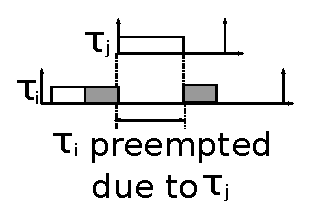
\includegraphics[scale=0.7]{figures/figure8}\caption{\label{fig8}Transactional retry due to release of higher priority
tasks}
\end{figure}

\end{proof}

\begin{clm}\label{rcm rlease conflict}
Under RCM and G-RMA/LCM, the total retry cost suffered by all transactions in any $\tau_i^x$ during an interval $L\le T_i$ is upper bounded by:
\begin{equation}
RC_{to}(L)=RC(L)+RC_{re}(L)
\label{total rc rcm eq}
\end{equation}
%
where $RC(L)$ and $RC_{re}(L)$ are defined in Claim~\ref{ecm rlease conflict}. $RC(L)$ is calculated by (16) in~\cite{stmconcurrencycontrol:emsoft11} for RCM, and (8) in~\cite{lcmdac2012} for G-RMA/LCM. $RC_{re}(L)$ is calculated by:
\begin{equation}
RC_{re}(L)=\sum_{\forall \tau_j \in \zeta_i^*}\left(\left\lceil\frac{L}{T_j}\right\rceil s_{i_{max}}\right)\label{eq21}
\end{equation}
%
where $\zeta_i^*=\{\tau_j:p_j > p_i \}$.
\end{clm}
\begin{proof}
The proof is the same as that for Claim~\ref{ecm rlease conflict}, except that G-RMA uses static priority. Thus, the carried-out jobs will be considered in the  interference with $\tau_i^x$. The carried-in jobs are still not considered because they are released before $r_i^x$. Claim follows.
\end{proof}
\begin{clm}\label{lock free release}
Consider lock-free synchronization. Let $r_{i_{max}}$ be the maximum execution cost of a single iteration of any retry loop of $\tau_i$. $RC_{re}$ under G-EDF  with lock-free synchronization is calculated by~(\ref{eq6}), where $s_{i_{max}}$ is replaced by $r_{i_{max}}$. $RC_{re}$ under G-RMA with lock-free synchronization is calculated by~(\ref{eq21}), where $s_{i_{max}}$ is replaced by $r_{i_{max}}$.
\end{clm}
%
\begin{proof}
The interference pattern of higher priority jobs to lower priority jobs is the same in ECM, G-EDF/LCM and G-EDF with lock-free synchronization. The pattern is also the same in RCM, G-RMA/LCM and G-RMA with lock-free. Claim follows.
\end{proof}


\subsection{PNF versus ECM\label{pnf vs ecm sec}}

\begin{clm}\label{PNF ecf comaprison clm}
The schedulability of PNF with G-EDF is better or equal to the schedulability  of ECM when conflicting atomic sections have equal lengths.
\end{clm}
\begin{proof}
Substitue $RC_{A}(T_{i})$ and $RC_{B}(T_{i})$ in (\ref{utilization comparison})
with (\ref{rc-PNF}) and (\ref{total rc ecm eq}), respectively. Let $\theta_{i}^{ex}=\theta_{i}+\theta_{i}^{*}$, where $\theta_{i}^{*}$
is the set of objects not accessed directly by $\tau_{i}$ but can
cause transactions in $\tau_{i}$ to retry due to transitive retry.
Let $\gamma_{i}^{ex}=\gamma_{i}+\gamma_{i}^{*}$, where $\gamma_{i}^{*}$
is the set of tasks that access objects in $\theta_{i}^{*}$.

Let:
%
\begin{comment}
\begin{eqnarray*}
g(\tau_{i}) & = & \left(\sum_{\forall\tau_{j}\in\gamma_{i}^{*}}\sum_{\theta\in\theta_{i}^{*}}\left(\left\lceil \frac{T_{i}}{T_{j}}\right\rceil \sum_{\forall\bar{s_{j}^{k}(\theta)}}len\left(\bar{s_{j}^{k}(\theta)}\\
& + & s_{max}^{*}(\theta)\right)\right)\right) + RC_{re}(T_{i})
\end{eqnarray*}
\end{comment}
\begin{eqnarray*}
g(\tau_{i}) & = & \Bigg(\sum_{\forall\tau_{j}\in\gamma_{i}^{*}}\sum_{\theta\in\theta_{i}^{*}}\Bigg(\left\lceil \frac{T_{i}}{T_{j}}\right\rceil \sum_{\forall\bar{s_{j}^{k}(\theta)}}len\Big(\bar{s_{j}^{k}(\theta)}\\
 & + & s_{max}^{*}(\theta)\Big)\Bigg)\Bigg)+RC_{re}(T_{i})
\end{eqnarray*}
%
where $RC_{re}$ is given by~(\ref{eq6}). Let:
%
\begin{equation*}
\eta_{1}(\tau_{i})=\sum_{\forall\tau_{j}\in\gamma_{i}}\sum_{\forall\theta\in\theta_{i}}\left(\sum_{\bar{\forall s_{j}^{k}(\theta)}}len\left(\bar{s_{j}^{k}(\theta)}\right)\right)
\end{equation*}
%
\begin{equation*}
\eta_{2}(\tau_{i})=\sum_{\forall\tau_{j}\in\gamma_{i}}\sum_{\forall\theta\in\theta_{i}}\left(\left\lceil \frac{T_{i}}{T_{j}}\right\rceil \sum_{\forall\bar{s_{j}^{k}(\theta)}}len\left(s_{max}^{j}(\theta)\right)\right)
\end{equation*}
%
and
%
\begin{equation*}
\eta_{3}(\tau_{i})=\sum_{\forall\tau_{j}\in\gamma_{i}}\sum_{\forall\theta\in\theta_{i}}\left(\left\lceil \frac{T_{i}}{T_{j}}\right\rceil \sum_{\bar{\forall s_{j}^{k}(\theta)}}len\left(\bar{s_{j}^{k}(\theta)}\right)\right)
\end{equation*}
%
By substitution of $g(\tau_{i})$, $\eta_1(\tau_i)$, and $\eta_2(\tau_i)$, and subtraction of $\sum_{\forall \tau_i} \frac{\eta_3(\tau_i)}{T_i}$ from both sides of (\ref{utilization comparison}), we get: 
\begin{equation}
\sum_{\forall \tau_i} \frac{\eta_1(\tau_i)}{T_i} \le \sum_{\forall \tau_i} \frac{\eta_2(\tau_i)+g(\tau_i)}{T_i}
\label{PNF ecm comparison 2}
\end{equation}
From (\ref{PNF ecm comparison 2}), we note that by keeping
every $len(\bar{s_{j}^{k}(\theta)})\le len(s_{max}^{j}(\theta))$
for each $\tau_{i}$, $\tau_{j}\in\gamma_{i}$, and $\theta\in\theta_{i}$,  (\ref{PNF ecm comparison 2}) holds. 
%
Because of the dynamic priority of G-EDF, $s_{max}^{j}(\theta)$
can belong to any task other than $\tau_{j}$. Assume four jobs $\tau_a^b$, $\tau_c^d$, $\tau_e^f$, and $\tau_g^h$ with a common object $\theta$. Let $s_{max}(\theta)=s_{g_{max}}(\theta)$. When $\tau_a^b$ is the checked $\tau_i$ by~(\ref{PNF ecm comparison 2}), any $s_c^x(\theta)$ and $s_e^y(\theta)$ will be less or equal to $s_{g_{max}}(\theta)$. But $s_{e_{max}}(\theta)$ should also be smaller or equal to either $s_{a_{max}}(\theta)$ or $s_{c_{max}}(\theta)$ or $s_{g_{max}}(\theta)$. Thus, there must be at least two equal maximum-length atomic sections in different tasks that access $\theta$. By generalizing the previous concept to every $\tau_i$, $\tau_j \in \gamma_i$,  and $\theta \in \theta_i$, claim follows.
\end{proof}

\subsection{PNF versus RCM}\label{pnf vs rcm sec}

\begin{clm}\label{clm_pnf_rcm_comp}
The schedulability of PNF with G-RMA is better or equal to the schedulability of RCM when a large number of tasks are heavily conflicting together. Increasing atomic section length of higher priority tasks improves schedulability of PNF compared with G-RMA/LCM schedulabiltiy.
\end{clm}
\begin{proof}
Let $\theta_{i}^{ex}=\theta_{i}+\theta_{i}^{*}$ and $\gamma_{i}^{ex}=\gamma_{i}+\gamma_{i}^{*}$, as defined in the proof of Claim~\ref{PNF ecf comaprison clm}. Substitute $RC_{A}(T_{i})$ and $RC_{B}(T_{i})$ in (\ref{utilization comparison}) with (\ref{rc-PNF}) and (\ref{total rc rcm eq}), respectively.
Let 
% 
\begin{eqnarray*}
g(\tau_{i}) & =RC_{re}(T_{i})+\Bigg( & \sum_{\forall\tau_{j}\in(\gamma_{i}^{*}\cap\zeta_{i}^{*})}\sum_{\forall\theta\in\theta_{i}^{*}}\left(\left\lceil \frac{T_{i}}{T_{j}}\right\rceil +1\right)\times\\
 &  & \sum_{\forall\bar{s_{j}^{k}(\theta)}}len\left(\bar{s_{j}^{k}(\theta)}+s_{max}^{j}(\theta)\right)\Bigg)
\end{eqnarray*}
%
where $RC_{re}$ and $\zeta_i^*$ are defined by~(\ref{eq21}).
Let $\gamma_{i}=\zeta_{i}^{*}\cup\bar{\zeta_{i}}$, where $\bar{\zeta_{i}}=\left\{ \tau_{j}:\left(\tau_{j}\ne\tau_{i}\right)\wedge\left(p_{j}<p_{i}\right)\right\} $,
thus $\zeta_{i}^{*}\cap\bar{\zeta_{i}}=\phi$.

Let:
%
\begin{equation*}
\eta_{1}(\tau_{i})=\sum_{\forall\tau_{j}\in(\gamma_{i}\cap\zeta_{i}^{*})}\sum_{\forall\theta\in\theta_{i}}\left(\left(\left\lceil \frac{T_{i}}{T_{j}}\right\rceil +1\right)\sum_{\bar{\forall s_{j}^{k}(\theta)}}len\left(\bar{s_{j}^{k}(\theta)}\right)\right)
\end{equation*}
%
\begin{equation*}
\eta_{2}(\tau_{i})=\sum_{\forall\tau_{j}\in(\gamma_{i}\cap\bar{\zeta_{i}})}\sum_{\forall\theta\in\theta_{i}}\left(\left(\left\lceil \frac{T_{i}}{T_{j}}\right\rceil +1\right)\sum_{\bar{\forall s_{j}^{k}(\theta)}}len\left(\bar{s_{j}^{k}(\theta)}\right)\right)
\end{equation*}
%
and
%
\begin{eqnarray*}
\eta_{3}(\tau_{i}) & = & \sum_{\forall\tau_{j}\in(\gamma_{i}\cap\zeta_{i}^{*})}\sum_{\forall\theta\in\theta_{i}}\Bigg(\left(\left\lceil \frac{T_{i}}{T_{j}}\right\rceil +1\right)\times\\
 &  & \sum_{\forall\bar{s_{j}^{k}(\theta)}}len\left(\bar{s_{j}^{k}(\theta)}+s_{max}^{j}(\theta)\right)\Bigg)
\end{eqnarray*}
%
By substitution of $g(\tau_i)$, $\eta_1(\tau_i)$, $\eta_2(\tau_i)$, and $\eta_3(\tau_i)$ in (\ref{utilization comparison}), we get:
%
\begin{equation}
\sum_{\forall\tau_{i}}\frac{\eta_{1}(\tau_{i})+\eta_{2}(\tau_{i})}{T_{i}}\le\sum_{\forall\tau_{i}}\frac{\eta_{3}(\tau_{i})+g(\tau_{i})}{T_{i}}
\label{PNF rcm comparison 3}
\end{equation}
%
When tasks with deadlines equal to periods are scheduled with G-RMA, $T_{j}>T_{i}$ if $p_{j}<p_{i}$. So, for each $\tau_{j}\in\bar{\zeta_{i}}$, $\left\lceil \frac{T_{i}}{T_{j}}\right\rceil =1$. Then:
%
\begin{equation}
\eta_{2}(\tau_{i})=2\sum_{\forall\tau_{j}\in(\gamma_{i}\cap\bar{\zeta_{i}})}\sum_{\forall\theta\in\theta_{i}}\sum_{\bar{\forall s_{j}^{k}(\theta)}}len\left(\bar{s_{j}^{k}(\theta)}\right)
\label{PNF rcm comparison 5}
\end{equation}
%
Let:
%
\begin{equation*}
\eta_{4}(\tau_{i})=\sum_{\forall\tau_{j}\in(\gamma_{i}\cap\zeta_{i}^{*})}\sum_{\forall\theta\in\theta_{i}}\left(\left\lceil \frac{T_{i}}{T_{j}}\right\rceil +1\right)\sum_{\forall\bar{s_{j}^{k}(\theta)}}len\left(s_{max}^{j}(\theta)\right)
\end{equation*}
%
By substitution of~(\ref{PNF rcm comparison 5}) and subtraction of $\sum_{\forall \tau_i} \frac{\eta_1 (\tau_i)}{T_i}$ from both sides of~(\ref{PNF rcm comparison 3}), we get:
%
\begin{equation}
2\sum_{\forall\tau_{i}}\frac{\eta_{2}(\tau_{i})}{T_{i}}\le\sum_{\forall\tau_{i}}\frac{\eta_{4}(\tau_{i})+g(\tau_{i})}{T_{i}}
\label{PNF rcm comparison 4}
\end{equation}
%
From (\ref{PNF rcm comparison 4}), we note that when higher priority jobs increasingly conflict with lower priority jobs, 
(\ref{PNF rcm comparison 4}) tends to hold. This occurs when the number of conflicting tasks, their job instances, and their shared objects increases. 
When the number of shared objects among tasks increases, $g(\tau_{i})$ also increases. This allows (\ref{PNF rcm comparison 4}) to
hold. Claim follows.
\end{proof}

%SH-ST
\subsection{PNF versus G-EDF/LCM}

\begin{clm}\label{sub:pnf_lcm_edf_comp}

Schedulability of PNF/EDF is equal or better than schedulability of G-EDF/LCM if lengths of conflicting atomic sections are approximately equal and all $\alpha$s approach unity.

\end{clm}

\begin{proof}

Assuming $\eta_{1}(\tau_i)$ and $\eta_{3}(\tau_i)$ are the same as defined in proof
of Claim~\ref{PNF ecf comaprison clm}. Let 

\begin{eqnarray*}
g(\tau_{i}) & = & \Bigg(\sum_{\forall\tau_{j}\in\gamma_{i}^{*}}\sum_{\theta\in\theta_{i}^{*}}\Bigg(\left\lceil \frac{T_{i}}{T_{j}}\right\rceil \sum_{\forall\bar{s_{j}^{k}(\theta)}}len\Big(\bar{s_{j}^{k}(\theta)}\\
 & + & \alpha_{max}^{ji}s_{max}^{*}(\theta)\Big)\Bigg)\Bigg)+RC_{re}(T_{i})
\end{eqnarray*}


\[
\eta_{2}(\tau_{i})=\sum_{\forall\tau_{j}\in\gamma_{i}}\sum_{\forall\theta\in\theta_{i}}\left(\left\lceil \frac{T_{i}}{T_{j}}\right\rceil \sum_{\forall\bar{s_{j}^{k}(\theta)}}len\left(\alpha_{max}^{jl}s_{max}^{j}(\theta)\right)\right)
\]
Following the same steps in proof of Claim~\ref{PNF ecf comaprison clm}, we get 
\begin{equation}
\sum_{\forall\tau_{i}}\frac{\eta_{1}(\tau_{i})}{T_{i}}\le\sum_{\forall\tau_{i}}\frac{\eta_{2}(\tau_{i})+g(\tau_{i})}{T_{i}}\label{eq:pnf_lcm_edf_comp}
\end{equation}
Assuming $g(\tau_{i})_{\forall\tau_{i}}\rightarrow0$, thus neglecting
the effect of transitive retry and retry cost due to release of higher
priority jobs. Let $len(\bar{s_{j}^{k}(\theta)})=s_{max}^{j}(\theta)=s$,
and $\alpha_{max}^{jl}=\alpha_{max}^{iy}=1$ in (\ref{eq:pnf_lcm_edf_comp}),
then schedulability of PNF/EDF equals schedulability of LCM/EDF if
$\left\lceil \frac{T_{i}}{T_{j}}\right\rceil =1,\,\forall\tau_{i},\tau_{j}$
(which means equal periods for all tasks). If $\left\lceil \frac{T_{i}}{T_{j}}\right\rceil >1,\,\forall\tau_{i},\tau_{j}$,
then schedulability of PNF/EDF is better than LCM/EDF. Schedulability
of PNF/EDF becomes more better than schedulability of LCM/EDF if $g(\tau_{i})$
is not zero. Claim follows.
\end{proof}

\subsection{PNF versus G-RMA/LCM}

\begin{clm}\label{sub:pnf_lcm_rma_comp}

Schedulability performance of PNF is equal or better than schedulability performance of G-RMA/LCM if: 1) conflict effect of higher priority tasks to lower priority tasks increases. 2)Lengths of atomic sections increase as tasks' priorities increase. 3) $\alpha$s approach unity.

\end{clm}

\begin{proof}

Assume $g(\tau_{i})$, $\eta_{1}(\tau_{i})$, $\eta_{2}(\tau_{i})$ are the same as proof of Claim~\ref{clm_pnf_rcm_comp}. Let 
\begin{eqnarray*}
\eta_{3}(\tau_{i}) & = & \sum_{\forall\tau_{j}\in(\gamma_{i}\cap\zeta_{i}^{*})}\sum_{\forall\theta\in\theta_{i}}\Bigg(\left(\left\lceil \frac{T_{i}}{T_{j}}\right\rceil +1\right)\times\\
 &  & \sum_{\forall\bar{s_{j}^{k}(\theta)}}len\left(\bar{s_{j}^{k}(\theta)}+\alpha_{max}^{jl}s_{max}^{j}(\theta)\right)\Bigg)
\end{eqnarray*}
Following the setps of proof of Claim~\ref{clm_pnf_rcm_comp}

\begin{equation}
\therefore\sum_{\forall\tau_{i}}\frac{\eta_{1}(\tau_{i})+\eta_{2}(\tau_{i})}{T_{i}}\le\sum_{\forall\tau_{i}}\frac{\eta_{3}(\tau_{i})+g(\tau_{i})}{T_{i}}\label{pnf-lcm-rma-comp-1}
\end{equation}
Let 
\begin{eqnarray*}
\eta_{4}(\tau_{i}) & = & \sum_{\forall\tau_{j}\in(\gamma_{i}\cap\zeta_{i}^{*})}\sum_{\forall\theta\in\theta_{i}}\Bigg(\left(\left\lceil \frac{T_{i}}{T_{j}}\right\rceil +1\right)\\
 & \times & \sum_{\forall\bar{s_{j}^{k}(\theta)}}len\left(\alpha_{max}^{jl}s_{max}^{j}(\theta)\right)\Bigg)
\end{eqnarray*}
$\therefore$(\ref{pnf-lcm-rma-comp-1}) becomes

\begin{equation}
2\sum_{\forall\tau_{i}}\frac{\eta_{2}(\tau_{i})}{T_{i}}\le\sum_{\forall\tau_{i}}\frac{\eta_{4}(\tau_{i})+g(\tau_{i})}{T_{i}}\label{pnf-lcm-rma-comp-2}
\end{equation}
Assuming negligible effect of transitive retry and retry cost due
to release of higher priority jobs ($g(\tau_{i})\rightarrow0$). (\ref{pnf-lcm-rma-comp-2})
holds if: 1) contention from higher priority jobs to lower priority
jobs increases because of the $\left\lceil \frac{T_{i}}{T_{j}}\right\rceil +1$
term in the right hand side of (\ref{pnf-lcm-rma-comp-2}). 2) $\alpha$s
approaches unity. 3) Lengths of atomic sections increase as priority
increases. This makes $len(s_{max}^{j}(\theta))$ in the right hand
side of (\ref{pnf-lcm-rma-comp-2}) greater than $len(\bar{s_{j}^{k}(\theta)})$.
Claim follows.

\end{proof}

\subsection{PNF versus lock-free\label{pnf vs lock free sec}}

Lock-free synchronization~\cite{key-5,stmconcurrencycontrol:emsoft11} accesses only one object. Thus, the number of accessed objects per transaction in PNF is limited to one. This allows us to compare the schedulability of PNF with the lock-free algorithm. 

$RC_{B}(T_{i})$ in (\ref{utilization comparison}) is replaced with:
%
\begin{equation}
\sum_{\forall\tau_{j}\in\gamma_{i}}\Bigg(\left(\left\lceil \frac{T_{i}}{T_{j}}\right\rceil +1\right)\beta_{i,j}r_{max}\Bigg)+RC_{re}(T_{i})
\label{lock-free rc}
\end{equation}
%
where $\beta_{i,j}$ is the number of retry loops of $\tau_{j}$ that access the same object as accessed by some retry loop of $\tau_{i}$~\cite{key-5}. $r_{max}$ is the maximum execution cost of a single iteration of any retry loop of any task~\cite{key-5}. $RC_{re}(T_i)$ is defined in Claim~\ref{lock free release}. Lock-free synchronization does not depend on priorities  of tasks. Thus,~(\ref{lock-free rc}) applies for both G-EDF and G-RMA systems.


%%
\begin{clm}\label{PNF lock-free comparison}
Let $r_{max}$ be the maximum execution cost of a single iteration of any retry loop of any task~\cite{key-5}. Let $s_{max}$ be the maximum transaction length in all tasks. Assume that each transaction under PNF accesses only one object for once. The schedulability of PNF with either G-EDF or G-RMA scheduler is better or equal to the schedulability of lock-free
synchronization if $s_{max}/r_{max}\le 1$.
\end{clm}
\begin{proof}
The assumption in Claim~\ref{PNF lock-free comparison} is made to enable a comparison between PNF and the lock-free technique. Let $RC_{A}(T_{i})$ in (\ref{utilization comparison}) be replaced
with (\ref{rc-PNF}) and $RC_{B}(T_{i})$ be replaced with (\ref{lock-free rc}).
To simplify comparison, (\ref{rc-PNF}) is upper bounded by:
%
\begin{equation*}
RC(T_{i})=\sum_{\tau_{j}\in\gamma_{i}}\left(\left(\left\lceil \frac{T_{i}}{T_{j}}\right\rceil +1\right)\beta_{i,j}^* s_{max}\right)
\end{equation*}
%
where $\beta_{i,j}^*$ is the number of times transactions in $\tau_j$ accesses shared objects with $
\tau_i$. Thus, $\beta_{i,j}^* = \beta_{i,j}$. Thus, (\ref{utilization comparison}) will be:
\begin{eqnarray}
\sum_{\forall\tau_{i}}\frac{\sum_{\tau_{j}\in\gamma_{i}}\left(\left(\left\lceil \frac{T_{i}}{T_{j}}\right\rceil +1\right)\beta_{i,j}s_{max}\right)}{T_{i}} & \le\nonumber \\
\sum_{\forall\tau_{i}}\frac{\sum_{\forall\tau_{j}\in\gamma_{i}}\left(\left\lceil \frac{T_{i}}{T_{j}}\right\rceil +1\right)\beta_{i,j}r_{max}+RC_{re}(\tau_i)}{T_{i}}\label{PNF lock-free comparison}
\end{eqnarray}
From (\ref{PNF lock-free comparison}), we note that if $s_{max}\le r_{max}$,
then (\ref{PNF lock-free comparison}) holds. Claim follows.
\end{proof}

\section{Conclusions}

Transitive retry increases transactions' retry cost under ECM, RCM and LCM. PNF is designed to avoid transitive retry by non preempting transaction at execution. Aborted transactions are ordered in priority in $n\_set$ list. When an executing transaction commits, it triggers the highest priority transaction $s_i^j$ in the $n\_set$ to check conflicts with executing transactions. $s_i^j$, in turn, triggers the second transaction in the $n\_set$, and so on. Priority of aborted transactions is reduced to enable other tasks to execute. Thus, increasing processor usage. Executing transactions are not preempted due to release of higher priority jobs. In case of the other CMs, retry due to release of higher priority jobs depends on the CM implementation. On the negative side of PNF, higher priority jobs can be blocked by executing transactions belonging to lower priority jobs. Thus, increasing their response time. Schedulability under EDF/PNF is equal or better to ECM schedulability when lengths of atomic sections are are almost equal. RMA/PNF schedulability is equal or better than RCM in case of high conflict from higher priority jobs to lower priority ones. The previous conditions apply to schedulability comparison between PNF and LCM, in addition to increasing $\alpha$s to unity. This is logical as LCM with G-EDF(G-RMA) acts as ECM(RCM) with $\alpha\rightarrow 1$. For schedulability of PNF to be equal or better than lock-free, the upper bound on $s_{max}/r_{max}$ is 1 instead of 0.5 under ECM and RCM. In the future, we are looking for combining PNF and LCM. This combination enables CM to act as PNF in case of highly transitive retry, and act as LCM otherwise. Thus, retry cost is reduced in all cases.


%%%%%%%%%%%%%%%%%%%%%%%%%%%%%%%%

\chapter{\label{ch_exp}Experiments}
\markright{Mohammed Elshambakey \hfill Chapter 6. Experiments \hfill}

\section{LCM, ECM and RCM}
Having established LCM's retry and response time upper bounds, and the conditions under which it outperforms ECM, RCM, and lock-free synchronization, we now would like to understand how LCM's retry and response times in practice (i.e., on average) compare with that of competitor methods. Since this can only be understood experimentally, we implement LCM and the competitor methods and conduct experimental studies. 

\subsection{Experimental Setup}
We used the ChronOS real-time Linux kernel~\cite{dellinger2011chronos}
and the RSTM library~\cite{marathe2006lowering}. We modified RSTM to include implementations of ECM, RCM, G-EDF/LCM, and G-RMA/LCM contention managers, and modified ChronOS to include implementations of G-EDF and G-RMA schedulers. 

For the retry-loop lock-free implementation,
we used a loop that reads an object and attempts to write to the object using a compare-and-swap (CAS) instruction. The task retries until the CAS succeeds. 
%We call this lock-free operation, CAS-loop operation.

We use an 8 core, 2GHz AMD Opteron platform. The average time
taken for one write operation by RSTM on any
core is 0.0129653375$\mu s$, and the average time taken
by one CAS-loop operation on any core is 0.0292546250 $\mu s$.

We used the periodic task set shown in Table~\ref{tab:Task-set-1}. Each task runs in its own thread and has a set of atomic sections. Atomic section properties are probabilistically controlled (for experimental evaluation) using three parameters: the maximum and minimum lengths of any atomic section within the task, and the total length of atomic sections within any task. All task atomic sections access the same object, and do write operations on the object (thus, contention is the highest).

\begin{table}
\caption{\label{tab:Task-set-1}Task sets. (a) \label{tab:Task-sets-(a)} Task set 1: 5-task set; 
\label{tab:Task-sets-(b)} (b) Task set 2: 10-task set; \label{tab:Task-sets-(c)} (c) Task set 3: 12-task set}
\centering{}\begin{tabular}{|c|c|c|}
\multicolumn{3}{c}{(a)}\tabularnewline
\cline{2-3} 
\multicolumn{1}{c|}{} & $T_{i}(\mu s)$ & $c_{i}(\mu s)$\tabularnewline
\hline 
$\tau_{1}$ & 500000 & 150000\tabularnewline
\hline 
$\tau_{2}$ & 1000000 & 227000\tabularnewline
\hline 
$\tau_{3}$ & 1500000 & 410000\tabularnewline
\hline 
$\tau_{4}$ & 3000000 & 299000\tabularnewline
\hline 
$\tau_{5}$ & 5000000 & 500000\tabularnewline
\hline
\end{tabular} \begin{tabular}{|c|c|c|}
\multicolumn{3}{c}{(b)}\tabularnewline
\cline{2-3} 
\multicolumn{1}{c|}{} & $T_{i}(\mu s)$ & $c_{i}(\mu s)$\tabularnewline
\hline 
$\tau_{1}$ & 400000 & 75241\tabularnewline
\hline 
$\tau_{2}$ & 750000 & 69762\tabularnewline
\hline 
$\tau_{3}$ & 1200000 & 267122\tabularnewline
\hline 
$\tau_{4}$ & 1500000 & 69863\tabularnewline
\hline 
$\tau_{5}$ & 2400000 & 152014\tabularnewline
\hline 
$\tau_{6}$ & 4000000 & 286301\tabularnewline
\hline 
$\tau_{7}$ & 7500000 & 493150\tabularnewline
\hline 
$\tau_{8}$ & 10000000 & 794520\tabularnewline
\hline 
$\tau_{9}$ & 15000000 & 1212328\tabularnewline
\hline 
$\tau_{10}$ & 20000000 & 1775342\tabularnewline
\hline
\end{tabular} \begin{tabular}{|c|c|c|}
\multicolumn{3}{c}{(c)}\tabularnewline
\cline{2-3} 
\multicolumn{1}{c|}{} & $T_{i}(\mu s)$ & $c_{i}(\mu s)$\tabularnewline
\hline 
$\tau_{1}$ & 400000 & 58195\tabularnewline
\hline 
$\tau_{2}$ & 750000 & 53963\tabularnewline
\hline 
$\tau_{3}$ & 1000000 & 206330\tabularnewline
\hline 
$\tau_{4}$ & 1200000 & 53968\tabularnewline
\hline 
$\tau_{5}$ & 1500000 & 117449\tabularnewline
\hline 
$\tau_{6}$ & 2400000 & 221143\tabularnewline
\hline 
$\tau_{7}$ & 3000000 & 290428\tabularnewline
\hline 
$\tau_{8}$ & 4000000 & 83420\tabularnewline
\hline 
$\tau_{9}$ & 7500000 & 380917\tabularnewline
\hline 
$\tau_{10}$ & 10000000 & 613700\tabularnewline
\hline 
$\tau_{11}$ & 15000000 & 936422\tabularnewline
\hline 
$\tau_{12}$ & 20000000 & 1371302\tabularnewline
\hline
\end{tabular}
\end{table}

\subsection{Results}

Figure \ref{fig:RC_results} shows the retry cost (RC) 
for each task in the three task sets in Table \ref{tab:Task-set-1}, where each task has a single atomic section of length equal to 0.2 of the task length. Each data point in the figure has a confidence level of 0.95. We observe that G-EDF/LCM and G-RMA/LCM achieve shorter
or comparable retry cost than ECM and RCM. Since all tasks are initially
released at the same time, and due to the specific nature of task properties, tasks with lower IDs somehow have higher priorities under the G-EDF scheduler. Note that tasks with lower IDs have higher priorities under G-RMA, since tasks are ordered in non-decreasing order of their periods. 

Thus, we observe that G-EDF/LCM and G-RMA/LCM achieve comparable retry costs
to ECM and RCM for some tasks with lower IDs. But when task ID increases,
LCM --- for both schedulers --- achieves much shorter retry costs 
than ECM and RCM. 
This is because, higher priority tasks in LCM can be delayed by lower priority tasks, which is not the case for ECM and RCM. However, as task priority decreases, LCM, by definition, prevents higher priority
tasks from aborting lower priority ones if a higher priority task
interferes with a lower priority one after a specified threshold. In contrast, under ECM and RCM, lower priority tasks abort in favor of higher priority ones. G-EDF/LCM and G-RMA/LCM also achieve shorter retry costs than the retry-loop lock-free algorithm.

\begin{figure}[htbp]
\centering
\subfigure[Task set 1]{
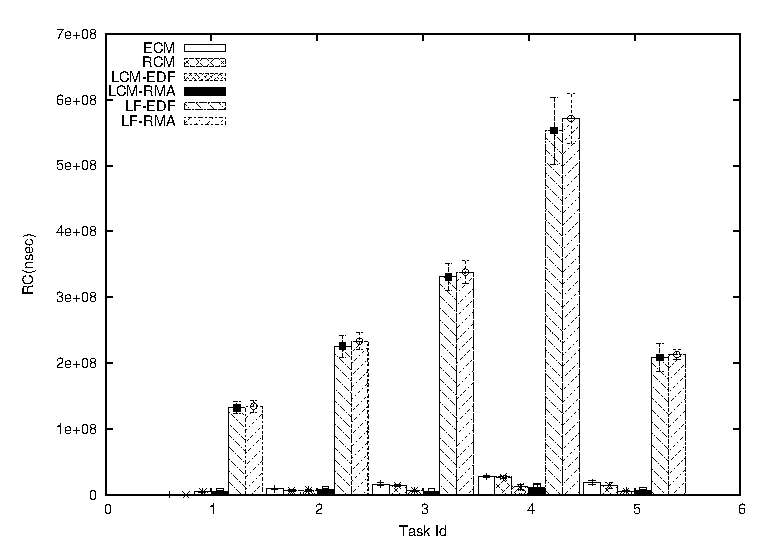
\includegraphics[scale=0.6]
{figures/Abr_dur_5t_nl_g_30_0.2_0.2_0.2_1.eps}
\label{fig-RC-set1}
}
\subfigure[Task set 2]{
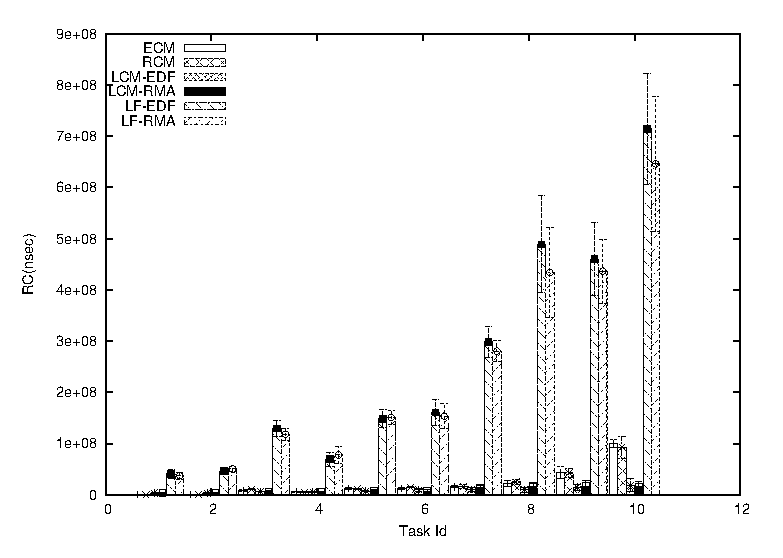
\includegraphics[scale=0.6]{figures/Abr_dur_10t_nl_g_30_0.2_0.2_0.2_1.eps}
\label{fig-RC-set2-1}
}
\subfigure[Task set 3]{
\includegraphics[scale=0.6]{figures/Abr_dur_12t_nl_g_30_0.2_0.2_0.2_1.eps}
\label{fig-RC-set3-1}
}
\caption{Task retry costs under LCM and competitor synchronization methods}
\label{fig:RC_results}
\end{figure}

Figure \ref{fig:res_results-1} shows the response time of each task of the task sets in Table \ref{tab:Task-set-1} with a confidence level of 0.95. (Again, each task's atomic section length is equal to half of the task length.) 
We observe that G-EDF/LCM and G-RMA/LCM achieve shorter 
response time than the retry-loop lock-free
algorithm, and shorter 
or comparable response time than ECM and RCM.

\begin{figure}[htbp]
\subfigure[Task set 1]{
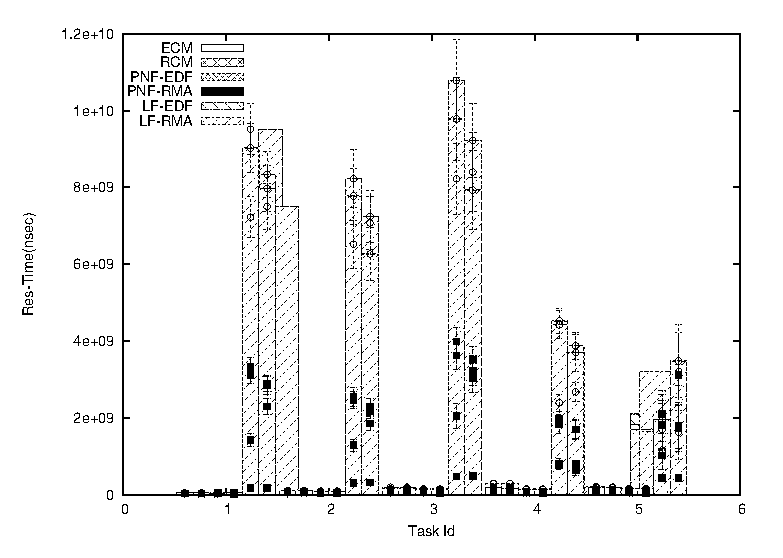
\includegraphics[scale=0.6]{figures/Res_Time_5t_nl_g_30_0.2_0.2_0.2_1.eps}
\label{fig-res-set1-1}
}
\subfigure[Task set 2]{
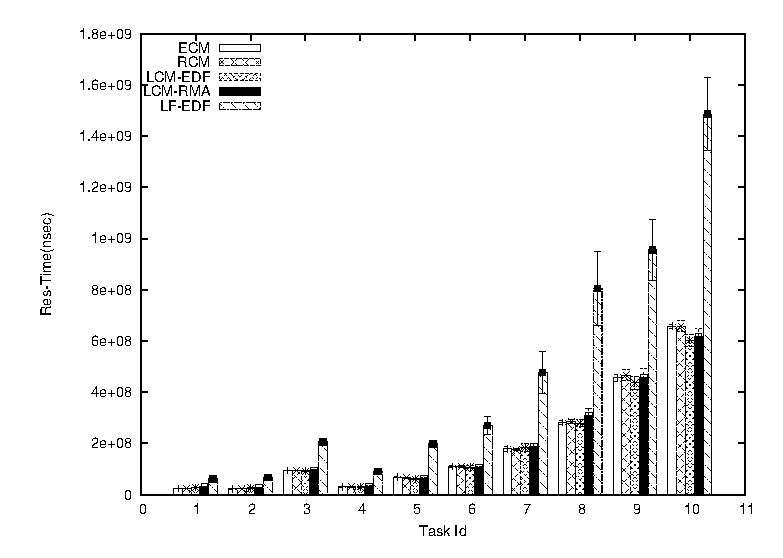
\includegraphics[scale=0.6]{figures/Res_Time_10t_nl_g_30_0.2_0.2_0.2_1.eps}
\label{fig-res-set2-1}
}
\subfigure[Task set 3 ]{
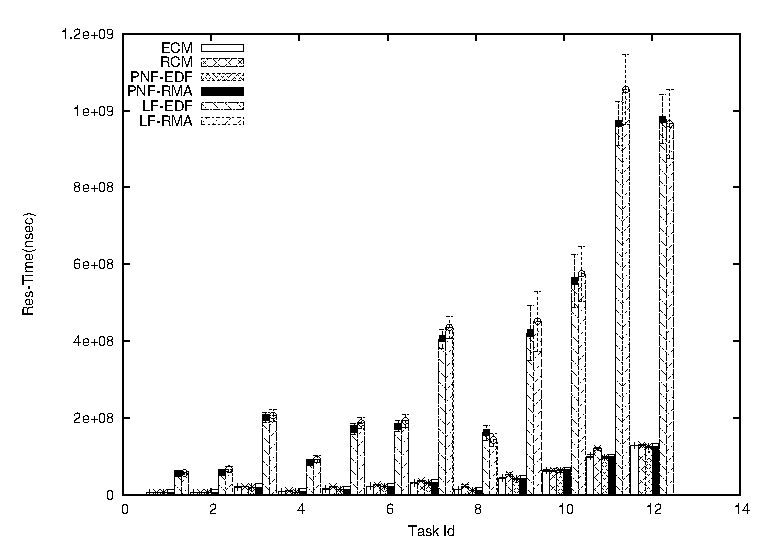
\includegraphics[scale=0.6]{figures/Res_Time_12t_nl_g_30_0.2_0.2_0.2_1.eps}
\label{fig-res-set3-1}
}
\caption{Task response times under LCM and competitor synchronization methods}
\label{fig:res_results-1}
\end{figure}

We repeated the experiments by varying the number and length of atomic sections. Due to space limitations, only a subset of the results are shown in Figures~\ref{fig:RC_results 5 2 2} to~\ref{fig:res_results 8 5 2}. 
(The complete set of results are shown in Appendix B of~\cite{stmconcurrencycontrol_techreport}.)
Each figure has three parameters $x$, $y$, and $z$ in the label. 
$x$ specifies the relative total length of all atomic sections to the length of the task. $y$ specifies the maximum relative length of any atomic section to the length of the task. $z$ specifies the minimum relative length of any atomic section to the length of the task. These figures show a consistent trend with previous results.

\begin{figure}[htbp]
\centering
\subfigure[Task set 1]{
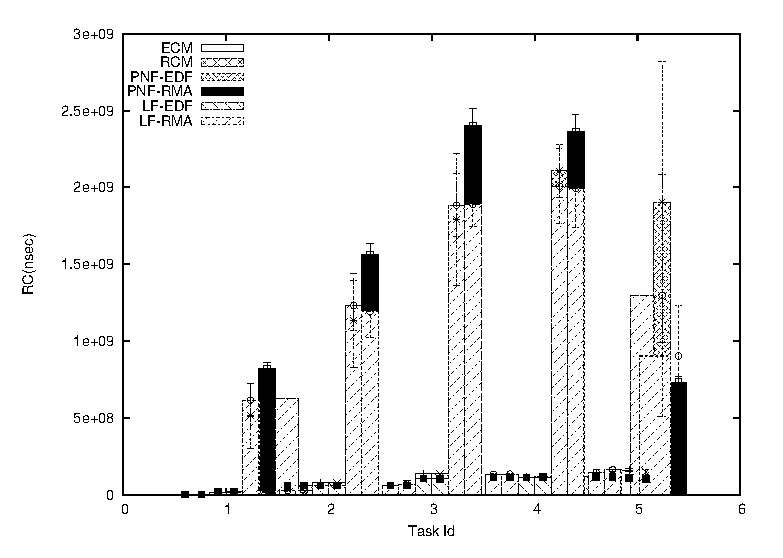
\includegraphics[scale=0.6]
{figures/Abr_dur_5t_nl_g_30_0.5_0.2_0.2_1.eps}
\label{fig-RC-set1}
}
\subfigure[Task set 2]{
\includegraphics[scale=0.6]{figures/Abr_dur_10t_nl_g_30_0.5_0.2_0.2_1.eps}
\label{fig-RC-set2-2}
}
\subfigure[Task set 3]{
\includegraphics[scale=0.6]{figures/Abr_dur_12t_nl_g_30_0.5_0.2_0.2_1.eps}
\label{fig-RC-set3-2}
}
\caption{Task retry costs under LCM and competitor synchronization methods (0.5,0.2,0.2)}
\label{fig:RC_results 5 2 2}
\end{figure}

\begin{figure}[htbp]
\subfigure[Task set 1]{
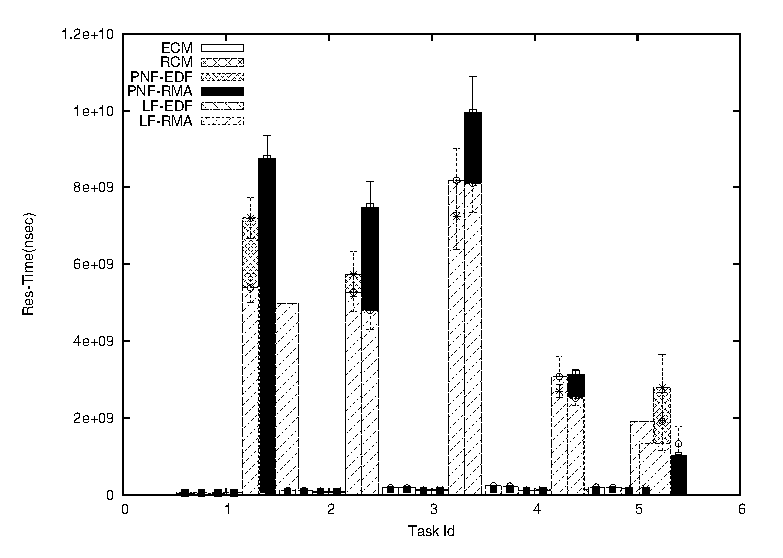
\includegraphics[scale=0.6]{figures/Res_Time_5t_nl_g_30_0.5_0.2_0.2_1.eps}
\label{fig-res-set1-1}
}
\subfigure[Task set 2]{
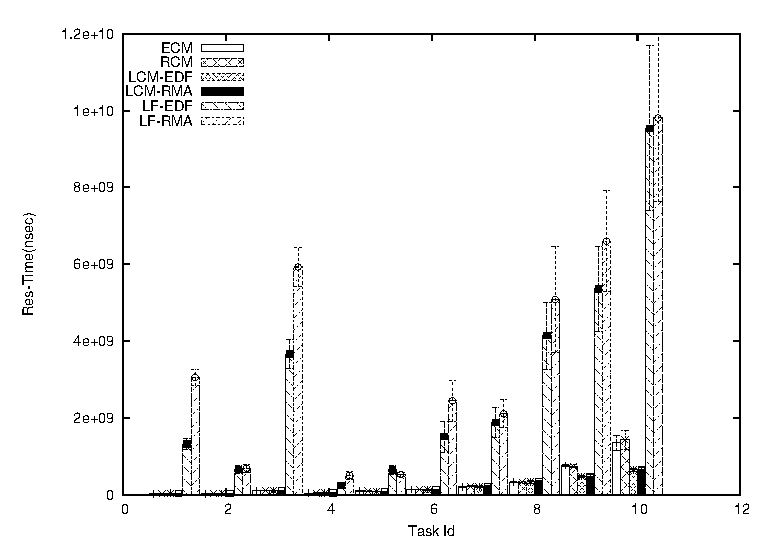
\includegraphics[scale=0.6]{figures/Res_Time_10t_nl_g_30_0.5_0.2_0.2_1.eps}
\label{fig-res-set2-1}
}
\subfigure[Task set 3 ]{
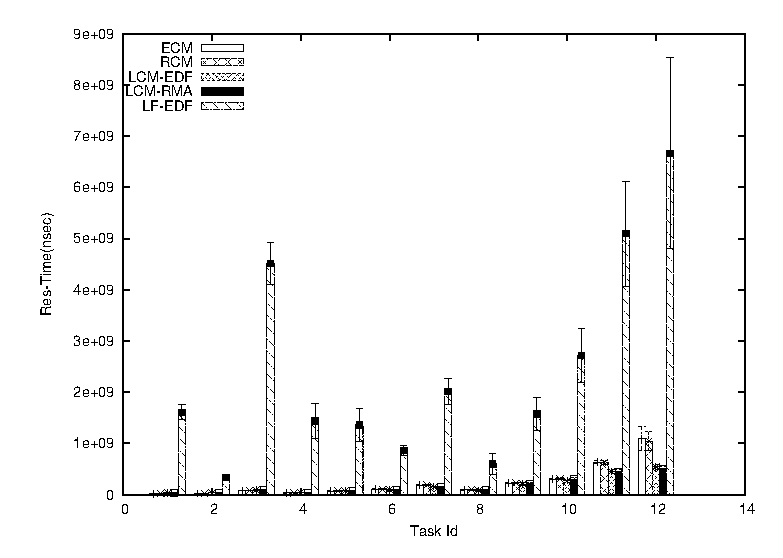
\includegraphics[scale=0.6]{figures/Res_Time_12t_nl_g_30_0.5_0.2_0.2_1.eps}
\label{fig-res-set3-1}
}
\caption{Task response times under LCM and competitor synchronization methods (0.5,0.2,0.2)}
\label{fig:res_results 5 2 2}
\end{figure}

\begin{figure}[htbp]
\centering
\subfigure[Task set 1]{
\includegraphics[scale=0.6]
{figures/Abr_dur_5t_nl_g_30_0.8_0.5_0.2_1.eps}
\label{fig-RC-set1}
}
\subfigure[Task set 2]{
\includegraphics[scale=0.6]{figures/Abr_dur_10t_nl_g_30_0.8_0.5_0.2_1.eps}
\label{fig-RC-set2-3}
}
\subfigure[Task set 3]{
\includegraphics[scale=0.6]{figures/Abr_dur_12t_nl_g_30_0.8_0.5_0.2_1.eps}
\label{fig-RC-set3-3}
}
\caption{Task retry costs under LCM and competitor synchronization methods (0.8,0.5,0.2)}
\label{fig:RC_results 8 5 2}
\end{figure}

\begin{figure}[htbp]
\subfigure[Task set 1]{
\includegraphics[scale=0.6]{figures/Res_Time_5t_nl_g_30_0.8_0.5_0.2_1.eps}
\label{fig-res-set1-1}
}
\subfigure[Task set 2]{
\includegraphics[scale=0.6]{figures/Res_Time_10t_nl_g_30_0.8_0.5_0.2_1.eps}
\label{fig-res-set2-1}
}
\subfigure[Task set 3 ]{
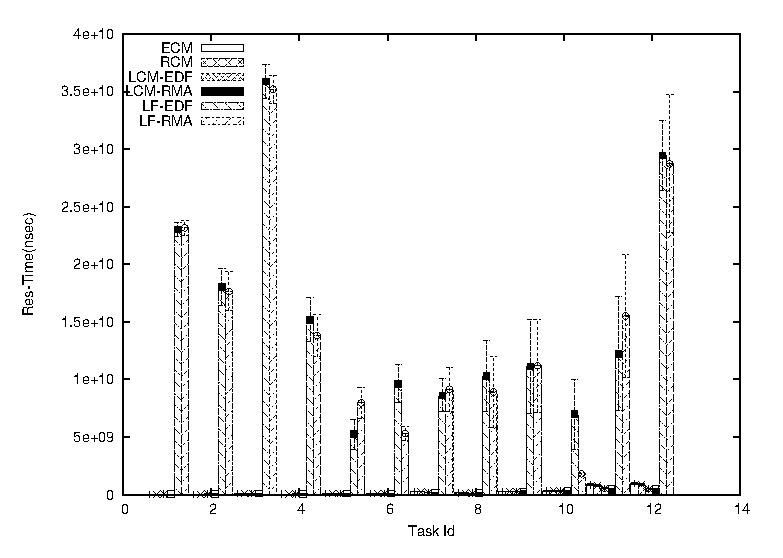
\includegraphics[scale=0.6]{figures/Res_Time_12t_nl_g_30_0.8_0.5_0.2_1.eps}
\label{fig-res-set3-1}
}
\caption{Task response times under LCM and competitor synchronization methods (0.8,0.5,0.2)}
\label{fig:res_results 8 5 2}
\end{figure}

\section{PNF}

Lock-free cannot handle more than object per atomic section. So, we compare retry cost of PNF against retry cost of other contention managers and lock-free in case of one object per transaction. Then, we compare retry cost of PNF against ECM, RCM and LCM in case of multiple objects per transactions. We used 3 sets of 4, 8 and 20 tasks. The structure of these tasks are shown in Table~\ref{pnf_task_sets_table}. The difficulty in testing with PNF is to incur transitive retry cases. Tasks are arranged in non-decreasing order of periods, and each task shares objects only with the previous and next tasks. Each task begins with an atomic section. Thus, increasing the opportunity of transitive retry.
\begin{flushleft}
\begin{table}[htbp]
\begin{centering}
\caption{\label{pnf_task_sets_table}Task sets \label{tab:Task-sets-a)pnf4}a) 4 tasks. \label{tab:Task-sets-a)pnf8}b)
8 tasks. \label{tab:Task-sets-a)pnf20}c) 20 tasks.}

\begin{tabular}{|c|c|}
\multicolumn{2}{c}{(a)}\tabularnewline
\hline 
$P_{i}(\mu s)$ & $c_{i}(\mu s)$\tabularnewline
\hline 
1000000 & 227000\tabularnewline
\hline 
1500000 & 410000\tabularnewline
\hline 
3000000 & 299000\tabularnewline
\hline 
5000000 & 500000\tabularnewline
\hline 
\end{tabular}~% 
\begin{tabular}{|c|c|}
\multicolumn{2}{c}{(b)}\tabularnewline
\hline 
$P_{i}(\mu s)$ & $c_{i}(\mu s)$\tabularnewline
\hline 
1500000 & 961000\tabularnewline
\hline 
1875000 & 175000\tabularnewline
\hline 
2500000 & 205000\tabularnewline
\hline 
3000000 & 129000\tabularnewline
\hline 
3750000 & 117000\tabularnewline
\hline 
5000000 & 269000\tabularnewline
\hline 
7500000 & 118000\tabularnewline
\hline 
15000000 & 609000\tabularnewline
\hline 
\end{tabular}~% 
\begin{tabular}{|c|c|}
\multicolumn{2}{c}{(c)}\tabularnewline
\hline 
$P_{i}(\mu s)$ & $c_{i}(\mu s)$\tabularnewline
\hline 
375000 & 9000\tabularnewline
\hline 
400000 & 8000\tabularnewline
\hline 
500000 & 8000\tabularnewline
\hline 
600000 & 14000\tabularnewline
\hline 
625000 & 375000\tabularnewline
\hline 
750000 & 19000\tabularnewline
\hline 
1000000 & 26000\tabularnewline
\hline 
1200000 & 17000\tabularnewline
\hline 
1250000 & 21000\tabularnewline
\hline 
1500000 & 33000\tabularnewline
\hline 
1875000 & 39000\tabularnewline
\hline 
2000000 & 43000\tabularnewline
\hline 
2500000 & 18000\tabularnewline
\hline 
3000000 & 90000\tabularnewline
\hline 
3750000 & 28000\tabularnewline
\hline 
5000000 & 126000\tabularnewline
\hline 
7500000 & 231000\tabularnewline
\hline 
10000000 & 407000\tabularnewline
\hline 
15000000 & 261000\tabularnewline
\hline 
30000000 & 369000\tabularnewline
\hline 
375000 & 8000\tabularnewline
\hline 
30000000 & 407000\tabularnewline
\hline 
\end{tabular}
\par\end{centering}

\end{table}

\par\end{flushleft}

Figure~\ref{fig:pnf_results_1_obj_all} shows average retry cost under ECM, RCM, LCM, PNF and lock-free. Figure~\ref{fig:pnf_results_1_obj_without_lock_free} shows average retry cost for only contention managers. Only one object per transaction is shared in Figures~\ref{fig:pnf_results_1_obj_all} and~\ref{fig:pnf_results_1_obj_without_lock_free}. Lock-free is still the longest technique as it provides no conflict resolution. LCM (with both G-EDF and G-RMA) is better than the others. PNF (with G-EDF and G-RMA) approximates ECM and RCM because there is no transitive retry here.

Figure~\ref{fig:pnf_results_multiobject} shows average retry cost for three task sets in case of multiple objects per transaction. Each data point in the figure has a confidence level of 0.95. PNF (with G-EDF and G-RMA) achieves shorter or comparable retry cost than ECM, RCM and LCM. In Figure~\ref{fig-RC-pnf-20t}, retry costs are close. This happens because each task execution time is small as indicated in Table~\ref{tab:Task-sets-a)pnf20}. Consequently, atomic sections have small length and highly unlikely to be triggered at the same time. Thus, contention, as well as, retry cost are low.
\begin{figure}
\centering

\subfigure[ECM, RCM, LCM, PNF, Lock-Free]{
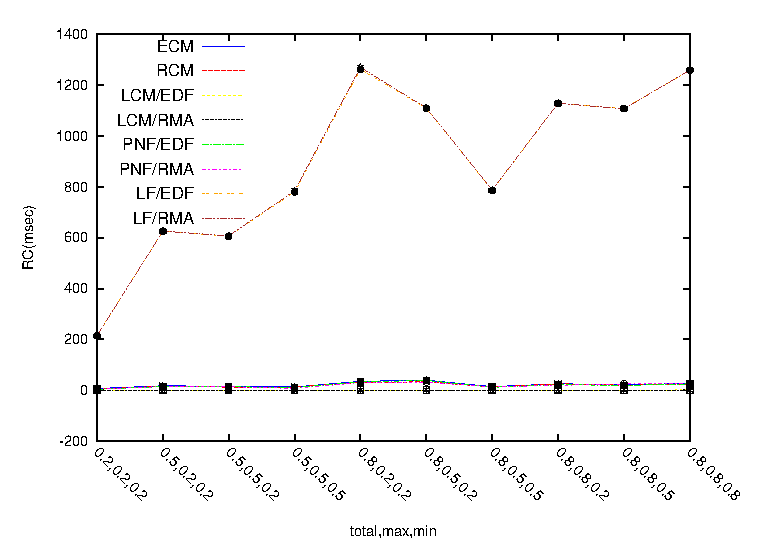
\includegraphics[scale=0.7]
{figures/Abr_dur_5t_1obj_1wr.eps}
\label{fig:pnf_results_1_obj_all}
}
~
\subfigure[ECM, RCM, LCM, PNF]{
\includegraphics[scale=0.7]
{figures/Abr_dur_5t_1obj_1wr_without_lf.eps}
\label{fig:pnf_results_1_obj_without_lock_free}
}
\caption{Average retry cost for 1 object per transaction for different values of total, maximum and minimum atomic section length under: a) all synchronization techniques. b) only contention managers. }
\label{fig:pnf_results_uniobject}
\end{figure}


\begin{figure}
\centering

\subfigure[Task set 1]{
\includegraphics[scale=0.7]
{figures/Abr_dur_4t_5obj_1wr.eps}
\label{fig-RC-pnf-4t}
}
~
\subfigure[Task set 2]{
\includegraphics[scale=0.7]
{figures/Abr_dur_8t_9obj_1wr.eps}
\label{fig-RC-pnf-8t}
}
~
\subfigure[Task set 3]{
\includegraphics[scale=0.7]{figures/Abr_dur_20t_21obj_1wr.eps}
\label{fig-RC-pnf-20t}
}

\caption{Average retry cost for different values of total, maximum and minimum atomic section length for: a) 4 tasks. b) 8 tasks. c) 20 tasks. }
\label{fig:pnf_results_multiobject}
\end{figure}

%%%%%%%%%%%%%%%%%%%%%%%%%%%%%%%%

\chapter{\label{conclusions}Conclusions, Contributions, and Proposed Post Preliminary-Exam Work
}
\markright{Mohammed Elshambakey \hfill Chapter 7. Conclusions, Contributions, and Future Work \hfill}

we consider STM for concurrency control in multicore real-time software. Doing so will require bounding transactional  retries, as real-time threads, which subsume transactions, must satisfy time constraints.  Retry bounds in STM are dependent on the CM policy at hand (analogous to the way thread response time bounds are scheduler-dependent). Thus, real-time CM is logical.

We investigate and design a number of real-time CMs. The first two CMs are directly based on dynamic and static priority of underlying tasks. Earliest Deadline-First CM with G-EDF scheduler (ECM) resolves conflicts based on absolute deadline of the underlying instances. Rate Monotonic Assignment with G-RMA scheduler (RCM) resolves conflicts based on period of underlying instances. We analyze retry cost and response time under ECM and RCM. We analytically and experimentally compare their schedulability against lock-free method.

ECM and RCM conserve the semantics of the underlying real-time scheduler. This conservative approach results in a maximum retry cost- for a single transaction due to another transaction- of double the maximum atomic section length among all tasks. So, another CM is developed to reduce this retry cost. Length-based CM (LCM) considers not only static/dynamic priority of underlying instance, but also length of the interfering transaction compared to remaining length of interfered transaction. LCM is used with G-EDF and G-RMA. Although it can reduce retry cost, but it suffers from priority inversion. By proper choice of different parameters, additional cost due to priority inversion can be kept lower than reduced retry cost. Thus, the net result will be lower response time for tasks using LCM with G-EDF/G-RMA. We analyze retry cost and response time of LCM. We analytically and experimentally compare LCM schedulability against ECM, RCM and lock-free.

ECM, RCM and LCM are affected by transitive retry. Transitive retry enforces a transaction to abort and retry due to another non-conflicting transaction. Transitive retry appears when multiple objects exist per transaction. So, we develop the Priority-based with Negative value and First access (PNF) contention manager. PNF avoids transitive retry and deals better with multiple objects than previous contention managers. PNF also tries to optimize processor usage by lowering priority of the job underlying retrying transaction. Thus, other jobs can proceed if there is no conflict. We upper bound retry cost and response time for PNF when used with G-EDF and G-RMA. Schedulability is compared between PNF on one side and ECM, RCM, LCM and lock-free on the other. We experimentally compare retry cost of PNF compared to other synchronization techniques.

\section{Contribution}

We design a number of contention managers that try to preserver real-time constraints besides data accuracy. Designing CMs is straightforward. The simplest logic is to keep the rational of the underlying real-time scheduler. This was shown in ECM and RCM. ECM allows transaction with earliest absolute deadline (dynamic priority) to commit first. RCM allows transaction with smallest period (fixed priority) to commit first. We derived upper bounds for retry cost and response time under both ECM and RCM. Lock-free schedulability was compared analytically and experimentally to schedulability of ECM and RCM. Under both ECM and RCM, a task incurs $2.s_{max}$ retry cost for each of its atomic sections due to a conflict with another task's atomic section. Retries under RCM and lock-free are affected by a larger number of conflicting task instances than under ECM. While task retries under ECM and lock-free are affected by all other tasks, retries under RCM are affected only by higher priority tasks. 

STM and lock-free have similar parameters that affect their retry costs---i.e., the number of conflicting jobs and how many times they access shared objects. The $s_{max}/r_{max}$ ratio determines whether STM is better or as good as lock-free. For ECM, this ratio cannot exceed 1, and it can be 1/2 for higher number of conflicting tasks. For RCM, for the common case, $s_{max}$ must be 1/2 of $r_{max}$, and in some cases, $s_{max}$ can be larger than $r_{max}$ by many orders of magnitude.

We present Length-based contention manager (LCM) that is used with G-EDF and G-RMA. LCM tries to compromise between priority of transactions (which is priority of the underlying task), and remaining execution time of interfered transaction. As the remaining execution time of the interfered transaction decreases, it will be useless to abort it while it can shortly commit. To abort the interfered transaction or not, is determined by a $\alpha$ and $\psi$. $\alpha$ ranges between 0 and 1. When $\alpha \rightarrow 0$, LCM acts in a first-in-first-out manner. When $\alpha\rightarrow1$, G-EDF/LCM acts like ECM, and G-RMA/LCM acts like RCM. We derived upper bounds on retry cost and response time under LCM. We also compared schedulability of LCM against ECM, RCM and lock-free. We identified the conditions under which LCM performs better than the other synchronization techniques. LCM reduces retry cost  of each atmic section to $(1+\alpha_{max})s_{max}$ instead of $2.s_{max}$ in case of ECM and RCM. In ECM and RCM, tasks do not retry due to lower priority tasks, whereas in LCM, they do so. In G-EDF/LCM, retry due to a lower priority job is encountered only from a task $\tau_{j}$'s last job instance during $\tau_{i}$'s period. This is not the case with G-RMA/LCM, because,  each higher priority task can be aborted and retried by any job instance of lower priority tasks. Schedulability of G-EDF/LCM and G-RMA/LCM is better or equal to ECM and RCM, respectively, by proper choices for $\alpha_{min}$ and $\alpha_{max}$. Schedulability of G-EDF/LCM is better than retry-loop lock-free synchronization for G-EDF if the upper bound on $s_{max}/r_{max}$ is between 0.5 and 2, which is higher than that achieved by ECM.

ECM, RCM and LCM suffer from transitive retry in case of multi-objects per transaction. So, we introduced Priority-based with Negative value and First access (PNF) contention manager. PNF avoids transitive retry effect suffered by ECM, RCM and LCM in case of multiple objects per transaction. PNF tries to optimize processor usage by lower priority of aborted transaction. This way, other tasks can proceed if they do no conflict with others. PNF implementation is not as simple as other CMs.
For previous contention managers, we upper bounded their retry cost and response times. We compared their schedulability to identify the conditions to prefer one of the them over the others. We also compared their schedulability against schedulability of lock-free method. We also compared retry cost of previous synchronization techniques.

\section{Post Preliminary-Exam Work}

We propose the following post preliminary exam work:
\begin{itemize}

\item \textbf{Analytical and experimental comparison between developed CMs and real-time locking protocols}
It has been said that lock-free and wait-free methods offer numerous advantages over locking protocols, but locking protocols are still of wide use in real-time systems due to simpler programming and analysis than lock-free. Thus, it is desired to compares different CMs against real-time locking protocols. Examples of real-time locking protocols include PCP and its variants~\cite{chen1990dynamic,6031129,Rajkumar:1991:SRS:532621,sha1990priority}, multiprocessor PCP (MPCP)~\cite{lakshmanan2009coordinated,rajkumar2002real,chen1998multiprocessor,easwaran2009resource}, SRP~\cite{lopez2004utilization}, multiprocessor SRP (MSRP)~\cite{gai2003comparison}, PIP~\cite{easwaran2009resource}, FMLP~\cite{key-4,brandenburg2008implementation,holman2006locking} and OMLP~\cite{Baruah:2007:TMG:1338441.1338647}. OMLP and FMLP are similar, and FMLP was found to be superior to other protocols~\cite{brandenburg2008comparison}.

\item \textbf{Contention manager development for nested transactions}
Transactions can be nested \textit{linearly}, where each transaction has at most one pending transaction~\cite{Moss2006186}. Nesting can also be done in \textit{parallel} where transactions execute concurrently within the same parent~\cite{volos2009nepaltm}. Linear nesting can be \textit{1) flat:} If a child transaction aborts, then parent also aborts. If a child commits, no effect is taken until the parent commits. Modifications made by child transaction is seen only be the parent . \textit{2) Closed:} Similar to \textit{flat nesting} except that if a child transaction aborts, parent does not have to abort. \textit{3) Open:} If a child transaction commits, its modifications is seen not only by the parent, but also by other non-surrounding transactions. If parent aborts after child commits, child modifications are still valid. It is required to extend the proposed real-time CMs (or develop new ones) to handle some or all types of transaction nesting.

\item \textbf{Combine both LCM and PNF} LCM is designed to reduce the retry cost of one transaction when it is interfered close to its end of execution. PNF is designed to avoid transitive retry in case of multiple objects per transactions. One goal is to combine benefits of both algorithms.

\item \textbf{Investigate other criterion for contention managers to further reduced retry cost} Criterion other than or combined with priority, transaction length and first access may be used to produce better contention managers.

\end{itemize}



% If you are using BibTeX, uncomment the following:
% \thebibliography
%
% Otherwise, uncomment the following:
% \chapter*{Bibliography}

%%%%%%%%%%%%%%%%%%%%%%%%%%%%%%%%
\bibliographystyle{plain}
\bibliography{global_bibliography}
%\bibliography{/e/lectures/real-time/PhD-work/STM/writing/global_bibliography}
\markright{Mohammed Elshambakey \hfill Bibliography \hfill}

% \appendix

% In LaTeX, each appendix is a "chapter"
% \chapter{Program Source}
%%%%%%%%%%%%%%%%%
%
% Include an EPS figure with this command:
%   \epsffile{filename.eps}
%

%%%%%%%%%%%%%%%%
%
% Do tables like this:
\begin{comment}
 \begin{table}
 \caption{The Graduate School wants captions above the tables.}
\begin{center}
 \begin{tabular}{ccc}
 x & 1 & 2 \\ \hline
 1 & 1 & 2 \\
 2 & 2 & 4 \\ \hline
 \end{tabular}
\end{center}
 \end{table}
\end{comment}

\end{document}